\section{Group -- Condenser Equipment}\label{group-condenser-equipment}

\subsection{Equipment Types}\label{equipment-types}

In each \hyperref[condenserequipmentlist]{CondenserEquipmentList}, various equipment types and names must be given. Each type-name pair must then have a corresponding equipment definition. This subsection lists the various equipment types that are available and examples from an IDF. Where appropriate, notes and comments on the input structure are provided.

\subsection{CoolingTower:SingleSpeed}\label{coolingtowersinglespeed}

Cooling towers are components that may be assigned to condenser loops. The cooling tower is modeled as a counterflow heat exchanger with a single-speed fan (induced draft configuration) based on Merkel's theory. The user must define tower performance via one of two methods: design heat transfer coefficient-area product (UA) and design water flow rate, or nominal tower capacity at a specific rating point. Regardless of which method is chosen, the design airflow rate and corresponding fan power must be specified. The model will also account for tower performance in the ``free convection'' regime, when the tower fan is off but the water pump remains on and heat transfer still occurs (albeit at a low level). If the user wants the model to account for ``free convection'', they must specify the corresponding airflow rate and heat transfer coefficient-area product (UA), or the nominal tower capacity during this mode of operation.

The cooling tower seeks to maintain the temperature of the water exiting the cooling tower at (or below) a set point. The set point schedule value is defined by the field ``Condenser Loop Temperature Setpoint Node Name or Reference'' for the \hyperref[condenserloop]{CondenserLoop} object. The model first checks to determine the impact of ``free convection'', if specified by the user, on the tower exiting water temperature. If the exiting water temperature based on ``free convection'' is at or below the set point, then the tower fan is not turned on. If the exiting water temperature based on ``free convection'' is below the set point, the tower will operate in FluidBypass mode -- portion of the water goes through the tower media and gets cooled while the remaining water flow gets bypassed, two water flows then mix together trying to meet the water setpoint temperature. If the exiting water temperature remains above the set point after ``free convection'' is modeled, then the tower fan is turned on to reduce the exiting water temperature to the set point. If the capacity control is FanCycling, the model assumes that part-load operation is represented by a simple linear interpolation between two steady-state regimes (i.e., tower fan on for the entire simulation timestep and tower fan off for the entire simulation timestep). Cyclic losses are not taken into account. If the capacity control is FluidBypass, the model determines the fraction of water flow to be bypassed while the remaining water goes through the tower cooling media and gets cooled, then the two water flows mix to meet the setpoint temperature. In this case, the fan runs at full speed for the entire timestep.

Cooling towers here are ``wet'' and consume water through evaporation, drift, and blowdown. The model can be used to predict water consumed by the towers. The last six input fields are optional and provide methods of controlling details of the water consumption calculations. The user can specify connections to the rest of the buildings water system by providing the name of a water storage tanks (i.e.~\hyperref[waterusestorage]{WaterUse:Storage} objects).

For the operation of multi-cell towers, the first step is to determine the number of cells to operate based on the cell control method -- between the minimum number of cells subject to the maximum water flow rate fraction per cell, and maximum number of cells subject to the minimum water flow rate fraction per cell. If the calculated cells do not meet the loads, additional cells will be operating to help meet the loads. Inside each cell, the existing capacity controls still apply.

For multi-cell towers, the following inputs are assumed to be for the entire tower including all cells:

\begin{itemize}
\item
  Design Water Flow Rate; Design Air Flow Rate; Fan Power at Design Air Flow Rate;
\item
  Air Flow Rate in Free Convection Regime; Nominal Capacity; Free Convection Capacity
\item
  BASIN HEATER (we assume that there is a common basin)
\end{itemize}

\subsubsection{Inputs}\label{inputs-007}

\paragraph{Field: Name}\label{field-name-006}

This alpha field contains the identifying name for the cooling tower.

\paragraph{Field: Water Inlet Node Name}\label{field-water-inlet-node-name}

This alpha field contains the identifying name for the cooling tower's water inlet node.

\paragraph{Field: Water Outlet Node Name}\label{field-water-outlet-node-name}

This alpha field contains the identifying name for the cooling tower's water outlet node.

\paragraph{Field: Design Water Flow Rate}\label{field-design-water-flow-rate}

This numeric field contains the design water flow rate through the tower in m\(^{3}\)/s. This value is the flow rate of the condenser loop water being cooled by the tower (not the flow rate of water being sprayed on the outside of the heat exchange coil). If the input field ``Performance Input Method'' is specified as ``UFactorTimesAreaAndDesignWaterFlowRate'', then a water flow rate greater than zero must be defined or the field can be autosized. If autosized, a Plant Sizing object must be defined and the design water flow rate is derived from the design load to be rejected by the condenser loop and the design loop delta T (Ref. Sizing and Input for Design Calculations and Component Autosizing sections). If ``Performance Input Method'' is specified as ``NominalCapacity'', then this field must be left blank since the model automatically assumes a water flow rate of 5.382E-8 m3/s per watt (3 gpm/ton) of tower capacity specified in the field ``Nominal Capacity''.

\paragraph{Field: Design Air Flow Rate}\label{field-design-air-flow-rate}

This numeric field contains the design air flow rate induced by the tower fan in m\(^{3}\)/s. A value greater than zero must be defined regardless of the tower performance input method. Alternately, this field can be autosized. If autosized, the design air flow rate is calculated as follows:

\begin{equation}
Design\;Air\;Flow\;Rate = \frac{{0.5{\rho_{air}}(Fan\;power\;at\;Design\;Air\;Flow\;Rate)}}{{190.}}
\end{equation}

where a fan pressure rise of 190 Pascals and total fan efficiency of 0.5 are assumed.

\paragraph{Field: Design Fan Power}

This numeric field contains the fan power (in watts) at the design air flow rate specified in the previous field. A value greater than zero must be specified regardless of the tower performance input method, or this field can be autosized. If autosized, the fan power is calculated as follows:

If``Performance Input Method'' is specified as ``\emph{UFactorTimesAreaAndDesignWaterFlowRate}'', then

\begin{equation}
Fan\;power = 0.0105\cdot {\rho_{water}}\cdot {C_{p,water}}\cdot Design\;Water\;Flow\;Rate\cdot Design\;Loop\Delta T
\end{equation}

is used.

If``Performance Input Method'' is specified as ``\emph{NominalCapacity}'', then

\begin{equation}
Fan\;power = 0.0105\cdot Tower\;Nominal\;Capacity
\end{equation}

is used.

\paragraph{Field: Design U-Factor Times Area Value}\label{field-design-u-factor-times-area-value}

This numeric field contains the heat transfer coefficient-area product (UA) in watts per Kelvin corresponding to the design air and water flow rates specified above. If the input field ``Performance Input Method'' is specified as ``UFactorTimesAreaAndDesignWaterFlowRate'', then a UA value greater than zero but less than or equal to 300,000 must be defined, or the field can be autosized. If autosized, a Plant Sizing object must be defined and the design tower UA value is derived from the design load to be rejected by the condenser loop and the design loop delta T (Ref. Sizing and Input for Design Calculations and Component Autosizing sections), assuming a tower water inlet temperature of 35C and tower inlet air at 35C drybulb/25.6C wetbulb. If ``Performance Input Method'' is specified as ``NominalCapacity'', then this field must be left blank since the model automatically calculates the tower UA based on the tower capacity specified in the field ``Nominal Capacity''.

\paragraph{Field: Free Convection Regime Air Flow Rate}\label{fieldfree-convection-regime-air-flow-rate}

This numeric field contains the air flow rate (m\(^{3}\)/s) when the tower is in the ``free convection'' regime (water flow exists but tower fan is turned off). This value must be less than the value specified for the field ``Design Air Flow Rate''. This field may be autocalculated, in which case it is set to a fraction of the ``Design Air Flow Rate'' determined in the following input field. If the user does not wish to model ``free convection'' and is using the Performance Input Method ``UFactorTimesAreaAndDesignWaterFlowRate'', then this field should be set to 0.0. If the user specifies the U-Factor Times Area Value at Free Convection Air Flow Rate or Free Convection Capacity as a value greater than zero, then the free convection air flow rate must be specified greater than 0.0.

\paragraph{Field: Free Convection Regime Air Flow Rate Sizing Factor}\label{field-free-convection-regime-air-flow-rate-sizing-factor}

This numeric field contains the sizing factor to use when calculating the free convection regime air flow rate.~ The default is 0.1.

\paragraph{Field: Free Convection Regime U-Factor Times Area Value}\label{fieldfree-convection-regime-u-factor-times-area-value}

This numeric field contains the heat transfer coefficient-area product (W/K) when the tower is in the ``free convection'' regime (water flow exists but tower fan is turned off). This value must be less than the value specified for the field ``U-Factor Times Area Value at Design Air Flow Rate''. This field may be autosized, in which case it is set to a fraction of the ``U-Factor Times Area Value at Design Air Flow Rate'' determined in the following input field. If the user does not wish to model ``free convection'' and is using the~ Performance Input Method ``UFactorTimesAreaAndDesignWaterFlowRate'', then this field should be set to 0.0. If ``Performance Input Method'' is specified as ``NominalCapacity'', then this field must be left blank since the model automatically calculates the tower UA based on the tower capacity specified in the field ``Free Convection Capacity''.\textbackslash{}

\paragraph{Field: Free Convection U-Factor Times Area Value Sizing Factor}\label{field-free-convection-u-factor-times-area-value-sizing-factor}

This numeric field contains the sizing factor to use when calculating the free convection regime U-Factor times area value.~ The default is 0.1.

\paragraph{Field: Performance Input Method}\label{field-performance-input-method}

This alpha field contains the method by which the user will specify tower performance: ``\textbf{UFactorTimesAreaAndDesignWaterFlowRate}'' or ``\textbf{NominalCapacity}''. If this field is left blank in the input data file, the default input method is assumed to be ``\textbf{UFactorTimesAreaAndDesignWaterFlowRate}''. If the method ``\textbf{UFactorTimesAreaAndDesignWaterFlowRate}'' is selected, then the user must enter design UA values, design water flow rates and air flow rates as described for the previous input fields. If the method ``NominalCapacity'' is selected then the fields ``Design Water Flow Rate'', ``U-Factor Times Area Value at Design Air Flow Rate'' and ``U-Factor Times Area Value at Free Convection Air Flow Rate'' must be left blank, but the fields ``Nominal Capacity'' and ``Free Convection Capacity'' must be entered as described below.

\paragraph{Field: Heat Rejection Capacity and Nominal Capacity Sizing Ratio}\label{field-heat-rejection-capacity-and-nominal-capacity-sizing-ratio}

This numeric field contains the value for the ratio of actual tower heat rejection to nominal capacity.~ This ratio is defined at entering water at 35C (95F), leaving water at 29.4C (85F), entering air at 25.6C (78F) wetbulb and 35C (95F) drybulb temperatures. Historically this ratio has been set at 1.25 based on the assumption that the tower must dissipate 0.25 W of compressor power for every what of heat removed at the chiller evaporator.~ The default is 1.25.

\paragraph{Field: Nominal Capacity}\label{field-nominal-capacity}

This numeric input field contains the ``nominal'' heat rejection capacity of the cooling tower in watts, with entering water at 35C (95F), leaving water at 29.4C (85F), entering air at 25.6C (78F) wetbulb and 35C (95F) drybulb temperatures. The design water flow rate is assumed to be 5.382E-8 m\(^{3}\)/s per watt of nominal capacity (3 gpm/ton). The value in the previous field times this nominal tower capacity gives the actual tower heat rejection at these operating conditions (based on historical assumption that the tower must dissipate additional heat from the compressor heat for heat removed at the evaporator).

\paragraph{Field: Free Convection Capacity}\label{field-free-convection-capacity}

This numeric input field contains the ``nominal'' heat rejection capacity of the cooling tower in watts when the tower is in the ``free convection'' regime (water flow exists but tower fan is turned off), with entering water at 35C (95F), leaving water at 29.4C (85F), entering air at 25.6C (78F) wetbulb and 35C (95F) drybulb temperatures. The design water flow rate is assumed to be 5.382E-8 m\(^{3}\)/s per watt of nominal tower capacity (input field above). The heat rejection capacity and nominal capacity sizing ratio is applied to this free convection tower capacity to give the actual tower heat rejection at these operating conditions (typical value is 1.25 based on historical assumption that the tower must dissipate 0.25W of compressor heat for every watt of heat removed by the evaporator). The value specified for this field must be less than the value specified for the field ``Tower Nominal Capacity''. If the user does not wish to model ``free convection'', then this field should be set to 0.0. If the user specifies a value greater than zero, then the ``Air Flow Rate in Free Convection Regime'' field must contain a value greater than zero. This field can be automatically calculated using the sizing factor in the following field.

\paragraph{Field: Free Convection Nominal Capacity Sizing Factor}\label{field-free-convection-nominal-capacity-sizing-factor}

This numeric field contains the sizing factor to use when calculating the Free Convection Capacity. The default is 0.1.

\paragraph{Field: Design Inlet Air Dry-Bulb Temperature}\label{field-design-inlet-air-drybulb-temperature}

This numeric field specifies the design inlet air dry-bulb temperature of the tower. The default is \SI{35.0}{\celsius}.

\paragraph{Field: Design Inlet Air Wet-Bulb Temperature}\label{field-design-inlet-air-wetbulb-temperature}

This numeric field specifies the design inlet air wet-bulb temperature of the tower. The default is \SI{25.6}{\celsius}.

\paragraph{Field: Design Approach Temperature}

This numeric field specifies the design approach temperature of the tower corresponding to the design inlet air wet-bulb temperature and the design temperature range.
The approach temperature should be the outlet water temperature minus the inlet air wet-bulb temperature at design conditions.
This parameter is autosizable and when autosized it is set to \SI{3.9}{\celsius}.

\paragraph{Field: Design Temperature Range}\label{field-design-temperature-range}

This numeric field specifies the design temperature range of the tower corresponding to the design inlet air wet-bulb temperature and the design approach temperature.
The design range  should be the inlet water temperature minus the outlet water temperature at design conditions.
This parameter is autosizable and when autosized it is set to \SI{5.5}{\celsius}.

\paragraph{Field: Basin Heater Capacity}\label{field-basin-heater-capacity}

This numeric field contains the capacity of the tower's electric basin heater in watts per degree Kelvin. This field is used in conjunction with the Basin Heater Setpoint Temperature described in the following field. The basin heater electric power is equal to this field multiplied by the difference between the basin heater set point temperature and the outdoor dry-bulb temperature. The basin heater only operates when the tower fan is off and water is not flowing through the tower, regardless of the basin heater schedule described below. The basin heater capacity must be greater than or equal to zero, with a default value of zero if this field is left blank.

\paragraph{Field: Basin Heater Setpoint Temperature}\label{field-basin-heater-setpoint-temperature}

This numeric field contains the set point temperature (°C) for the basin heater described in the previous field. The basin heater is active when the outdoor air dry-bulb temperature falls below this setpoint temperature, as long as the tower fan is off and water is not flowing through the tower. This set point temperature must be greater than or equal to 2˚C, and the default value is 2˚C if this field is left blank.

\paragraph{Field: Basin Heater Operating Schedule Name}\label{field-basin-heater-operating-schedule-name}

This alpha field contains the name of the basin heater operating schedule. The basin heater operating schedule is assumed to be an on/off schedule and the heater is available to operate any time the schedule value is greater than 0. The basin heater operates when scheduled on and the outdoor air dry-bulb temperature is below the set point temperature described in the previous field. If this field is left blank, the basin heater is available to operate throughout the simulation. Regardless of this schedule, the basin heater may only operate when the cooling tower fan is off and water is not flowing through the tower.

\paragraph{Field: Evaporation Loss Mode}\label{field-evaporation-loss-mode}

This field is used to choose which method is used to model the amount of water evaporated by the cooling tower. There are two options: \textbf{LossFactor} or \textbf{SaturatedExit}. The default is SaturatedExit. The user-defined loss factor is entered in the following field. By assuming that the air leaving the tower is saturated, the evaporation can be directly calculated using moist air engineering calculations with data available within the cooling tower model (and does not require additional user input).

\paragraph{Field: Evaporation Loss Factor}\label{field-evaporation-loss-factor}

This field is used to specify the rate of water evaporated from the cooling tower and lost to the outside air {[}percent/K{]}. This field is only used if the Evaporation Calculation Mode is set to \textbf{LossFactor}. The evaporation loss is then calculated as a fraction of the circulating condenser water flow and varies with the temperature change in the condenser water. The value entered here is in units of percent-per-degree Kelvin. The evaporation rate will equal this value times each degree Kelvin of temperature drop in the condenser water. Typical values are from 0.15 to 0.27 {[}percent/K{]}. The default is 0.2.

\paragraph{Field: Drift Loss Percent}\label{field-drift-loss-percent}

This field is used to specify the rate of water lost to the exiting air as entrained droplets {[}\%{]}. The drift loss is a percent of the condenser water flow. Typical values for towers with efficient drift eliminators are between 0.002 and 0.2\% of the condenser water flow rate. The default value is 0.008\%.

\paragraph{Field: Blowdown Calculation Mode}\label{field-blowdown-calculation-mode}

This field specifies which method is used to determine blowdown rates. There two options \textbf{ConcentrationRatio} or \textbf{ScheduledRate}. The choice will determine which of the two models below is used. The default is ConcentrationRatio.

\paragraph{Field: Blowdown Concentration Ratio}\label{field-blowdown-concentration-ratio}

This field is used to dynamically adjust the rate of blowdown in the cooling tower as a function of the rate of evaporation. Blowdown is water intentionally drained from the tower in order to offset the build up of solids in the water that would otherwise occur because of evaporation. The value entered here is dimensionless. It can be characterized as the ratio of solids in the blowdown water to solids in the make up water. Typical values for tower operation are 3 to 5. The default value is 3.

\paragraph{Field: Blowdown Makeup Water Usage Schedule Name}\label{field-blowdown-makeup-water-usage-schedule-name}

This alpha field contains the name of the schedule used to define the amount of water (m\(^{3}\)/s) flushed from the basin on a periodic basis to purge the tower of mineral scale build-up and other contaminants. This schedule is only used if the Blowdown Calculation Mode is set to ScheduledRate. The amount of water use due to blowdown depends on the makeup water quality and is specific to each geographical location. Typical values range from 0.0002 to 0.0013 m\(^{3}\)/s (17.3 to 112.3 m\(^{3}\)/day). This water usage is in addition to the amount of water lost to the atmosphere due to evaporation and/or drift. Since blowdown occurs when the basin water contaminant concentration is high, blowdown only occurs when the cooling tower is active and water is flowing through the tower (regardless of the water usage defined by this schedule).

\paragraph{Field: Supply Water Storage Tank Name}\label{field-supply-water-storage-tank-name}

This field is optional. It is used to describe where the tower obtains water used for evaporative cooling. If blank or omitted, then the tower will obtain water directly from the mains. If the name of a \hyperref[waterusestorage]{WaterUse:Storage} object is used here, then the tower will obtain its water from that tank. If a tank is specified, the tower will attempt to obtain all the water it uses from the tank. However if the tank cannot provide all the water the tower needs, then the tower will still operate and obtain the rest of the water it needs from the mains (referred to as `Starved' water).

\paragraph{Field: Outdoor Air Inlet Node Name}\label{field-outdoor-air-inlet-node-name-000}

This optional alpha field specifies the outdoor air node name used to define the conditions of the air entering the cooling tower. If this field is left blank, the outdoor air conditions entering the cooling tower are taken directly from the weather data. If this field is not blank, the node name specified must also be specified in an \hyperref[outdoorairnode]{OutdoorAir:Node} object where the height of the node is taken into consideration when calculating outdoor air conditions from the weather data. Alternately, the node name may be specified in an \hyperref[outdoorairnodelist]{OutdoorAir:NodeList} object where the outdoor air conditions are taken directly from the weather data.

\paragraph{Field:Capacity Control}\label{fieldcapacity-control}

This alpha field contains the cooling capacity control for the cooling tower. Two choices are available: \textbf{FanCycling} and \textbf{FluidBypass}. During part-load conditions, there are two ways to maintain the exiting water temperature at the setpoint: either cycling the tower fan, or bypassing portion of the tower water with a three-way valve. For FluidBypass, the tower fan still runs at full speed for the entire timestep, but only portion of the water flow goes through the cooling tower media to get cooled while the remaining portion of the water flow gets bypassed. Two water flows then mix at the common water sump to meet the setpoint temperature.

\paragraph{Field: Number of Cells}\label{field-number-of-cells}

This integer field contains the number of cells in the multi-cell cooling tower. If not entered, the program will assume it is a single-cell cooling tower

\paragraph{Field: Cell Control}\label{field-cell-control}

This alpha field specifies the method used to control the number of cells used to meet the load, the two choices are:

\textbf{MinimalCell} : the program will use minimal number of cells needed, all other cells will be shut down with no water flow. It will attempt to use as few cells as possible to cool the fluid. In no case, however, will the flow per cell be allowed to exceed its maximum value defined by the \emph{Maximum Water Flow Rate Fraction.}

\textbf{MaximalCell}: As many cells as possible will be turned on. In no case, however, will the flow per cell be allowed to drop below its minimum value specified by the \emph{Minimum Water Flow Rate Fraction}.

If this field is left blank, the default value is \textit{MaximalCell}.

\paragraph{Field: Cell Minimum Water Flow Rate Fraction}\label{field-cell-minimum-water-flow-rate-fraction}

This numeric field specifies the allowable smallest fraction of the design water flow rate. Flows less than this value will commonly result in fluid distribution problems; the pressure at each nozzle will be too weak for the fluid to be sprayed out in the correct pattern, not all the fill would be wet. If this field is left blank, the default value is 0.33.

\paragraph{Field: Cell Maximum~ Water Flow Rate Fraction}\label{field-cell-maximum-water-flow-rate-fraction}

This numeric field specifies the allowable largest fraction of the design water flow rate. If this field is left blank, the default value is 2.5.

\paragraph{Field: Sizing Factor}\label{sizing-factor-01}

This optional numeric field allows the user to specify a sizing factor for this component. The sizing factor is used when the component design inputs are autosized: the autosizing calculations are performed as usual and the results are multiplied by the sizing factor. Sizing factor allows the user to size a component to meet part of the design load while continuing to use the autosizing feature. For this component the inputs that would be altered by the sizing factor are:

1.~~~~Design Water Flow Rate;

2.~~~~Design Air Flow Rate;

3.~~~~Fan Power at Design Air Flow Rate;

4.~~~~U-Factor Times Area Value at Design Air Flow Rate;

5.~~~~Air Flow Rate in Free Convection Regime;

6.~~~~U-Factor Times Area Value at Free Convection Air Flow Rate.

Note that the U-Factor Times Area Value at Design Air Flow Rate is not \emph{multiplied} by the Sizing Factor. Instead the design tower load is multiplied by the sizing factor and the design UA then calculated as usual. The U-Factor Times Area Value at Free Convection Air Flow Rate is set to 10\% of the new design Tower UA.

\paragraph{Field: End-Use Subcategory}\label{end-use-subcategory-01}

This optional field allows you to specify a user-defined end-use subcategory, e.g., ``Process''. A new meter for reporting is created for each unique subcategory (ref: \hyperref[outputmeter-and-outputmetermeterfileonly]{Output:Meter} objects). Any text may be used here to further subcategorize the end-uses in the ABUPS End Uses by Subcategory table and in the LEED Summary EAp2-4/5 Performance Rating Method Compliance table. If this field is omitted or blank, the cooling tower will be assigned to the ``General'' end-use subcategory.


Three examples of an IDF specification for this object are shown below:

\begin{lstlisting}

  CoolingTower:SingleSpeed,
    My Tower,                     !- Name
    Condenser Tower Inlet Node,   !- Water Inlet Node Name
    Condenser Tower Outlet Node,  !- Water Outlet Node Name
    .0011,                        !- Design Water Flow Rate {m3/s}
    16.0,                         !- Design Air Flow Rate {m3/s}
    10000.,                       !- Design Fan Power {W}
    3500.,                        !- Design U-Factor Times Area Value {W/K}
    0.0,                          !- Free Convection Air Flow Rate {m3/s}
    ,                             !- Free Convection Air Flow Rate Sizing Factor
    0.0,                          !- Free Convection U-Factor Times Area Value {W/K}
    ,                             !- Free Convection U-Factor Times Area Value Sizing Factor
    UFactorTimesAreaAndDesignWaterFlowRate,   !- Performance Input Method
    ,                             !- Heat Rejection Capacity and Nominal Capacity Sizing Ratio
    ,                             !- Nominal Capacity {W}
    ,                             !- Free Convection Capacity {W}
    ,                             !- Free Convection Nominal Capacity Sizing Factor
    ,                             !- Design Inlet Air Dry-Bulb Temperature {C}
    ,                             !- Design Inlet Air Wet-Bulb Temperature {C}
    ,                             !- Design Approach Temperature {deltaC}
    ,                             !- Design Range Temperature {deltaC}
    ,                             !- Basin Heater Capacity {W/K}
    ,                             !- Basin Heater Setpoint Temperature {C}
    ,                             !- Basin Heater Operating Schedule Name
    ,                             !- Evaporation Loss Mode
    ,                             !- Evaporation Loss Factor {percent/K}
    ,                             !- Drift Loss Percent {percent}
    ,                             !- Blowdown Calculation Mode
    ,                             !- Blowdown Concentration Ratio
    ,                             !- Blowdown Makeup Water Usage Schedule Name
    ,                             !- Supply Water Storage Tank Name
    ,                             !- Outdoor Air Inlet Node Name
    FluidBypass,                  !- Capacity Control
    4,                            !- Number of Cells
    MinimalCell,                  !- Cell Control
    ,                             !- Cell Minimum  Water Flow Rate Fraction
    ,                             !- Cell Maximum Water Flow Rate Fraction
    1.0000;                       !- Sizing Factor

  CoolingTower:SingleSpeed,
    My Tower,                   !- Name
    Condenser Tower Inlet Node, !- Water Inlet Node Name
    Condenser Tower Outlet Node,!- Water Outlet Node Name
    ,                           !- Design Water Flow Rate {m3/s}
    Autosize,                   !- Design Air Flow Rate {m3/s}
    1000.,                      !- Design Fan Power {W}
    ,                           !- Design U-Factor Times Area Value {W/K}
    autocalculate,              !- Free Convection Air Flow Rate {m3/s}
    ,                           !- Free Convection Air Flow Rate Sizing Factor
    autocalculate,              !- Free Convection U-Factor Times Area Value {W/K}
    ,                           !- Free Convection U-Factor Times Area Value Sizing Factor
    NominalCapacity,            !- Performance Input Method
    ,                           !- Heat Rejection Capacity and Nominal Capacity Sizing Ratio
    95250.,                     !- Nominal Capacity {W}
    9525.;                      !- Free Convection Capacity {W}

  CoolingTower:SingleSpeed,
    TowerWaterSys CoolTower, !- Name
    TowerWaterSys Pump-TowerWaterSys CoolTowerNode,  !- Water Inlet Node Name
    TowerWaterSys Supply Equipment Outlet Node,  !- Water Outlet Node Name
    AUTOSIZE,                !- Design Water Flow Rate {m3/s}
    AUTOSIZE,                !- Design Air Flow Rate {m3/s}
    AUTOSIZE,                !- Design Fan Power {W}
    AUTOSIZE,                !- Design U-Factor Times Area Value {W/K}
    autocalculate,           !- Free Convection Air Flow Rate {m3/s}
    ,                        !- Free Convection Air Flow Rate Sizing Factor
    autocalculate,           !- Free Convection U-Factor Times Area Value {W/K}
    ,                        !- Free Convection U-Factor Times Area Value Sizing Factor
    UFactorTimesAreaAndDesignWaterFlowRate,  !- Performance Input Method
    ,                        !- Heat Rejection Capacity and Nominal Capacity Sizing Ratio
    ,                        !- Nominal Capacity {W}
    ,                        !- Free Convection Capacity {W}
    ,                        !- Free Convection Nominal Capacity Sizing Factor
    ,                        !- Design Inlet Air Dry-Bulb Temperature {C}
    ,                        !- Design Inlet Air Wet-Bulb Temperature {C}
    ,                        !- Design Approach Temperature {deltaC}
    ,                        !- Design Range Temperature {deltaC}
    ,                        !- Basin Heater Capacity {W/K}
    ,                        !- Basin Heater Setpoint Temperature {C}
    ,                        !- Basin Heater Operating Schedule Name
    SaturatedExit,           !- Evaporation Loss Mode
    ,                        !- Evaporation Loss Factor {percent/K}
    0.0080,                  !- Drift Loss Percent {percent}
    ConcentrationRatio,      !- Blowdown Calculation Mode
    3.0000,                  !- Blowdown Concentration Ratio
    ,                        !- Blowdown Makeup Water Usage Schedule Name
    ,                        !- Supply Water Storage Tank Name
    TowerWaterSys CoolTower OA ref Node,  !- Outdoor Air Inlet Node Name
    FanCycling,              !- Capacity Control
    4,                       !- Number of Cells
    MinimalCell,             !- Cell Control
    ,                        !- Cell Minimum  Water Flow Rate Fraction
    ,                        !- Cell Maximum Water Flow Rate Fraction
    1.0000;                  !- Sizing Factor

  OutdoorAir:Node,
    TowerWaterSys CoolTower OA ref Node;  !- Name

\end{lstlisting}

\subsubsection{Outputs}\label{outputs-004}

\begin{itemize}
\item
  HVAC,Average,Cooling Tower Fan Electricity Rate {[}W{]}
\item
  HVAC,Sum,Cooling Tower Fan Electricity Energy {[}J{]}
\item
  HVAC,Average,Cooling Tower Heat Transfer Rate {[}W{]}
\item
  HVAC,Average,Cooling Tower Inlet Temperature {[}C{]}
\item
  HVAC,Average,Cooling Tower Outlet Temperature {[}C{]}
\item
  HVAC,Average,Cooling Tower Mass Flow Rate {[}kg/s{]}
\item
  HVAC,Average,Cooling Tower Bypass Fraction {[]}
\item
  HVAC,Average,Cooling Tower Fan Cycling Ratio {[]}
\item
  HVAC,Average,Cooling Tower Operating Cells Count {[]}
\end{itemize}

A tower uses either mains water or storage tank for make-up water.

\emph{When mains water is used:}

\begin{itemize}
\item
  HVAC,Average,Cooling Tower Make Up Water Volume Flow Rate~ {[}m3/s{]}
\item
  HVAC,Sum,Cooling Tower Make Up Water Volume {[}m3{]}
\item
  HVAC,Sum,Cooling Tower Make Up Mains Water Volume {[}m3{]}
\end{itemize}

\emph{When storage tank water is used:}

\begin{itemize}
\item
  HVAC,Average,Cooling Tower Make Up Water Volume Flow Rate~ {[}m3/s{]}
\item
  HVAC,Sum,Cooling Tower Make Up Water Volume {[}m3{]}
\item
  HVAC,Sum,Cooling Tower Storage Tank Water Volume Flow Rate {[}m3/s{]}
\item
  HVAC,Sum,Cooling Tower Storage Tank Water Volume {[}m3{]}
\item
  HVAC,Sum,Cooling Tower Starved Storage Tank Water Volume Flow Rate {[}m3/s{]}
\item
  HVAC,Sum,Cooling Tower Starved Storage Tank Water Volume {[}m3{]}
\item
  HVAC,Sum,Cooling Tower Make Up Mains Water Volume {[}m3{]}
\item
  HVAC,Average,Cooling Tower Water Evaporation Volume Flow Rate {[}m3/s{]}
\item
  HVAC,Sum,Cooling Tower Water Evaporation Volume {[}m3{]}
\item
  HVAC,Average,Cooling Tower Water Drift Volume Flow Rate {[}m3/s{]}
\item
  HVAC,Sum,Cooling Tower Water Drift Volume {[}m3{]}
\item
  HVAC,Average,Cooling Tower Water Blowdown Volume Flow Rate {[}m3/s{]}
\item
  HVAC,Sum,Cooling Tower Water Blowdown Volume {[}m3{]}
\end{itemize}

IF specified:

\begin{itemize}
\item
  HVAC,Average,Cooling Tower Basin Heater Electricity Rate {[}W{]}
\item
  HVAC,Sum,Cooling Tower Basin Heater Electricity Energy {[}J{]}
\end{itemize}

\paragraph{Cooling Tower Fan Electricity Rate {[}W{]}}\label{cooling-tower-fan-electric-power-w}

\paragraph{Cooling Tower Fan Electricity Energy {[}J{]}}\label{cooling-tower-fan-electric-energy-j}

These outputs are the electric power input to the tower fans. Consumption is metered on HeatRejection:Electricity, Electricity:Plant, and Electricity:Facility.

\paragraph{Cooling Tower Heat Transfer Rate {[}W{]}}\label{cooling-tower-heat-transfer-rate-w}

This is the rate at which heat is removed from the condenser water loop by the tower.

\paragraph{Cooling Tower Inlet Temperature {[}C{]}}\label{cooling-tower-inlet-temperature-c}

\paragraph{Cooling Tower Outlet Temperature {[}C{]}}\label{cooling-tower-outlet-temperature-c}

\paragraph{Cooling Tower Mass Flow Rate {[}kg/s{]}}\label{cooling-tower-mass-flow-rate-kgs}

These outputs are the tower water inlet and outlet temperatures, and mass flow rate of the circulating condenser water loop.

\paragraph{Cooling Tower Basin Heater Electricity Rate {[}W{]}}\label{cooling-tower-basin-heater-electric-power-w}

\paragraph{Cooling Tower Basin Heater Electricity Energy {[}J{]}}\label{cooling-tower-basin-heater-electric-energy-j}

These outputs are the electric power input to the tower basin heater. Consumption is metered on HeatRejection:Electricity, Electricity:Plant, and Electricity:Facility

\paragraph{Cooling Tower Make Up Water Volume Flow Rate {[}m3/s{]}}\label{cooling-tower-make-up-water-volume-flow-rate-m3s}

\paragraph{Cooling Tower Make Up Water Volume {[}m3{]}}\label{cooling-tower-make-up-water-volume-m3}

These outputs are the water consumed by the wet cooling tower for external water sprays used to augment heat transfer. This is the total of evaporation, drift, and blowdown.

\paragraph{Cooling Tower Water Evaporation Volume Flow Rate {[}m3/s{]}}\label{cooling-tower-water-evaporation-volume-flow-rate-m3s}

\paragraph{Cooling Tower Water Evaporation Volume {[}m3{]}}\label{cooling-tower-water-evaporation-volume-m3}

\paragraph{Cooling Tower Water Drift Volume Flow Rate {[}m3/s{]}}\label{cooling-tower-water-drift-volume-flow-rate-m3s}

\paragraph{Cooling Tower Water Drift Volume {[}m3{]}}\label{cooling-tower-water-drift-volume-m3}

\paragraph{Cooling Tower Water Blowdown Volume Flow Rate {[}m3/s{]}}\label{cooling-tower-water-blowdown-volume-flow-rate-m3s}

\paragraph{Cooling Tower Water Blowdown Volume {[}m3{]}}\label{cooling-tower-water-blowdown-volume-m3}

These outputs provide the breakdown of the different components of water use during cooling tower operation.

\paragraph{Cooling Tower Make Up Mains Water Volume {[}m3{]}}\label{cooling-tower-make-up-mains-water-volume-m3}

This is the volume of water drawn from mains service to feed the cooling tower.

If a water storage tank is used to provide water to the tower, then the following output variables will also be available.

\paragraph{Cooling Tower Storage Tank Water Volume Flow Rate {[}m3/s{]}}\label{cooling-tower-storage-tank-water-volume-flow-rate-m3s}

\paragraph{Cooling Tower Storage Tank Water Volume {[}m3{]}}\label{cooling-tower-storage-tank-water-volume-m3}

These are the rate and volume of water provided by the Water Storage Tank.

\paragraph{Cooling Tower Starved Storage Tank Water Volume Flow Rate {[}m3/s{]}}\label{cooling-tower-starved-storage-tank-water-volume-flow-rate-m3s}

\paragraph{Cooling Tower Starved Storage Tank Water Volume {[}m3{]}}\label{cooling-tower-starved-storage-tank-water-volume-m3}

These are the rate and volume of water the Storage Tank connections was not able to provide. The starved water is assumed to come from the mains. The tower's operation is not affected by a lack of storage tank water.

\paragraph{Cooling Tower Fan Cycling Ratio {[]}}\label{cooling-tower-fan-cycling-ratio}

This represents the fraction of a time-step when tower fan is on.

\paragraph{Cooling Tower Bypass Fraction {[]}}\label{cooling-tower-bypass-fraction}

This represents the fraction of a fluid bypassing the tower when a mixture of the tower fluid and tower return water is able to meet the set point temperature.

\paragraph{Cooling Tower Operating Cells Count {[]}}\label{cooling-tower-operating-cells-count}

This represents the number of cells operating at each time step.

\subsection{CoolingTower:TwoSpeed}\label{coolingtowertwospeed}

The two-speed cooling tower is modeled in a similar fashion to the single-speed tower. The cooling tower is modeled as a counterflow heat exchanger with a two-speed fan (induced draft configuration) based on Merkel's theory. The user must define tower performance via one of two methods: heat transfer coefficient-area product (UA) and design water flow rate, or nominal tower capacity at a specific rating point. Regardless of which method is chosen, the airflow rate and corresponding fan power at both high and low fan speed must be specified. The model will also account for tower performance in the ``free convection'' regime, when the tower fan is off but the water pump remains on and heat transfer still occurs (albeit at a low level). If the user wants the model to account for ``free convection'', they must specify the corresponding air flow rate and heat transfer coefficient-area product (UA), or the nominal tower capacity during this mode of operation.

The cooling tower seeks to maintain the temperature of the water exiting the cooling tower at (or below) a set point. The set point schedule value is defined by the field ``Condenser Loop Temperature Setpoint Node Name or Reference'' for the \hyperref[condenserloop]{CondenserLoop} object. The model first checks to determine the impact of ``free convection'', if specified by the user, on the tower exiting water temperature. If the exiting water temperature based on ``free convection'' is at or below the set point, then the tower fan is not turned on. If the exiting water temperature remains above the set point after ``free convection'' is modeled, then the tower fan is turned on at low speed to reduce the exiting water temperature. If operating the tower fan at low speed does not reduce the exiting water temperature to the set point, then the tower fan is increased to its high speed.

The model assumes that part-load operation is represented by a simple linear interpolation between two steady-state regimes (i.e., tower fan at high speed for the entire simulation timestep and tower fan at low speed for the entire simulation timestep, or tower fan at low speed for the entire simulation timestep and tower fan off for the entire simulation timestep). Cyclic losses are not taken into account.

Cooling towers here are ``wet'' and consume water through evaporation, drift, and blowdown. The model can be used to predict water consumed by the towers. The last six input fields are optional and provide methods of controlling details of the water consumption calculations. The user can specify connections to the rest of the buildings water system by providing the name of a \hyperref[waterusestorage]{WaterUse:Storage} object.

For the operation of multi-cell towers, the first step is to determine the number of cells to operate based on the cell control method -- between the minimum number of cells subject to the maximum water flow rate fraction per cell, and maximum number of cells subject to the minimum water flow rate fraction per cell. If the calculated cells do not meet the loads, additional cells will be operating to help meet the loads. Inside each cell, the existing capacity controls still apply.

For multi-cell towers, the following inputs are assumed to be for the entire tower including all cells:

\begin{itemize}
\item
  Design Water Flow Rate; Design Air Flow Rate; Fan Power at Design Air Flow Rate;
\item
  Air Flow Rate in Free Convection Regime; Nominal Capacity; Free Convection Capacity
\item
  BASIN HEATER (we assume that there is a common basin)
\end{itemize}

\subsubsection{Inputs}\label{inputs-1-006}

\paragraph{Field: Name}\label{ct-twospeed-field-name}

This alpha field contains the identifying name for the cooling tower.

\paragraph{Field: Water Inlet Node Name}\label{field-water-inlet-node-name-1}

This alpha field contains the identifying name for the cooling tower's water inlet node.

\paragraph{Field: Water Outlet Node Name}\label{field-water-outlet-node-name-1}

This alpha field contains the identifying name for the cooling tower's water outlet node.

\paragraph{Field: Design Water Flow Rate}\label{field-design-water-flow-rate-1}

This numeric field contains the design water flow rate through the tower in m\(^{3}\)/s. This value is the flow rate of the condenser loop water being cooled by the tower (not the flow rate of water being sprayed on the outside of the heat exchange coil). If the input field ``Performance Input Method'' is specified as ``UFactorTimesAreaAndDesignWaterFlowRate'', then a water flow rate greater than zero must be defined or the field can be autosized. If autosized, a Plant Sizing object must be defined and the design water flow rate is derived from the design load to be rejected by the condenser loop and the design loop delta T (Ref. Sizing and Input for Design Calculations and Component Autosizing sections). If ``Performance Input Method'' is specified as ``NominalCapacity'', then this field must be left blank since the model automatically assumes a design water flow rate of 5.382E-8 m3/s per watt (3 gpm/ton) of tower capacity specified in the field ``Tower High-Speed Nominal Capacity''.

\paragraph{Field: High Fan Speed Air Flow Rate}\label{field-high-fan-speed-air-flow-rate}

This numeric field contains the tower air flow rate at high fan speed in m\(^{3}\)/s. A value greater than zero must be defined regardless of the tower performance input method. Alternately, this field can be autosized. If autosized, the design air flow rate is calculated as follows:

\begin{equation}
Air\,Flow\,Rate\,at\,High\,Fan\,Speed\, = \,\frac{{0.5{\rho_{air}}(Fan\,Power\,at\,High\,Fan\,Speed\,)}}{{190.}}
\end{equation}

where a fan pressure rise of 190 Pascals and total fan efficiency of 0.5 are assumed.

\textbf{\emph{Field: High Fan Speed Fan Power}}

This numeric field contains the fan power (in Watts) at the high-speed air flow rate specified in the previous field. A value greater than zero must be specified regardless of the tower performance input method, or this field can be autosized. If autosized, the fan power is calculated as follows:

If``Performance Input Method'' is specified as ``\emph{UFactorTimesAreaAndDesignWaterFlowRate}'', then

\begin{equation}
Fan\;powe{r_{High\;Fan\;Speed}} = 0.0105\cdot {\rho_{water}}\cdot {C_{p,water}}\cdot Design\;Water\;Flow\;Rate\cdot Design\;Loop\Delta T
\end{equation}

is used.

If``Performance Input Method'' is specified as ``\emph{NominalCapacity}'', then

\begin{equation}
Fan\;powe{r_{High\;Fan\;Speed}} = 0.0105\cdot Tower\;High - Speed\;Nominal\;Capacity
\end{equation}

is used.

\paragraph{Field: High Fan Speed U-Factor Times Area Value}\label{field-high-fan-speed-u-factor-times-area-value}

This numeric field contains the heat transfer coefficient-area product (UA) in watts per degree Celsius corresponding to the high-speed air flow rate and design water flow rate specified above. If the input field ``Performance Input Method'' is specified as ``UFactorTimesAreaAndDesignWaterFlowRate'', then a UA value greater than zero but less than or equal to 300,000 must be defined, or the field can be autosized. If autosized, a Plant Sizing object must be defined and the tower UA value at high fan speed is derived from the design load to be rejected by the condenser loop and the design loop delta T (Ref. Sizing and Input for Design Calculations and Component Autosizing sections), assuming a tower water inlet temperature of 35C and tower inlet air at 35C drybulb/25.6C wetbulb. If ``Performance Input Method'' is specified as ``NominalCapacity'', then this field must be left blank since the model automatically calculates the tower UA based on the capacity specified in the field ``High-Speed Nominal Capacity''.

\paragraph{Field: Low Fan Speed Air Flow Rate}\label{field-low-fan-speed-air-flow-rate}

This numeric field contains the tower air flow rate at low fan speed in m\(^{3}\)/s. This value must be greater than zero, less than the value specified for the field ``Air Flow Rate at High Fan Speed'', and greater than the value specified for the field ``Air Flow Rate in Free Convection Regime''. This field may be autocalculated, in which case it is set to a fraction of the ``Air Flow Rate at High Fan Speed'' determined in the next field.

\paragraph{Field: Low Fan Speed Air Flow Rate Sizing Factor}\label{field-low-fan-speed-air-flow-rate-sizing-factor}

This numeric field contains the sizing factor to use when calculating the low fan speed air flow rate.~ The default is 0.5.

\paragraph{Field: Low Fan Speed Fan Power}\label{field-low-fan-speed-fan-power}

This numeric field contains the fan power (in Watts) at the low-speed air flow rate specified in the previous field. This value must be specified greater than zero or the field may be autocalculated, in which case it is set to a fraction of the ``Fan Power at High Fan Speed'' determined in the next field.

\paragraph{Field: Low Fan Speed Fan Power Sizing Factor}\label{field-low-fan-speed-fan-power-sizing-factor}

This numeric field contains the sizing factor to use when calculating the low speed fan power.~ The default is 0.16.

\paragraph{Field: Low Fan Speed U-Factor Times Area Value}\label{field-low-fan-speed-u-factor-times-area-value}

This numeric field contains the heat transfer coefficient-area product (UA) in watts per degree Celsius corresponding to the design water flow rate and low-speed air flow rate specified above. If the input field ``Performance Input Method'' is specified as ``UFactorTimesAreaAndDesignWaterFlowRate'', this value must be greater than zero but less than or equal to 300,000, less than the value specified for the field ``U-Factor Times Area Value at High Fan Speed'', and greater than the value specified for the field ``U-Factor Times Area Value at Free Convection Air Flow Rate''. This field may be autocalculated, in which case it is set to a fraction of the ``U-Factor Times Area Value at High Fan Speed'' determined in the following field. If ``Performance Input Method'' is specified as ``NominalCapacity'', then this field must be left blank since the model automatically calculates the tower UA based on the tower capacity specified in the field ``Low Speed Nominal Capacity''.

\paragraph{Field: Low Fan Speed U-Factor Times Area Sizing Factor}\label{field-low-fan-speed-u-factor-times-area-sizing-factor}

This numeric field contains the sizing factor to use when calculating the low speed heat transfer coefficient-area product (UA).~ The default is 0.6.

\paragraph{Field: Free Convection Regime Air Flow Rate}\label{field-free-convection-regime-air-flow-rate}

This numeric field contains the air flow rate (m\(^{3}\)/s) when the tower is in the ``free convection'' regime (water flow exists but tower fan is turned off). This value must be less than the value specified for the field ``Air Flow Rate at Low Fan Speed''. This field may be autocalculated, in which case it is set to a fraction of the ``Air Flow Rate at High Fan Speed'' determined in the following field. If the user does not wish to model ``free convection'' and is using the Performance Input Method ``UFactorTimesAreaAndDesignWaterFlowRate'', then this field should be set to 0.0. If the user specifies the U-Factor Times Area Value at Free Convection Air Flow Rate or Free Convection Capacity as a value greater than zero, then the free convection air flow rate must be specified greater than 0.0.

\paragraph{Field: Free Convection Air Flow Rate Sizing Factor}\label{field-free-convection-air-flow-rate-sizing-factor}

This numeric field contains the sizing factor to use when calculating the free convection regime air flow rate.~ The default is 0.1.

\paragraph{Field: Free ConvectionU-Factor Times Area Value}\label{field-free-convectionu-factor-times-area-value}

This numeric field contains the heat transfer coefficient-area product (W/°C) when the tower is in the ``free convection'' regime (water flow exists but tower fan is turned off). This value must be less than the value specified for the field ``U-Factor Times Area Value at Low Fan Speed''. This field may be autocalculated, in which case it is set to a fraction of the ``U-Factor Times Area Value at High Fan Speed'' determined in the following field. If the user does not wish to model ``free convection'' and is using the Performance Input Method ``UFactorTimesAreaAndDesignWaterFlowRate'', then this field should be set to 0.0. If ``Performance Input Method'' is specified as ``NominalCapacity'', then this field must be left blank since the model automatically calculates the tower UA based on the tower capacity specified in the field ``Free Convection Capacity''.

\paragraph{Field: Free Convection U-Factor Times Area Value Sizing Factor}\label{field-free-convection-u-factor-times-area-value-sizing-factor-1}

This numeric field contains the sizing factor to use when calculating the free convection regime U-Factor times area value.~ The default is 0.1.

\paragraph{Field: Performance Input Method}\label{field-performance-input-method-1}

This alpha field contains the method by which the user will specify tower performance: ``UFactorTimesAreaAndDesignWaterFlowRate'' or ``NominalCapacity''. If this field is left blank in the input data file, the default input method is assumed to be ``UFactorTimesAreaAndDesignWaterFlowRate''. If the method ``UFactorTimesAreaAndDesignWaterFlowRate'' is selected, then the user must enter UA values, design water flow rate and air flow rates as described for the previous input fields. If the method ``NominalCapacity'' is selected then the fields ``Design Water Flow Rate'', ``U-Factor Times Area Value at High Fan Speed'', ``U-Factor Times Area Value at Low Fan Speed'' and ``U-Factor Times Area Value at Free Convection Air Flow Rate'' must be left blank, but the fields ``High Speed Nominal Capacity'', ``Low Speed Nominal Capacity'' and ``Free Convection Capacity'' must be entered as described below.

\paragraph{Field: Heat Rejection Capacity and Nominal Capacity Sizing Ratio}\label{field-heat-rejection-capacity-and-nominal-capacity-sizing-ratio-1}

This numeric field contains the value for the ratio of actual tower heat rejection to nominal capacity.~ This ratio is defined at entering water at 35C (95F), leaving water at 29.4C (85F), entering air at 25.6C (78F) wetbulb and 35C (95F) drybulb temperatures. Historically this ratio has been set at 1.25 based on the assumption that the tower must dissipate 0.25 W of compressor power for every what of heat removed at the chiller evaporator.~ The default is 1.25.

\paragraph{Field: High Speed Nominal Capacity}\label{field-high-speed-nominal-capacity}

This numeric input field contains the ``nominal'' heat rejection capacity of the cooling tower in watts under high-speed fan operation, with entering water at 35C (95F), leaving water at 29.4C (85F), entering air at 25.6C (78F) wetbulb and 35C (95F) drybulb temperatures. The design water flow rate is assumed to be 5.382E-8 m\(^{3}\)/s per watt of high-speed nominal capacity (3 gpm/ton). The Heat Rejection Capacity and Nominal Capacity Sizing Ratio set in the previous field is applied to this nominal tower capacity to give the actual tower heat rejection at these operating.

\paragraph{Field: Low Speed Nominal Capacity}\label{field-low-speed-nominal-capacity}

This numeric input field contains the ``nominal'' heat rejection capacity of the cooling tower in watts under low-speed fan operation, with entering water at 35C (95F), leaving water at 29.4C (85F), entering air at 25.6C (78F) wetbulb and 35C (95F) drybulb temperatures. The design water flow rate is assumed to be 5.382E-8 m\(^{3}\)/s per watt of high-speed nominal tower capacity (input field above). The Heat Rejection Capacity and Nominal Capacity Sizing Ratio is applied to this nominal tower capacity to give the actual tower heat rejection at these operating conditions. The value specified for this field must be greater than zero but less than the value specified for the field ``High-Speed Nominal Capacity''.~ This field may be autocalculated, in which case it is set to a fraction of the High Speed Nominal Capacity determined in the following field.

\paragraph{Field: Low Speed Nominal Capacity Sizing Factor}\label{field-low-speed-nominal-capacity-sizing-factor}

This numeric field contains the sizing factor to use when calculating the Low Speed Nominal Capacity. The default is 0.5.

\paragraph{Field: Free Convection Capacity}\label{field-free-convection-capacity-1}

This numeric input field contains the ``nominal'' heat rejection capacity of the cooling tower in watts when the tower is in the ``free convection'' regime (water flow exists but tower fan is turned off), with entering water at 35C (95F), leaving water at 29.4C (85F), entering air at 25.6C (78F) wetbulb and 35C (95F) drybulb temperatures. The design water flow rate is assumed to be 5.382E-8 m\(^{3}\)/s per watt of high-speed nominal tower capacity (input field above). The Heat Rejection Capacity and Nominal Capacity Sizing Ratio is applied to this free convection tower capacity to give the actual tower heat rejection at these operating conditions.The value specified for this field must be less than the value specified for the field ``Tower Low-Speed Nominal Capacity''. If the user does not wish to model ``free convection'', then this field should be set to 0.0. If the user specifies a value greater than zero, then the ``Air Flow Rate in Free Convection Regime'' field must contain a value greater than zero. This field may be autocalculated, in which case it is set to a fraction of the High Speed Nominal Capacity determined in the following field.

\paragraph{Field: Free Convection Nominal Capacity Sizing Factor}\label{field-free-convection-nominal-capacity-sizing-factor-1}

This numeric field contains the sizing factor to use when calculating the Free Convection Capacity. The default is 0.1.

\paragraph{Field: Design Inlet Air Dry-Bulb Temperature}\label{field-design-inlet-air-drybulb-temperature-1}

This numeric field specifies the design inlet air dry-bulb temperature of the tower. The default is \SI{35.0}{\celsius}.

\paragraph{Field: Design Inlet Air Wet-Bulb Temperature}\label{field-design-inlet-air-wetbulb-temperature-1}

This numeric field specifies the design inlet air wet-bulb temperature of the tower. The default is \SI{25.6}{\celsius}.

\paragraph{Field: Design Approach Temperature}\label{field-design-approach-temperature-1}

This numeric field specifies the design approach temperature of the tower corresponding to the design inlet air wet-bulb temperature and the design temperature range.
The approach temperature should be the outlet water temperature minus the inlet air wet-bulb temperature at design conditions.
This parameter is autosizable and when autosized it is set to \SI{3.9}{\celsius}.

\paragraph{Field: Design Temperature Range}\label{field-design-temperature-range-1}

This numeric field specifies the design temperature range of the tower corresponding to the design inlet air wet-bulb temperature and the design approach temperature.
The design range  should be the inlet water temperature minus the outlet water temperature at design conditions.
This parameter is autosizable and when autosized it is set to \SI{5.5}{\celsius}.

\paragraph{Field: Basin Heater Capacity}\label{field-basin-heater-capacity-1}

This numeric field contains the capacity of the tower's electric basin heater in watts per degree Kelvin. This field is used in conjunction with the Basin Heater Setpoint Temperature described in the following field. The basin heater electric power is equal to this field multiplied by the difference between the basin heater set point temperature and the outdoor dry-bulb temperature. The basin heater only operates when the tower fan is off and water is not flowing through the tower, regardless of the basin heater schedule described below. The basin heater capacity must be greater than or equal to zero, with a default value of zero if this field is left blank.

\paragraph{Field: Basin Heater Setpoint Temperature}\label{field-basin-heater-setpoint-temperature-1}

This numeric field contains the set point temperature (˚C) for the basin heater described in the previous field. The basin heater is active when the outdoor air dry-bulb temperature falls below this setpoint temperature, as long as the tower fan is off and water is not flowing through the tower. This set point temperature must be greater than or equal to 2˚C, and the default value is 2˚C if this field is left blank.

\paragraph{Field: Basin Heater Operating Schedule Name}\label{field-basin-heater-operating-schedule-name-1}

This alpha field contains the name of the basin heater operating schedule. The basin heater operating schedule is assumed to be an on/off schedule and the heater is available to operate any time the schedule value is greater than 0. The basin heater operates when scheduled on and the outdoor air dry-bulb temperature is below the set point temperature described in the previous field. If this field is left blank, the basin heater is available to operate throughout the simulation. Regardless of this schedule, the basin heater may only operate when the cooling tower fan is off and water is not flowing through the tower.

\paragraph{Field: Evaporation Loss Mode}\label{field-evaporation-loss-mode-1}

This field is used to choose which method is used to model the amount of water evaporated by the cooling tower. There are two options: \textbf{LossFactor} or \textbf{SaturatedExit}. The default is SaturatedExit. The user-defined loss factor is entered in the following field. By assuming that the air leaving the tower is saturated, the evaporation can be directly calculated using moist air engineering calculations with data available within the cooling tower model (and does not require additional user input).

\paragraph{Field: Evaporation Loss Factor}\label{field-evaporation-loss-factor-1}

This field is used to specify the rate of water evaporated from the cooling tower and lost to the outside air {[}percent/K{]}. This field is only used if the Evaporation Calculation Mode is set to LossFactor. The evaporation loss is then calculated as a fraction of the circulating condenser water flow and varies with the temperature change in the condenser water. The value entered here is in units of percent-per-degree Kelvin. The evaporation rate will equal this value times each degree Kelvin of temperature drop in the condenser water. Typical values are from 0.15 to 0.27 {[}percent/K{]}. The default is 0.2.

\paragraph{Field: Drift Loss Percent}\label{field-drift-loss-percent-1}

This field is used to specify the rate of water lost to the exiting air as entrained droplets {[}\%{]}. The drift loss is a percent of the condenser water flow. Typical values for towers with efficient drift eliminators are between 0.002 and 0.2\% of the condenser water flow rate. The default value is 0.008\%.

\paragraph{Field: Blowdown Calculation Mode}\label{field-blowdown-calculation-mode-1}

This field specifies which method is used to determine blowdown rates. There two options ConcentrationRatio or ScheduledRate. The choice will determine which of the two models below is used. The default is ConcentrationRatio

\paragraph{Field: Blowdown Concentration Ratio}\label{field-blowdown-concentration-ratio-1}

This field is used to dynamically adjust the rate of blowdown in the cooling tower as a function of the rate of evaporation. Blowdown is water intentionally drained from the tower in order to offset the build up of solids in the water that would otherwise occur because of evaporation. The value entered here is dimensionless. It can be characterized as the ratio of solids in the blowdown water to solids in the make up water. Typical values for tower operation are 3 to 5. The default value is 3.

\paragraph{Field: Blowdown Makeup Water Usage Schedule Name}\label{field-blowdown-makeup-water-usage-schedule-name-1}

This alpha field contains the name of the schedule used to define the amount of water (m\(^{3}\)/s) flushed from the basin on a periodic basis to purge the tower of mineral scale build-up and other contaminants. This schedule is only used if the Blowdown Calculation mode is set to ScheduledRate. The amount of water use due to blowdown depends on the makeup water quality and is specific to each geographical location. Typical values range from 0.0002 to 0.0013 m\(^{3}\)/s (17.3 to 112.3 m\(^{3}\)/day). This water usage is in addition to the amount of water lost to the atmosphere due to evaporation and/or drift. Since blowdown occurs when the basin water contaminant concentration is high, blowdown only occurs when the cooling tower is active and water is flowing through the tower (regardless of the water usage defined by this schedule).

\paragraph{Field: Supply Water Storage Tank Name}\label{field-supply-water-storage-tank-name-1}

This field is optional. It is used to describe where the tower obtains water used for evaporative cooling. If blank or omitted, then the tower will obtain water directly from the mains. If the name of a \hyperref[waterusestorage]{WaterUse:Storage} object is used here, then the tower will obtain its water from that tank. If a tank is specified, the tower will attempt to obtain all the water it uses from the tank. However if the tank cannot provide all the water the tower needs, then the tower will still operate and obtain the rest of the water it needs from the mains (referred to as `Starved' water).

\paragraph{Field: Outdoor Air Inlet Node Name}\label{field-outdoor-air-inlet-node-name-1}

This optional alpha field specifies the outdoor air node name used to define the conditions of the air entering the cooling tower. If this field is left blank, the outdoor air conditions entering the cooling tower are taken directly from the weather data. If this field is not blank, the node name specified must also be specified in an \hyperref[outdoorairnode]{OutdoorAir:Node} object where the height of the node is taken into consideration when calculating outdoor air conditions from the weather data. Alternately, the node name may be specified in an \hyperref[outdoorairnodelist]{OutdoorAir:NodeList} object where the outdoor air conditions are taken directly from the weather data.

\paragraph{Field: Number of Cells}\label{field-number-of-cells-1}

This integer field contains the number of cells in the multi-cell cooling tower. If not entered, the program will assume it is a single-cell cooling tower

\paragraph{Field: Cell Control}\label{field-cell-control-1}

This alpha field specifies the method used to control the number of cells used to meet the load, the two choices are:

\textbf{MinimalCell}: the program will use minimal number of cells needed, all other cells will be shut down with no water flow. It will attempt to use as few cells as possible to cool the fluid. In no case, however, will the flow per cell be allowed to exceed its maximum value defined by the \emph{Maximum Water Flow Rate Fraction.}

\textbf{MaximalCell}: As many cells as possible will be turned on. In no case, however, will the flow per cell be allowed to drop below its minimum value specified by the \emph{Minimum Water Flow Rate Fraction}.

If this field is left blank, the default value is \textit{MaximalCell}.

\paragraph{Field: Cell Minimum Water Flow Rate Fraction}\label{field-cell-minimum-water-flow-rate-fraction-1}

This numeric field specifies the allowable smallest fraction of the design water flow rate. Flows less than this value will commonly result in fluid distribution problems; the pressure at each nozzle will be too weak for the fluid to be sprayed out in the correct pattern, not all the fill would be wet. If this field is left blank, the default value is 0.33.

\paragraph{Field: Cell Maximum~ Water Flow Rate Fraction}\label{field-cell-maximum-water-flow-rate-fraction-1}

This numeric field specifies the allowable largest fraction of the design water flow rate. If this field is left blank, the default value is 2.5.

\paragraph{Field: Sizing Factor}\label{field-sizing-factor}

This optional numeric field allows the user to specify a sizing factor for this component. The sizing factor is used when the component design inputs are autosized: the autosizing calculations are performed as usual and the results are multiplied by the sizing factor. Sizing factor allows the user to size a component to meet part of the design load while continuing to use the autosizing feature.For this component the inputs that would be altered by the sizing factor are:

1.~~~~Design Water Flow Rate;

2.~~~~Air Flow Rate at High Fan Speed;

3.~~~~Fan Power at High Fan Speed;

4.~~~~U-Factor Times Area Value at High Fan Speed;

5.~~~~Air Flow Rate at Low Fan Speed;

6.~~~~Fan Power at Low Fan Speed;

7.~~~~U-Factor Times Area Value at Low Fan Speed;

8.~~~~Air Flow Rate in Free Convection Regime;

9.~~~~U-Factor Times Area Value at Free Convection Air Flow Rate.

Note that the U-Factor Times Area Value at High Fan Speed is not \emph{multiplied} by the Sizing Factor. Instead the design tower load is multiplied by the sizing factor and the design UA then calculated as usual. The U-Factor Times Area Value at Low Fan Speed is set to a fraction of the full load design UA determined by the field Low Fan Speed U-Factor Times Area Sizing Factor. The U-Factor Times Area Value at Free Convection Air Flow Rate is set to a fraction of the design Tower UA determined by the field Free Convection Air U-Factor Times Area Value Sizing Factor.

\paragraph{Field: End-Use Subcategory}\label{end-use-subcategory-02}

This optional field allows you to specify a user-defined end-use subcategory, e.g., ``Process''. A new meter for reporting is created for each unique subcategory (ref: \hyperref[outputmeter-and-outputmetermeterfileonly]{Output:Meter} objects). Any text may be used here to further subcategorize the end-uses in the ABUPS End Uses by Subcategory table and in the LEED Summary EAp2-4/5 Performance Rating Method Compliance table. If this field is omitted or blank, the cooling tower will be assigned to the ``General'' end-use subcategory.

Four examples of an IDF specification for this object are shown below:

\begin{lstlisting}

  CoolingTower:TwoSpeed,
    My Tower,                     !- Name
    Condenser Tower Inlet Node,   !- Water Inlet Node Name
    Condenser Tower Outlet Node,  !- Water Outlet Node Name
    .0011,                        !- Design Water Flow Rate {m3/s}
    16.0,                         !- High Fan Speed Air Flow Rate {m3/s}
    10000.,                       !- High Fan Speed Fan Power {W}
    3500.,                        !- High Fan Speed U-Factor Times Area Value {W/K}
    8.0,                          !- Low Fan Speed Air Flow Rate {m3/s}
    ,                             !- Low Fan Speed Air Flow Rate Sizing Factor
    1600.,                        !- Low Fan Speed Fan Power {W}
    ,                             !- Low Fan Speed Fan Power Sizing Factor
    2100.,                        !- Low Fan Speed U-Factor Times Area Value {W/K}
    ,                             !- Low Fan Speed U-Factor Times Area Sizing Factor
    1.6,                          !- Free Convection Regime Air Flow Rate {m3/s}
    ,                             !- Free Convection Regime Air Flow Rate Sizing Factor
    350.,                         !- Free Convection Regime U-Factor Times Area Value {W/K}
    ,                             !- Free Convection U-Factor Times Area Value Sizing Factor
    UFactorTimesAreaAndDesignWaterFlowRate; !- Performance Input Method


  CoolingTower:TwoSpeed,
    My Tower,                    !- Name
    Condenser Tower Inlet Node,  !- Water Inlet Node Name
    Condenser Tower Outlet Node, !- Water Outlet Node Name
    ,                            !- Design Water Flow Rate {m3/s}
    8.0,                         !- High Fan Speed Air Flow Rate {m3/s}
    500,                         !- High Fan Speed Fan Power {W}
    ,                            !- High Fan Speed U-Factor Times Area Value {W/K}
    4.0,                         !- Low Fan Speed Air Flow Rate {m3/s}
    ,                            !- Low Fan Speed Air Flow Rate Sizing Factor
    125,                         !- Low Fan Speed Fan Power {W}
    ,                            !- Low Fan Speed Fan Power Sizing Factor
    ,                            !- Low Fan Speed U-Factor Times Area Value {W/K}
    ,                            !- Low Fan Speed U-Factor Times Area Sizing Factor
    0.8,                         !- Free Convection Regime Air Flow Rate {m3/s}
    ,                            !- Free Convection Regime Air Flow Rate Sizing Factor
    ,                            !- Free Convection Regime U-Factor Times Area Value {W/K}
    ,                            !- Free Convection U-Factor Times Area Value Sizing Factor
    NominalCapacity,             !- Performance Input Method
    ,                            !- Heat Rejection Capacity and Nominal Capacity Sizing Ratio
    20000.0,                     !- High Speed Nominal Capacity {W}
    10000.0,                     !- Low Speed Nominal Capacity {W}
    ,                            !- Low Speed Nominal Capacity Sizing Factor
    2000.0,                      !- Free Convection Nominal Capacity {W}
    ;                            !- Free Convection Nominal Capacity Sizing Factor


  CoolingTower:TwoSpeed,
    Big Tower1,                  !- Name
    Condenser Tower Inlet Node,  !- Water Inlet Node Name
    Condenser Tower Outlet Node, !- Water Outlet Node Name
    ,                            !- Design Water Flow Rate {m3/s}
    8.0,                         !- High Fan Speed Air Flow Rate {m3/s}
    500,                         !- High Fan Speed Fan Power {W}
    ,                            !- High Fan Speed U-Factor Times Area Value {W/K}
    4.0,                         !- Low Fan Speed Air Flow Rate {m3/s}
    ,                            !- Low Fan Speed Air Flow Rate Sizing Factor
    125,                         !- Low Fan Speed Fan Power {W}
    ,                            !- Low Fan Speed Fan Power Sizing Factor
    ,                            !- Low Fan Speed U-Factor Times Area Value {W/K}
    ,                            !- Low Fan Speed U-Factor Times Area Sizing Factor
    0.8,                         !- Free Convection Regime Air Flow Rate {m3/s}
    ,                            !- Free Convection Regime Air Flow Rate Sizing Factor
    ,                            !- Free Convection Regime U-Factor Times Area Value {W/K}
    ,                            !- Free Convection U-Factor Times Area Value Sizing Factor
    NominalCapacity,             !- Performance Input Method
    ,                            !- Heat Rejection Capacity and Nominal Capacity Sizing Ratio
    20000.0,                     !- High Speed Nominal Capacity {W}
    10000.0,                     !- Low Speed Nominal Capacity {W}
    ,                            !- Low Speed Nominal Capacity Sizing Factor
    2000.0,                      !- Free Convection Nominal Capacity {W}
    ;                            !- Free Convection Nominal Capacity Sizing Factor
    ,                            !- Design Inlet Air Dry-Bulb Temperature {C}
    ,                            !- Design Inlet Air Wet-Bulb Temperature {C}
    ,                            !- Design Approach Temperature {deltaC}
    ,                            !- Design Range Temperature {deltaC}
    ,                            !- Basin Heater Capacity {W/K}
    ,                            !- Basin Heater Setpoint Temperature {C}
    ,                            !- Basin Heater Operating Schedule Name
    SaturatedExit,               !- Evaporation Loss Mode
    ,                            !- Evaporation Loss Factor {percent/K}
    0.0080,                      !- Drift Loss Percent {percent}
    ConcentrationRatio,          !- Blowdown Calculation Mode
    3.0000,                      !- Blowdown Concentration Ratio
    ,                            !- Blowdown Makeup Water Usage Schedule Name
    Recovery Tank;               !- Supply Water Storage Tank Name


  CoolingTower:TwoSpeed,
    TowerWaterSys CoolTower, !- Name
    TowerWaterSys Pump-TowerWaterSys CoolTowerNode,  !- Water Inlet Node Name
    TowerWaterSys Supply Equipment Outlet Node,  !- Water Outlet Node Name
    AUTOSIZE,                !- Design Water Flow Rate {m3/s}
    AUTOSIZE,                !- High Fan Speed Air Flow Rate {m3/s}
    AUTOSIZE,                !- High Fan Speed Fan Power {W}
    AUTOSIZE,                !- High Fan Speed U-Factor Times Area Value {W/K}
    autocalculate,           !- Low Fan Speed Air Flow Rate {m3/s}
    ,                        !- Low Fan Speed Air Flow Rate Sizing Factor
    autocalculate,           !- Low Fan Speed Fan Power {W}
    ,                        !- Low Fan Speed Fan Power Sizing Factor
    autocalculate,           !- Low Fan Speed U-Factor Times Area Value {W/K}
    ,                        !- Low Fan Speed U-Factor Times Area Sizing Factor
    autocalculate,           !- Free Convection Regime Air Flow Rate {m3/s}
    ,                        !- Free Convection Regime Air Flow Rate Sizing Factor
    autocalculate,           !- Free Convection Regime U-Factor Times Area Value {W/K}
    ,                        !- Free Convection U-Factor Times Area Value Sizing Factor
    UFactorTimesAreaAndDesignWaterFlowRate,  !- Performance Input Method
    ,                        !- Heat Rejection Capacity and Nominal Capacity Sizing Ratio
    ,                        !- High Speed Nominal Capacity {W}
    ,                        !- Low Speed Nominal Capacity {W}
    ,                        !- Low Speed Nominal Capacity Sizing Factor
    ,                        !- Free Convection Nominal Capacity {W}
    ,                        !- Free Convection Nominal Capacity Sizing Factor
    ,                        !- Design Inlet Air Dry-Bulb Temperature {C}
    ,                        !- Design Inlet Air Wet-Bulb Temperature {C}
    ,                        !- Design Approach Temperature {deltaC}
    ,                        !- Design Range Temperature {deltaC}
    ,                        !- Basin Heater Capacity {W/K}
    ,                        !- Basin Heater Setpoint Temperature {C}
    ,                        !- Basin Heater Operating Schedule Name
    SaturatedExit,           !- Evaporation Loss Mode
    ,                        !- Evaporation Loss Factor {percent/K}
    0.0080,                  !- Drift Loss Percent {percent}
    ConcentrationRatio,      !- Blowdown Calculation Mode
    3.0000,                  !- Blowdown Concentration Ratio
    ,                        !- Blowdown Makeup Water Usage Schedule Name
    ,                        !- Supply Water Storage Tank Name
    TowerWaterSys CoolTower OA ref Node,  !- Outdoor Air Inlet Node Name
    4,                       !- Number of Cells
    MinimalCell,             !- Cell Control
    ,                        !- Cell Minimum  Water Flow Rate Fraction
    ,                        !- Cell Maximum Water Flow Rate Fraction
    1.0000;                  !- Sizing Factor

\end{lstlisting}

\subsubsection{Outputs}\label{outputs-1-003}

\begin{itemize}
\item
  HVAC,Average,Cooling Tower Fan Electricity Rate {[}W{]}
\item
  HVAC,Sum,Cooling Tower Fan Electricity Energy {[}J{]}
\item
  HVAC,Average,Cooling Tower Heat Transfer Rate {[}W{]}
\item
  HVAC,Average,Cooling Tower Inlet Temperature {[}C{]}
\item
  HVAC,Average,Cooling Tower Outlet Temperature {[}C{]}
\item
  HVAC,Average,Cooling Tower Mass Flow Rate {[}kg/s{]}
\item
  HVAC,Average,Cooling Tower Fan Cycling Ratio {[]}
\item
  HVAC,Average,Cooling Tower Operating Cells Count {[]}
\item
  HVAC,Average,Cooling Tower Fan Speed Level {[]}
\item
  HVAC,Average,Cooling Tower Bypass Fraction {[]}
\end{itemize}

A tower uses either mains water or storage tank for make-up water.

\emph{When mains water is used:}

\begin{itemize}
\item
  HVAC,Average,Cooling Tower Make Up Water Volume Flow Rate {[}m3/s{]}
\item
  HVAC,Sum,Cooling Tower Make Up Water Volume {[}m3{]}
\item
  HVAC,Sum,Cooling Tower Make Up Mains Water Volume {[}m3{]}
\end{itemize}

\emph{When storage tank water is used:}

\begin{itemize}
\item
  HVAC,Average,Cooling Tower Make Up Water Volume Flow Rate {[}m3/s{]}
\item
  HVAC,Sum,Cooling Tower Make Up Water Volume {[}m3{]}
\item
  HVAC,Sum,Cooling Tower Storage Tank Water Volume Flow Rate {[}m3/s{]}
\item
  HVAC,Sum,Cooling Tower Storage Tank Water Volume {[}m3{]}
\item
  HVAC,Sum,Cooling Tower Starved Storage Tank Water Volume Flow Rate {[}m3/s{]}
\item
  HVAC,Sum,Cooling Tower Starved Storage Tank Water Volume {[}m3{]}
\item
  HVAC,Sum,Cooling Tower Make Up Mains Water Volume {[}m3{]}
\item
  HVAC,Average,Cooling Tower Water Evaporation Volume Flow Rate {[}m3/s{]}
\item
  HVAC,Sum,Cooling Tower Water Evaporation Volume {[}m3{]}
\item
  HVAC,Average,Cooling Tower Water Drift Volume Flow Rate {[}m3/s{]}
\item
  HVAC,Sum,Cooling Tower Water Drift Volume {[}m3{]}
\item
  HVAC,Average,Cooling Tower Water Blowdown Volume Flow Rate {[}m3/s{]}
\item
  HVAC,Sum,Cooling Tower Water Blowdown Volume {[}m3{]}
\end{itemize}

IF specified:

\begin{itemize}
\item
  HVAC,Average,Cooling Tower Basin Heater Electricity Rate {[}W{]}
\item
  HVAC,Sum,Cooling Tower Basin Heater Electricity Energy {[}J{]}
\end{itemize}

\paragraph{Cooling Tower Fan Electricity Rate {[}W{]}}\label{cooling-tower-fan-electric-power-w-1}

\paragraph{Cooling Tower Fan Electricity Energy {[}J{]}}\label{cooling-tower-fan-electric-energy-j-1}

These outputs are the electric power input to the tower fans. Consumption is metered on HeatRejection:Electricity, Electricity:Plant, and Electricity:Facility.

\paragraph{Cooling Tower Heat Transfer Rate {[}W{]}}\label{cooling-tower-heat-transfer-rate-w-1}

This is the rate at which heat is removed from the condenser water loop by the tower.

\paragraph{Cooling Tower Inlet Temperature {[}C{]}}\label{cooling-tower-inlet-temperature-c-1}

\paragraph{Cooling Tower Outlet Temperature {[}C{]}}\label{cooling-tower-outlet-temperature-c-1}

\paragraph{Cooling Tower Mass Flow Rate {[}kg/s{]}}\label{cooling-tower-mass-flow-rate-kgs-1}

These outputs are the tower water inlet and outlet temperatures, and mass flow rate.

\paragraph{Cooling Tower Basin Heater Electricity Rate {[}W{]}}\label{cooling-tower-basin-heater-electric-power-w-1}

\paragraph{Cooling Tower Basin Heater Electricity Energy {[}J{]}}\label{cooling-tower-basin-heater-electric-energy-j-1}

These outputs are the electric power input to the tower basin heater. Consumption is metered on HeatRejection:Electricity, Electricity:Plant, and Electricity:Facility

\paragraph{Cooling Tower Make Up Water Volume Flow Rate {[}m3/s{]}}\label{cooling-tower-make-up-water-volume-flow-rate-m3s-1}

\paragraph{Cooling Tower Make Up Water Volume {[}m3{]}}\label{cooling-tower-make-up-water-volume-m3-1}

These outputs are the water consumed by the wet cooling tower for external water sprays used to augment heat transfer. This is the total of evaporation, drift, and blowdown.

\paragraph{Cooling Tower Water Evaporation Volume Flow Rate {[}m3/s{]}}\label{cooling-tower-water-evaporation-volume-flow-rate-m3s-1}

\paragraph{Cooling Tower Water Evaporation Volume {[}m3{]}}\label{cooling-tower-water-evaporation-volume-m3-1}

\paragraph{Cooling Tower Water Drift Volume Flow Rate {[}m3/s{]}}\label{cooling-tower-water-drift-volume-flow-rate-m3s-1}

\paragraph{Cooling Tower Water Drift Volume {[}m3{]}}\label{cooling-tower-water-drift-volume-m3-1}

\paragraph{Cooling Tower Water Blowdown Volume Flow Rate {[}m3/s{]}}\label{cooling-tower-water-blowdown-volume-flow-rate-m3s-1}

\paragraph{Cooling Tower Water Blowdown Volume {[}m3{]}}\label{cooling-tower-water-blowdown-volume-m3-1}

These outputs provide the breakdown of the different components of water use during cooling tower operation.

\paragraph{Cooling Tower Make Up Mains Water Volume {[}m3{]}}\label{cooling-tower-make-up-mains-water-volume-m3-1}

This is the volume of water drawn from mains service to feed the cooling tower. If a water storage tank is used to provide water to the tower, then the following output variables will also be available.

\paragraph{Cooling Tower Storage Tank Water Volume Flow Rate {[}m3/s{]}}\label{cooling-tower-storage-tank-water-volume-flow-rate-m3s-1}

\paragraph{Cooling Tower Storage Tank Water Volume {[}m3{]}}\label{cooling-tower-storage-tank-water-volume-m3-1}

These are the rate and volume of water provided by the Water Storage Tank.

\paragraph{Cooling Tower Starved Storage Tank Water Volume Flow Rate {[}m3/s{]}}\label{cooling-tower-starved-storage-tank-water-volume-flow-rate-m3s-1}

\paragraph{Cooling Tower Starved Storage Tank Water Volume {[}m3{]}}\label{cooling-tower-starved-storage-tank-water-volume-m3-1}

These are the rate and volume of water the Storage Tank connections was not able to provide. The starved water is assumed to come from the mains. The tower's operation is not affected by a lack of storage tank water.

\paragraph{Cooling Tower Fan Cycling Ratio {[]}}\label{cooling-tower-fan-cycling-ratio-1}

This represents the fraction of a time-step when tower fan is on. The fan can cycle at both speeds.

\paragraph{Cooling Tower Operating Cells Count {[]}}\label{cooling-tower-operating-cells-count-1}

This represents the number of cells operating at each time step.

\paragraph{Cooling Tower Fan Speed Level {[]}}\label{cooling-tower-fan-speed-level}

This represents the fan speed operating at each time step: 2 for High Speed, 1 for Low Speed, and 0 when the fan is OFF.

\subsection{CoolingTower:VariableSpeed:Merkel}\label{coolingtowervariablespeedmerkel}

This variable speed tower model is based on Merkel's theory and is similar to the single-speed and two-speed tower models.~ The open wet cooling tower is modeled as a counter flow heat exchanger with a variable-speed fan drawing air through the tower (induced-draft configuration). The model also includes a ``free convection'' regime where cooling tower performance is modeled with the fan off.

For this model, Merkel's theory is modified to include adjustments developed by Scheier to alter the heat transfer effectiveness based on current wetbulb, air flow rates, and water flow rates. The input requires performance curves or lookup tables to describe these three adjustment factors.

For a multi-cell tower, the capacity and air/water flow rate inputs are for the entire tower.

\subsubsection{Inputs}\label{inputs-2-006}

\paragraph{Field: Name}\label{field-name-1-005}

This alpha field contains the identifying name for the cooling tower.

\paragraph{Field: Water Inlet Node Name}\label{field-water-inlet-node-name-2}

This alpha field contains the identifying name for the cooling tower's water inlet node.

\paragraph{Field: Water Outlet Node Name}\label{field-water-outlet-node-name-2}

This alpha field contains the identifying name for the cooling tower's water outlet node.

\paragraph{Field: Performance Input Method}\label{field-performance-input-method-2}

This alpha field contains the method by which the user will specify tower performance: ``\textbf{UFactorTimesAreaAndDesignWaterFlowRate}'' or ``\textbf{NominalCapacity}''.
If this field is left blank in the input data file, the default input method is assumed to be ``\textbf{NominalCapacity}''.
If the method ``UFactorTimesAreaAndDesignWaterFlowRate'' is selected, then the user must enter design UA values, design water flow rates and air flow rates as described for the previous input fields.
If the method ``NominalCapacity'' is selected then the fields ``Design Water Flow Rate'', ``U-Factor Times Area Value at Design Air Flow Rate'' and ``U-Factor Times Area Value at Free Convection Air Flow Rate'' must be left blank, but the fields ``Nominal Capacity'' and ``Free Convection Capacity'' must be entered as described below.

\paragraph{Field: Heat Rejection Capacity and Nominal Capacity Sizing Ratio}\label{field-heat-rejection-capacity-and-nominal-capacity-sizing-ratio-2}

This numeric field contains the value for the ratio of actual tower heat rejection to nominal capacity.~ This ratio is defined at entering water at 35C (95F), leaving water at 29.4C (85F), entering air at 25.6C (78F) wetbulb and 35C (95F) drybulb temperatures. Historically this ratio has been set at 1.25 based on the assumption that the tower must dissipate 0.25 W of compressor power for every what of heat removed at the chiller evaporator.~ The default is 1.25.

\paragraph{Field: Nominal Capacity}\label{field-nominal-capacity-1}

This numeric input field contains the ``nominal'' heat rejection capacity of the cooling tower in watts under full-speed fan operation, with entering water at 35C (95F), leaving water at 29.4C (85F), entering air at 25.6C (78F) wetbulb and 35C (95F) drybulb temperatures. The Heat Rejection Capacity and Nominal Capacity Sizing Ratio set in the previous field is applied to this nominal tower capacity to give the actual tower heat rejection at these operating conditions.~ This field can be autosized, in which case a \hyperref[sizingplant]{Sizing:Plant} object is needed for the condenser loop.

\paragraph{Field: Free Convection Nominal Capacity}\label{field-free-convection-nominal-capacity}

This numeric input field contains the ``nominal'' heat rejection capacity of the cooling tower in watts when the tower is in the ``free convection'' regime (water flow exists but tower fan is turned off), with entering water at 35C (95F), leaving water at 29.4C (85F), entering air at 25.6C (78F) wetbulb and 35C (95F) drybulb temperatures. The Heat Rejection Capacity and Nominal Capacity Sizing Ratio is applied to this free convection tower capacity to give the actual tower heat rejection at these operating conditions.The value specified for this field must be less than the value specified for the field ``Tower Low-Speed Nominal Capacity''. If the user does not wish to model ``free convection'', then this field should be set to 0.0. If the user specifies a value greater than zero, then the ``Air Flow Rate in Free Convection Regime'' field must contain a value greater than zero. This field may be autocalculated, in which case it is set to a fraction of the High Speed Nominal Capacity determined in the following field.

\paragraph{Field: Free Convection Nominal Capacity Sizing Factor}\label{field-free-convection-nominal-capacity-sizing-factor-2}

This numeric field contains the sizing factor to use when calculating the Free Convection Capacity. The default is 0.1.

\paragraph{Field: Design Water Flow Rate}\label{field-design-water-flow-rate-2}

This numeric field contains the design water flow rate through the tower in m\(^{3}\)/s. This value is the flow rate of the condenser loop water being cooled by the tower. If the input field ``Performance Input Method'' is specified as ``UFactorTimesAreaAndDesignWaterFlowRate'', then a water flow rate greater than zero must be defined or the field can be autosized. If autosized, a \hyperref[sizingplant]{Sizing:Plant} object must be defined and the design water flow rate is derived from the design load to be rejected by the condenser loop and the design loop delta T (Ref. Sizing and Input for Design Calculations and Component Autosizing sections). If ``Performance Input Method'' is specified as ``NominalCapacity'', then this field can be autocalculated using the sizing factor in the following field.

\paragraph{Field: Design Water Flow Rate per Unit of Nominal Capacity}\label{field-design-water-flow-rate-per-unit-of-nominal-capacity}

This numeric field contains a scalable sizing factor for design water flow rate that scales with nominal capacity, in units of m\(^{3}\)/s/W. The default value is 5.382*10\(^{-8}\). This field is only used if the previous field is set to autocalculate and performance input method is NominalCapacity.~ (If the performance input method is set to UFactorTimesAreaAndDesignWaterFlowRate then the design water flow rate is obtained from the plant sizing result.)

\paragraph{Field: Design Air Flow Rate}\label{field-design-air-flow-rate-1}

This numeric field contains the tower air flow rate at full fan speed, in m\(^{3}\)/s.~ The value can be autocalculated, in which case the air flow rate is based off of the scalable sizing factor in the following input field.

\paragraph{Field: Design Air Flow Rate Per Unit of Nominal Capacity}\label{field-design-air-flow-rate-per-unit-of-nominal-capacity}

This numeric field contains the sizing factor to use when calculating the design air flow rate from the nominal capacity, in units of m\(^{3}\)/s/W.~ The default is 2.76316*10\(^{-5}\).~ When this field is left blank, then the default value is used but the flow rate is also scaled to account for elevation (with larger volume flow rates at higher altitudes).~ When a hard value is entered, even if it is the same as the default, then the design air flow rate is not also adjusted for elevation and the scaling factor is used directly.

\paragraph{Field: Minimum Air Flow Rate Ratio}\label{field-minimum-air-flow-rate-ratio}

This numeric field contains the minimum air flow rate ratio. The tower fan is allowed to operate between the ratio defined here and a maximum air flow rate ratio of 1.0 (which corresponds to the design {[}maximum{]} tower air flow rate). Below this value the tower is assumed to operate in the ``free convection'' regime with the tower fan off. The minimum air flow rate ratio must be greater than or equal to 0.1 and less than or equal to 0.5, with a default value of 0.2 if the field is left blank.

\paragraph{Field: Design Fan Power}\label{field-design-fan-power}

This numeric field contains the fan power in watts at the design (maximum) air flow rate through the tower. A value greater than zero must be specified or this field can be autocalculated. When the field is autocalculated the following input field is used to size the fan power based on nominal capacity.

\paragraph{Field: Design Fan Power Per Unit of Nominal Capacity}\label{field-design-fan-power-per-unit-of-nominal-capacity}

This numeric field contains the sizing factor to use when calculating the design fan power from the nominal capacity, in units of Watts per Watt. This field is only used if the previous is set to autocalculate. The default values is 0.0105.

\paragraph{Field: Fan Power Modifier Function of Air Flow Rate Ratio Curve Name}\label{field-fan-power-modifier-function-of-air-flow-rate-ratio-curve-name}

This alpha field contains the name of a curve or table object that describes fan power ratio (fan power/design fan power) as a function of air flow rate ratio (air flow rate/design air flow rate). The curve or table object must be for one independent variable, typically a cubic, and should be normalized to 1.0 at an air flow rate ratio of 1.0.~ This field is required.

\paragraph{Field: Free Convection Regime Air Flow Rate}\label{field-free-convection-regime-air-flow-rate-1}

This numeric field contains the air flow rate (m\(^{3}\)/s) when the tower is in the ``free convection'' regime (water flow exists but tower fan is turned off). This value must be less than the value specified for the field ``Design Air Flow Rate''. This field may be autocalculated, in which case it is set to a fraction of the ``Design Air Flow Rate'' determined in the following input field. If the user does not wish to model ``free convection'' and is using the Performance Input Method ``UFactorTimesAreaAndDesignWaterFlowRate'', then this field should be set to 0.0. If the user specifies the U-Factor Times Area Value at Free Convection Air Flow Rate or Free Convection Capacity as a value greater than zero, then the free convection air flow rate must be specified greater than 0.0.

\paragraph{Field: Free Convection Regime Air Flow Rate Sizing Factor}\label{field-free-convection-regime-air-flow-rate-sizing-factor-1}

This numeric field contains the sizing factor to use when calculating the free convection regime air flow rate.~ The default is 0.1.

\paragraph{Field: Design Air Flow Rate U-Factor Times Area Value}\label{field-design-air-flow-rate-u-factor-times-area-value}

This numeric field contains the heat transfer coefficient-area product (UA) in watts per Kelvin corresponding to the design air and water flow rates specified above. If the input field ``Performance Input Method'' is specified as ``UFactorTimesAreaAndDesignWaterFlowRate'', then a UA value greater than zero but less than or equal to 300,000 must be defined, or the field can be autosized. If autosized, a Plant Sizing object must be defined and the design tower UA value is derived from the design load to be rejected by the condenser loop and the design loop delta T (Ref. Sizing and Input for Design Calculations and Component Autosizing sections), assuming a tower water inlet temperature of 35C and tower inlet air at 35C drybulb/25.6C wetbulb. If ``Performance Input Method'' is specified as ``NominalCapacity'', then this field must be left blank since the model automatically calculates the tower UA based on the tower capacity specified in the field ``Nominal Capacity''.

\paragraph{Field: Free Convection Regime U-Factor Times Area Value}\label{field-free-convection-regime-u-factor-times-area-value}

This numeric field contains the heat transfer coefficient-area product (W/K) when the tower is in the ``free convection'' regime (water flow exists but tower fan is turned off). This value must be less than the value specified for the field ``U-Factor Times Area Value at Design Air Flow Rate''. This field may be autosized, in which case it is set to a fraction of the ``U-Factor Times Area Value at Design Air Flow Rate'' determined in the following input field. If the user does not wish to model ``free convection'' and is using the~ Performance Input Method ``UFactorTimesAreaAndDesignWaterFlowRate'', then this field should be set to 0.0. If ``Performance Input Method'' is specified as ``NominalCapacity'', then this field must be left blank since the model automatically calculates the tower UA based on the tower capacity specified in the field ``Free Convection Capacity''.

\paragraph{Field: Free Convection U-Factor Times Area Value Sizing Factor}\label{field-free-convection-u-factor-times-area-value-sizing-factor-2}

This numeric field contains the sizing factor to use when calculating the free convection regime U-Factor times area value.~ The default is 0.1. This field is only used if the previous field is set to autocalculate and the performance input method is UFactorTimesAreaAndDesignWaterFlowRate.

\paragraph{Field: U-Factor Times Area Modifier Function of Air Flow Ratio Curve Name}\label{field-u-factor-times-area-modifier-function-of-air-flow-ratio-curve-name}

This alpha field contains the name of a curve or table object that describes how the UA value varies as a function of air flow rate ratio (air flow rate/design air flow rate).~ The result of this curve is multiplied by the design UA value to adjust for air flow rate, along with the two other modifiers discussed below.~ The curve or table object must be for one independent variable and should be normalized to 1.0 at an air flow rate ratio of 1.0.~ This field is required.

\paragraph{Field: U-Factor Times Area Modifier Function of Wetbulb Temperature Difference Curve Name}\label{field-u-factor-times-area-modifier-function-of-wetbulb-temperature-difference-curve-name}

This alpha field contains the name of a curve or table object that describes how the UA value varies as a function of the current wetbulb temperature.~ The result of this curve is multiplied by the design UA value to adjust for wetbulb temperatures that differ from design conditions at 25.56°C (78°F), along with the two other modifiers discussed in the previous and following fields.~ The independent variable is the design wetbulb minus the current outdoor air wetbulb, in units of degrees Celsius.~ The curve or table object must be for one independent variable and should be normalized to 1.0 at a wetbulb temperature difference of 0.0.~ This field is required.

\paragraph{Field: U-Factor Times Area Modifier Function of Water Flow Ratio Curve Name}\label{field-u-factor-times-area-modifier-function-of-water-flow-ratio-curve-name}

This alpha field contains the name of a curve or table object that describes how the UA value varies as a function of the current water flow rate ratio (water flow rate/design water flow rate). The result of this curve is multiplied by the design UA value to adjust for water flow rates that differ from design level, along with the other two modifiers discussed above. The curve or table object must be for one independent variable and should be normalized to 1.0 at a water flow ratio of 1.0.~ This field is required

\paragraph{Field: Design Inlet Air Dry-Bulb Temperature}\label{field-design-inlet-air-drybulb-temperature-2}

This numeric field specifies the design inlet air dry-bulb temperature of the tower. The default is \SI{35.0}{\celsius}.

\paragraph{Field: Design Inlet Air Wet-Bulb Temperature}\label{field-design-inlet-air-wetbulb-temperature-2}

This numeric field specifies the design inlet air wet-bulb temperature of the tower. The default is \SI{25.6}{\celsius}.

\paragraph{Field: Design Approach Temperature}\label{field-design-approach-temperature-2}

This numeric field specifies the design approach temperature of the tower corresponding to the design inlet air wet-bulb temperature and the design temperature range.
The approach temperature should be the outlet water temperature minus the inlet air wet-bulb temperature at design conditions.
This parameter is autosizable and when autosized it is set to \SI{3.9}{\celsius}.

\paragraph{Field: Design Temperature Range}\label{field-design-temperature-range-2}

This numeric field specifies the design temperature range of the tower corresponding to the design inlet air wet-bulb temperature and the design approach temperature.
The design range  should be the inlet water temperature minus the outlet water temperature at design conditions.
This parameter is autosizable and when autosized it is set to \SI{5.5}{\celsius}.

\paragraph{Field: Basin Heater Capacity}\label{field-basin-heater-capacity-2}

This numeric field contains the capacity of the tower's electric basin heater in watts per degree Kelvin. This field is used in conjunction with the Basin Heater Setpoint Temperature described in the following field. The basin heater electric power is equal to this field multiplied by the difference between the basin heater set point temperature and the outdoor dry-bulb temperature. The basin heater only operates when the tower fan is off and water is not flowing through the tower, regardless of the basin heater schedule described below. The basin heater capacity must be greater than or equal to zero, with a default value of zero if this field is left blank.

\paragraph{Field: Basin Heater Setpoint Temperature}\label{field-basin-heater-setpoint-temperature-2}

This numeric field contains the set point temperature (˚C) for the basin heater described in the previous field. The basin heater is active when the outdoor air dry-bulb temperature falls below this setpoint temperature, as long as the tower fan is off and water is not flowing through the tower. This set point temperature must be greater than or equal to 2˚C, and the default value is 2˚C if this field is left blank.

\paragraph{Field: Basin Heater Operating Schedule Name}\label{field-basin-heater-operating-schedule-name-2}

This alpha field contains the name of the basin heater operating schedule. The basin heater operating schedule is assumed to be an on/off schedule and the heater is available to operate any time the schedule value is greater than 0. The basin heater operates when scheduled on and the outdoor air dry-bulb temperature is below the set point temperature described in the previous field. If this field is left blank, the basin heater is available to operate throughout the simulation. Regardless of this schedule, the basin heater may only operate when the cooling tower fan is off and water is not flowing through the tower.

\paragraph{Field: Evaporation Loss Mode}\label{field-evaporation-loss-mode-2}

This field is used to choose which method is used to model the amount of water evaporated by the cooling tower. There are two options: \textbf{LossFactor} or \textbf{SaturatedExit}. The default is SaturatedExit. The user-defined loss factor is entered in the following field. By assuming that the air leaving the tower is saturated, the evaporation can be directly calculated using moist air engineering calculations with data available within the cooling tower model (and does not require additional user input).

\paragraph{Field: Evaporation Loss Factor}\label{field-evaporation-loss-factor-2}

This field is used to specify the rate of water evaporated from the cooling tower and lost to the outside air {[}percent/K{]}. This field is only used if the Evaporation Calculation Mode is set to \textbf{LossFactor}. The evaporation loss is then calculated as a fraction of the circulating condenser water flow and varies with the temperature change in the condenser water. The value entered here is in units of percent-per-degree Kelvin. The evaporation rate will equal this value times each degree Kelvin of temperature drop in the condenser water. Typical values are from 0.15 to 0.27 {[}percent/K{]}. The default is 0.2.

\paragraph{Field: Drift Loss Percent}\label{field-drift-loss-percent-2}

This field is used to specify the rate of water lost to the exiting air as entrained droplets {[}\%{]}. The drift loss is a percent of the condenser water flow. Typical values for towers with efficient drift eliminators are between 0.002 and 0.2\% of the condenser water flow rate. The default value is 0.008\%.

\paragraph{Field: Blowdown Calculation Mode}\label{field-blowdown-calculation-mode-2}

This field specifies which method is used to determine blowdown rates. There two options \textbf{ConcentrationRatio} or \textbf{ScheduledRate}. The choice will determine which of the two models below is used. The default is ConcentrationRatio.

\paragraph{Field: Blowdown Concentration Ratio}\label{field-blowdown-concentration-ratio-2}

This field is used to dynamically adjust the rate of blowdown in the cooling tower as a function of the rate of evaporation. Blowdown is water intentionally drained from the tower in order to offset the build up of solids in the water that would otherwise occur because of evaporation. The value entered here is dimensionless. It can be characterized as the ratio of solids in the blowdown water to solids in the make up water. Typical values for tower operation are 3 to 5. The default value is 3.

\paragraph{Field: Blowdown Makeup Water Usage Schedule Name}\label{field-blowdown-makeup-water-usage-schedule-name-2}

This alpha field contains the name of the schedule used to define the amount of water (m\(^{3}\)/s) flushed from the basin on a periodic basis to purge the tower of mineral scale build-up and other contaminants. This schedule is only used if the Blowdown Calculation Mode is set to ScheduledRate. The amount of water use due to blowdown depends on the makeup water quality and is specific to each geographical location. Typical values range from 0.0002 to 0.0013 m\(^{3}\)/s (17.3 to 112.3 m\(^{3}\)/day). This water usage is in addition to the amount of water lost to the atmosphere due to evaporation and/or drift. Since blowdown occurs when the basin water contaminant concentration is high, blowdown only occurs when the cooling tower is active and water is flowing through the tower (regardless of the water usage defined by this schedule).

\paragraph{Field: Supply Water Storage Tank Name}\label{field-supply-water-storage-tank-name-2}

This field is optional. It is used to describe where the tower obtains water used for evaporative cooling. If blank or omitted, then the tower will obtain water directly from the mains. If the name of a \hyperref[waterusestorage]{WaterUse:Storage} object is used here, then the tower will obtain its water from that tank. If a tank is specified, the tower will attempt to obtain all the water it uses from the tank. However if the tank cannot provide all the water the tower needs, then the tower will still operate and obtain the rest of the water it needs from the mains (referred to as `Starved' water).

\paragraph{Field: Outdoor Air Inlet Node Name}\label{field-outdoor-air-inlet-node-name-2}

This optional alpha field specifies the outdoor air node name used to define the conditions of the air entering the cooling tower. If this field is left blank, the outdoor air conditions entering the cooling tower are taken directly from the weather data. If this field is not blank, the node name specified must also be specified in an \hyperref[outdoorairnode]{OutdoorAir:Node} object where the height of the node is taken into consideration when calculating outdoor air conditions from the weather data. Alternately, the node name may be specified in an \hyperref[outdoorairnodelist]{OutdoorAir:NodeList} object where the outdoor air conditions are taken directly from the weather data.

\paragraph{Field: Number of Cells}\label{field-number-of-cells-2}

This integer field contains the number of cells in the multi-cell cooling tower. If not entered, the program will assume it is a single-cell cooling tower

\paragraph{Field: Cell Control}\label{field-cell-control-2}

This alpha field specifies the method used to control the number of cells used to meet the load, the two choices are:

\textbf{MinimalCell} : the program will use minimal number of cells needed, all other cells will be shut down with no water flow. It will attempt to use as few cells as possible to cool the fluid. In no case, however, will the flow per cell be allowed to exceed its maximum value defined by the \emph{Maximum Water Flow Rate Fraction.}

\textbf{MaximalCell}: As many cells as possible will be turned on. In no case, however, will the flow per cell be allowed to drop below its minimum value specified by the \emph{Minimum Water Flow Rate Fraction}.

If this field is left blank, the default value is \textit{MaximalCell}.

\paragraph{Field: Cell Minimum~ Water Flow Rate Fraction}\label{field-cell-minimum-water-flow-rate-fraction-2}

This numeric field specifies the allowable smallest fraction of the design water flow rate. Flows less than this value will commonly result in fluid distribution problems; the pressure at each nozzle will be too weak for the fluid to be sprayed out in the correct pattern, not all the fill would be wet. If this field is left blank, the default value is 0.33.

\paragraph{Field: Cell Maximum Water Flow Rate Fraction}\label{field-cell-maximum-water-flow-rate-fraction-2}

This numeric field specifies the allowable largest fraction of the design water flow rate. If this field is left blank, the default value is 2.5.

\paragraph{Field: Sizing Factor}\label{field-sizing-factor-1}

This optional numeric field allows the user to specify a sizing factor for this component. The sizing factor is used when the component design inputs are autosized: the autosizing calculations are performed as usual and the results are multiplied by the sizing factor. Sizing factor allows the user to size a component to meet part of the design load while continuing to use the autosizing feature.

\paragraph{Field: End-Use Subcategory}\label{end-use-subcategory-03}

This optional field allows you to specify a user-defined end-use subcategory, e.g., ``Process''. A new meter for reporting is created for each unique subcategory (ref: \hyperref[outputmeter-and-outputmetermeterfileonly]{Output:Meter} objects). Any text may be used here to further subcategorize the end-uses in the ABUPS End Uses by Subcategory table and in the LEED Summary EAp2-4/5 Performance Rating Method Compliance table. If this field is omitted or blank, the cooling tower will be assigned to the ``General'' end-use subcategory.

An example IDF specification follows.

\begin{lstlisting}

  CoolingTower:VariableSpeed:Merkel,
    Big Tower1,                    !- Name
    Condenser Tower 1 Inlet Node,  !- Water Inlet Node Name
    Condenser Tower 1 Outlet Node, !- Water Outlet Node Name
    NominalCapacity,               !- Performance Input Method
    1.25,                          !- Heat Rejection Capacity and Nominal Capacity Sizing Ratio
    20000.0,                       !- Nominal Capacity {W}
    autocalculate,                 !- Free Convection Nominal Capacity {W}
    0.1,                           !- Free Convection Nominal Capacity Sizing Factor
    autocalculate,                 !- Design Water Flow Rate {m3/s}
    5.382E-8,                      !- Design Water Flow Rate per Unit of Nominal Capacity {m3/s-W}
    autocalculate,                 !- Design Air Flow Rate {m3/s}
    2.76316E-5,                    !- Design Air Flow Rate Per Unit of Nominal Capacity {m3/s-W}
    0.2,                           !- Minimum Air Flow Rate Ratio
    autocalculate,                 !- Design Fan Power {W}
    0.0105,                        !- Design Fan Power Per Unit of Nominal Capacity {dimensionless}
    VS tower fan power mod func air flow ratio,  !- Fan Power Modifier Function of Air Flow Rate Ratio Curve Name
    autocalculate,                 !- Free Convection Regime Air Flow Rate {m3/s}
    0.1,                           !- Free Convection Regime Air Flow Rate Sizing Factor
    ,                              !- Design Air Flow Rate U-Factor Times Area Value {W/K}
    ,                              !- Free Convection Regime U-Factor Times Area Value {W/K}
    ,                              !- Free Convection U-Factor Times Area Value Sizing Factor
    VS tower UA mod func air flow ratio,  !- U-Factor Times Area Modifier Function of Air Flow Ratio Curve Name
    VS tower UA mod func wetbulb difference,  !- U-Factor Times Area Modifier Function of Wetbulb Temperature Difference Curve Name
    VS tower UA mod func water flow ratio,  !- U-Factor Times Area Modifier Function of Water Flow Ratio Curve Name
    ,                              !- Design Inlet Air Dry-Bulb Temperature {C}
    ,                              !- Design Inlet Air Wet-Bulb Temperature {C}
    ,                              !- Design Approach Temperature {deltaC}
    ,                              !- Design Range Temperature {deltaC}
    ,                              !- Basin Heater Capacity {W/K}
    ,                              !- Basin Heater Setpoint Temperature {C}
    ,                              !- Basin Heater Operating Schedule Name
    ,                              !- Evaporation Loss Mode
    ,                              !- Evaporation Loss Factor {percent/K}
    ,                              !- Drift Loss Percent {percent}
    ,                              !- Blowdown Calculation Mode
    ,                              !- Blowdown Concentration Ratio
    ,                              !- Blowdown Makeup Water Usage Schedule Name
    ,                              !- Supply Water Storage Tank Name
    ,                              !- Outdoor Air Inlet Node Name
    ,                              !- Number of Cells
    ,                              !- Cell Control
    ,                              !- Cell Minimum  Water Flow Rate Fraction
    ,                              !- Cell Maximum Water Flow Rate Fraction
    1.0;                           !- Sizing Factor

  Curve:Cubic,
    VS tower fan power mod func air flow ratio, !- Name
    0.02 , !- Coefficient1 Constant
    0.0 ,  !- Coefficient2 x
    0.0 ,  !- Coefficient3 x**2
    0.98 , !- Coefficient4 x**3
    0.2,   !- Minimum Value of x
    1.0 ,  !- Maximum Value of x
    0.0 ,  !- Minimum Curve Output
    1.0 ,  !- Maximum Curve Output
    Dimensionless,  !- Input Unit Type for X
    Dimensionless;  !- Output Unit Type


  Curve:Quadratic,
    VS tower UA mod func air flow ratio, !- Name
    0.0 , !- Coefficient1 Constant
    1.3 , !- Coefficient2 x
    -0.3 , !- Coefficient3 x**2
    0.2 , !- Minimum Value of x
    1.0 , !- Maximum Value of x
    0.0 , !- Minimum Curve Output
    1.0 , !- Maximum Curve Output
    Dimensionless,  !- Input Unit Type for X
    Dimensionless;  !- Output Unit Type


  Curve:Linear,
    VS tower UA mod func wetbulb difference , !- Name
    1.0 , !- Coefficient1 Constant
    0.0081 , !- Coefficient2 x
    -10 , !- Minimum Value of x
    25.0 , !- Maximum Value of x
    0.85 , !- Minimum Curve Output
    1.3 , !- Maximum Curve Output
    Dimensionless,  !- Input Unit Type for X
    Dimensionless; !- Output Unit Type


  Curve:Quadratic,
    VS tower UA mod func water flow ratio, !- Name
    0.1082 , !- Coefficient1 Constant
    1.667 , !- Coefficient2 x
    -0.7713 , !- Coefficient3 x**2
    0.3 , !- Minimum Value of x
    1.0 , !- Maximum Value of x
    0.5 , !- Minimum Curve Output
    1.1 , !- Maximum Curve Output
    Dimensionless,  !- Input Unit Type for X
    Dimensionless;  !- Output Unit Type

\end{lstlisting}

\subsubsection{Outputs}\label{outputs-2-003}

\begin{itemize}
\item
  HVAC,Average,Cooling Tower Inlet Temperature {[}C{]}
\item
  HVAC,Average,Cooling Tower Outlet Temperature {[}C{]}
\item
  HVAC,Average,Cooling Tower Mass Flow Rate {[}kg/s{]}
\item
  HVAC,Average,Cooling Tower Heat Transfer Rate {[}W{]}
\item
  HVAC,Average,Cooling Tower Fan Electricity Rate {[}W{]}
\item
  HVAC,Sum,Cooling Tower Fan Electricity Energy {[}J{]}
\item
  HVAC,Average,Cooling Tower Operating Cells Count {[]}
\item
  HVAC,Average,Cooling Tower Fan Speed Ratio {[]}
\end{itemize}

A tower uses either mains water or storage tank for make-up water.

\emph{When mains water is used:}

\begin{itemize}
\item
  HVAC,Average,Cooling Tower Make Up Water Volume Flow Rate {[}m3/s{]}
\item
  HVAC,Sum,Cooling Tower Make Up Water Volume {[}m3{]}
\item
  HVAC,Sum,Cooling Tower Make Up Mains Water Volume {[}m3{]}
\end{itemize}

\emph{When storage tank water is used:}

\begin{itemize}
\item
  HVAC,Average,Cooling Tower Make Up Water Volume Flow Rate {[}m3/s{]}
\item
  HVAC,Sum,Cooling Tower Make Up Water Volume {[}m3{]}
\item
  HVAC,Sum,Cooling Tower Storage Tank Water Volume Flow Rate {[}m3/s{]}
\item
  HVAC,Sum,Cooling Tower Storage Tank Water Volume {[}m3{]}
\item
  HVAC,Sum,Cooling Tower Starved Storage Tank Water Volume Flow Rate {[}m3/s{]}
\item
  HVAC,Sum,Cooling Tower Starved Storage Tank Water Volume {[}m3{]}
\item
  HVAC,Sum,Cooling Tower Make Up Mains Water Volume {[}m3{]}
\item
  HVAC,Average,Cooling Tower Water Evaporation Volume Flow Rate {[}m3/s{]}
\item
  HVAC,Sum,Cooling Tower Water Evaporation Volume {[}m3{]}
\item
  HVAC,Average,Cooling Tower Water Drift Volume Flow Rate {[}m3/s{]}
\item
  HVAC,Sum,Cooling Tower Water Drift Volume {[}m3{]}
\item
  HVAC,Average,Cooling Tower Water Blowdown Volume Flow Rate {[}m3/s{]}
\item
  HVAC,Sum,Cooling Tower Water Blowdown Volume {[}m3{]}
\end{itemize}

IF specified:

\begin{itemize}
\item
  HVAC,Average,Cooling Tower Basin Heater Electricity Rate {[}W{]}
\item
  HVAC,Sum,Cooling Tower Basin Heater Electricity Energy {[}J{]}
\end{itemize}

\paragraph{Cooling Tower Fan Electricity Rate {[}W{]}}\label{cooling-tower-fan-electric-power-w-2}

\paragraph{Cooling Tower Fan Electricity Energy {[}J{]}}\label{cooling-tower-fan-electric-energy-j-2}

These outputs are the electric power input to the tower fans. Consumption is metered on HeatRejection:Electricity, Electricity:Plant, and Electricity:Facility.

\paragraph{Cooling Tower Heat Transfer Rate {[}W{]}}\label{cooling-tower-heat-transfer-rate-w-2}

This is the rate at which heat is removed from the condenser water loop by the tower.

\paragraph{Cooling Tower Inlet Temperature {[}C{]}}\label{cooling-tower-inlet-temperature-c-2}

\paragraph{Cooling Tower Outlet Temperature {[}C{]}}\label{cooling-tower-outlet-temperature-c-2}

\paragraph{Cooling Tower Mass Flow Rate {[}kg/s{]}}\label{cooling-tower-mass-flow-rate-kgs-2}

These outputs are the tower water inlet and outlet temperatures, and mass flow rate.

\paragraph{Cooling Tower Fan Speed Ratio}\label{cooling-tower-fan-speed-ratio}

This output is the air flow ratio.~ The current air flow rate divided by the design air flow rate with values from 0.0 to 1.0.

\paragraph{Cooling Tower Operating Cells Count {[]}}\label{cooling-tower-operating-cells-count-2}

This represents the number of cells operating at each time step.

\paragraph{Cooling Tower Basin Heater Electricity Rate {[}W{]}}\label{cooling-tower-basin-heater-electric-power-w-2}

\paragraph{Cooling Tower Basin Heater Electricity Energy {[}J{]}}\label{cooling-tower-basin-heater-electric-energy-j-2}

These outputs are the electric power input to the tower basin heater. Consumption is metered on HeatRejection:Electricity, Electricity:Plant, and Electricity:Facility

\paragraph{Cooling Tower Make Up Water Volume Flow Rate {[}m3/s{]}}\label{cooling-tower-make-up-water-volume-flow-rate-m3s-2}

\paragraph{Cooling Tower Make Up Water Volume {[}m3{]}}\label{cooling-tower-make-up-water-volume-m3-2}

These outputs are the water consumed by the wet cooling tower for external water sprays used to augment heat transfer. This is the total of evaporation, drift, and blowdown.

\paragraph{Cooling Tower Water Evaporation Volume Flow Rate {[}m3/s{]}}\label{cooling-tower-water-evaporation-volume-flow-rate-m3s-2}

\paragraph{Cooling Tower Water Evaporation Volume {[}m3{]}}\label{cooling-tower-water-evaporation-volume-m3-2}

\paragraph{Cooling Tower Water Drift Volume Flow Rate {[}m3/s{]}}\label{cooling-tower-water-drift-volume-flow-rate-m3s-2}

\paragraph{Cooling Tower Water Drift Volume {[}m3{]}}\label{cooling-tower-water-drift-volume-m3-2}

\paragraph{Cooling Tower Water Blowdown Volume Flow Rate {[}m3/s{]}}\label{cooling-tower-water-blowdown-volume-flow-rate-m3s-2}

\paragraph{Cooling Tower Water Blowdown Volume {[}m3{]}}\label{cooling-tower-water-blowdown-volume-m3-2}

These outputs provide the breakdown of the different components of water use during cooling tower operation.

\paragraph{Cooling Tower Make Up Mains Water Volume {[}m3{]}}\label{cooling-tower-make-up-mains-water-volume-m3-2}

This is the volume of water drawn from mains service to feed the cooling tower. If a water storage tank is used to provide water to the tower, then the following output variables will also be available.

\paragraph{Cooling Tower Storage Tank Water Volume Flow Rate {[}m3/s{]}}\label{cooling-tower-storage-tank-water-volume-flow-rate-m3s-2}

\paragraph{Cooling Tower Storage Tank Water Volume {[}m3{]}}\label{cooling-tower-storage-tank-water-volume-m3-2}

These are the rate and volume of water provided by the Water Storage Tank.

\paragraph{Cooling Tower Starved Storage Tank Water Volume Flow Rate {[}m3/s{]}}\label{cooling-tower-starved-storage-tank-water-volume-flow-rate-m3s-2}

\paragraph{Cooling Tower Starved Storage Tank Water Volume {[}m3{]}}\label{cooling-tower-starved-storage-tank-water-volume-m3-2}

These are the rate and volume of water the Storage Tank connections was not able to provide. The starved water is assumed to come from the mains. The tower's operation is not affected by a lack of storage tank water.

\subsection{CoolingTower:VariableSpeed}\label{coolingtowervariablespeed}

The variable speed tower model is based on empirical curve fits of manufacturer's performance data or field measurements. The user specifies tower performance at design conditions, and empirical curves are used to determine the approach temperature and fan power at off-design conditions. The user defines tower performance by entering the inlet air wet-bulb temperature, tower range, and tower approach temperature at the design conditions. The corresponding water flow rate (within ±25\% of the tower's rated water mass flow rate), air flow rate, and fan power must also be specified. The model will account for tower performance in the ``free convection'' regime, when the tower fan is off but the water pump remains on and heat transfer still occurs (albeit at a low level). Basin heater operation and makeup water usage (due to evaporation, drift, and blowdown) are also modeled.

The cooling tower seeks to maintain the temperature of the water exiting the cooling tower at (or below) a set point. The set point schedule is defined by the field ``Condenser Loop Temperature Setpoint Node Name or Reference'' for the \hyperref[condenserloop]{CondenserLoop} object. The model first checks to determine the impact of ``free convection'' on the tower exiting water temperature. If the exiting water temperature based on ``free convection'' is at or below the set point, then the variable-speed tower fan is not turned on. If the exiting water temperature is above the set point after ``free convection'' is modeled, then the variable-speed tower fan is turned on to reduce the exiting water temperature. Tower fan power is calculated based on the tower air flow rate required to achieve the exiting water set point temperature.

Cooling towers here are ``wet'' and consume water through evaporation, drift, and blowdown. The model can be used to predict water consumed by the towers. The last six input fields are optional and provide methods of controlling details of the water consumption calculations. The user can specify connections to the rest of the buildings water system by providing the name of a \hyperref[waterusestorage]{WaterUse:Storage} object.

For the operation of multi-cell towers, the first step is to determine the number of cells to operate based on the cell control method -- between the minimum number of cells subject to the maximum water flow rate fraction per cell, and maximum number of cells subject to the minimum water flow rate fraction per cell. If the calculated cells do not meet the loads, additional cells will be operating to help meet the loads. Inside each cell, the existing capacity controls still apply.

For multi-cell towers, the following inputs are assumed to be for the entire tower including all cells:

\begin{itemize}
\item
  Design Water Flow Rate; Design Air Flow Rate; Fan Power at Design Air Flow Rate;
\item
  Air Flow Rate in Free Convection Regime; Nominal Capacity; Free Convection Capacity
\item
  BASIN HEATER (we assume that there is a common basin)
\end{itemize}

\subsubsection{Inputs}\label{inputs-3-005}

\paragraph{Field: Name}\label{field-name-2-005}

This alpha field contains the identifying name for the variable speed cooling tower.

\paragraph{Field: Water Inlet Node Name}\label{field-water-inlet-node-name-3}

This alpha field contains the identifying name for the cooling tower's water inlet node.

\paragraph{Field: Water Outlet Node Name}\label{field-water-outlet-node-name-3}

This alpha field contains the identifying name for the cooling tower's water outlet node.

\paragraph{Field: Model Type}\label{field-model-type}

This alpha field contains the type of empirical model used to simulate the tower's thermal performance (approach temperature). Valid choices for this field are ``CoolToolsCrossFlow'', ``CoolToolsUserDefined'', ``YorkCalc'', or ``YorkCalcUserDefined''. ``CoolToolsCrossFlow'' and ``YorkCalc'' are empirical models with the equation form and model coefficients already defined within EnergyPlus. If ``CoolToolsUserDefined'' or ``YorkCalcUserDefined'' is selected, the user must specify a valid Model Coefficient Name in the next input field to reference an appropriate \hyperref[coolingtowerperformancecooltools]{CoolingTowerPerformance:CoolTools} or \hyperref[coolingtowerperformanceyorkcalc]{CoolingTowerPerformance:YorkCalc} object. If a user-defined model type is selected and the specified Model Coefficient Name is not found in the input data file (idf), then a severe message is issued and the simulation will terminate.

\paragraph{Field: Model Coefficient Name}\label{field-model-coefficient-name}

This alpha field contains the identifying name for the object(s) \hyperref[coolingtowerperformancecooltools]{CoolingTowerPerformance:CoolTools} or \hyperref[coolingtowerperformanceyorkcalc]{CoolingTowerPerformance:YorkCalc}. A single model coefficient object may be used to define coefficients for multiple variable speed cooling tower objects (i.e., the same name may be used in this input field for more than one variable speed tower). This field is only used when the field Tower Model Type described above is set to ``CoolToolsUserDefined'' or ``YorkCalcUserDefined'', and should be left blank otherwise.

\paragraph{Field: Design Inlet Air Wet-Bulb Temperature}\label{field-design-inlet-air-wet-bulb-temperature}

This numeric field specifies the inlet air wet-bulb temperature (˚C) at design conditions. This design temperature should correspond with the design values for range temperature, approach temperature, water flow rate, and air flow rate specified in the following fields. The minimum value for this field is 20˚C and the default value is 25.6˚C if this field is left blank.

\paragraph{Field: Design Approach Temperature}\label{field-design-approach-temperature}

This numeric field specifies the tower approach temperature (˚C) at design conditions. The approach temperature is the outlet water temperature minus the inlet air wet-bulb temperature. The design approach temperature should correspond with the design values for inlet air wet-bulb temperature, range temperature, water flow rate, and air flow rate specified for this tower. The value for this field must be greater than 0˚C and the default value is 3.9˚C if this field is left blank.

\paragraph{Field: Design Range Temperature}\label{field-design-range-temperature}

This numeric field specifies the range temperature (˚C) at design conditions. The range temperature is defined as the inlet water temperature minus the outlet water temperature. The design range temperature should correspond with the design values for inlet air wet-bulb temperature, approach temperature, water flow rate, and air flow rate specified for this tower. The value for this field must be greater than 0˚C and the default value is 5.6˚C if this field is left blank.

\paragraph{Field: Design Water Flow Rate}\label{field-design-water-flow-rate-3}

This numeric field contains the design water flow rate through the tower in m\(^{3}\)/s. The value entered should be within ±25\% of the tower's rated water mass flow rate as specified by the manufacturer if Model Type is ``CoolToolsCrossFlow'' or ``YorkCalc''. This constraint may be different for Model Type ``CoolToolsUserDefined'' or ``YorkCalcUserDefined'' (ref. \hyperref[coolingtowerperformancecooltools]{CoolingTowerPerformance:CoolTools} or \hyperref[coolingtowerperformanceyorkcalc]{CoolingTowerPerformance:YorkCalc}).

This value is the flow rate of the condenser loop water being cooled by the tower. A value greater than zero must be specified or this field can be autosized. A Plant Sizing object must be defined if the field is autosized and the design water flow rate is then derived from the design load to be rejected by the condenser loop and the design loop delta T (Ref. Sizing and Input for Design Calculations and Component Autosizing sections). The design water flow rate should correspond with the design values specified for the inlet air wet-bulb temperature, approach temperature, range temperature, and air flow rate. When this field is not autosized, the condenser loop flow rate specified in other objects should be within ±25\% of the tower's rated water flow rate (different range is permissible if Model Type is ``User Defined'').

\paragraph{Field: Design Air Flow Rate}\label{field-design-air-flow-rate-2}

This numeric field contains the design (maximum) air flow rate through the tower in m\(^{3}\)/s. A value greater than zero must be specified or this field can be autosized. Autosizing of this field does not require a Plant Sizing object since the design air flow rate is assumed to be the design fan power multiplied by a total fan efficiency of 0.5 and divided by a fan pressure rise of 190 Pascals. A correction for altitude is also included as follows:

\begin{equation}
Design\;Air\;Flow\;Rate = \frac{{0.5(Fan\;power\;at\;Design\;Air\;Flow\;Rate)}}{{190.}}\left( {\frac{{101325.}}{{{P_{atm}}}}} \right)
\end{equation}

\paragraph{Field: Design Fan Power}\label{field-design-fan-power-1}

This numeric field contains the fan power in watts at the design (maximum) air flow rate through the tower. A value greater than zero must be specified or this field can be autosized. If autosized, a Plant Sizing object must be defined and the fan power is calculated as follows:

\begin{equation}
Design\,fan\;power = 0.0105\cdot {\rho_{water}}\cdot {C_{p,water}}\cdot Design\;Water\;Flow\;Rate\cdot Design\;Loop\Delta T
\end{equation}

\paragraph{Field: Fan Power Ratio Function of Air Flow Rate Ratio Curve Name}\label{field-fan-power-ratio-function-of-air-flow-rate-ratio-curve-name}

This alpha field contains the curve object name for fan power ratio (fan power/design fan power) as a function of air flow rate ratio (air flow rate/design air flow rate) {[}ref. Performance Curves{]}. The curve object must be a cubic curve and should be normalized to 1.0 at an air flow rate ratio of 1.0. If this field is left blank, a theoretical fan curve is assumed where fan power ratio is directly proportional to the air flow rate ratio cubed.

\paragraph{Field: Minimum Air Flow Rate Ratio}\label{field-minimum-air-flow-rate-ratio-1}

This numeric field contains the minimum air flow rate ratio. The tower fan is allowed to operate between the ratio defined here and a maximum air flow rate ratio of 1.0 (which corresponds to the design {[}maximum{]} tower air flow rate). Below this value, the tower is assumed to operate either in the ``free convection'' regime with the tower fan off, or the tower fan is cycled on/off to maintain the exiting water set point temperature. The minimum air flow rate ratio must be greater than or equal to 0.2 and less than or equal to 0.5, with a default value of 0.2 if the field is left blank.

\paragraph{Field: Fraction of Tower Capacity in Free Convection Regime}\label{field-fraction-of-tower-capacity-in-free-convection-regime}

This numeric field contains the fraction of tower capacity available in the free convection regime (i.e., when the tower fan is off but water continues to flow through the tower). The tower fan does not operate when the free convection tower capacity is able to meet or exceed the exiting water set point temperature. The air flow rate through the tower in the free convection regime is assumed to be this same fraction of the tower design air flow rate. The fraction of tower capacity in free convection regime must be greater than or equal to 0 and less than or equal to 0.2, with a default value of 0.125 if this field is left blank.

\paragraph{Field: Basin Heater Capacity}\label{field-basin-heater-capacity-3}

This numeric field contains the capacity of the tower's electric basin heater in watts per degree Kelvin. This field is used in conjunction with the Basin Heater Setpoint Temperature described in the following field. The basin heater electric power is equal to this field multiplied by the difference between the basin heater set point temperature and the outdoor dry-bulb temperature. The basin heater only operates when the tower fan is off and water is not flowing through the tower, regardless of the basin heater schedule described below. The basin heater capacity must be greater than or equal to zero, with a default value of zero if this field is left blank.

\paragraph{Field: Basin Heater Setpoint Temperature}\label{field-basin-heater-setpoint-temperature-3}

This numeric field contains the set point temperature (˚C) for the basin heater described in the previous field. The basin heater is active when the outdoor air dry-bulb temperature falls below this setpoint temperature, as long as the tower fan is off and water is not flowing through the tower. This set point temperature must be greater than or equal to 2˚C, and the default value is 2˚C if this field is left blank.

\paragraph{Field: Basin Heater Operating Schedule Name}\label{field-basin-heater-operating-schedule-name-3}

This alpha field contains the name of the basin heater operating schedule. The basin heater operating schedule is assumed to be an on/off schedule and the heater is available to operate any time the schedule value is greater than 0. The basin heater operates when scheduled on and the outdoor air dry-bulb temperature is below the set point temperature described in the previous field. If this field is left blank, the basin heater is available to operate throughout the simulation. Regardless of this schedule, the basin heater may only operate when the cooling tower fan is off and water is not flowing through the tower.

\paragraph{Field: Evaporation Loss Mode}\label{field-evaporation-loss-mode-3}

This field is used to choose which method is used to model the amount of water evaporated by the cooling tower. There are two options: \textbf{LossFactor} or \textbf{SaturatedExit}. The default is SaturatedExit. The user-defined loss factor is entered in the following field. By assuming that the air leaving the tower is saturated, the evaporation can be directly calculated using moist air engineering calculations with data available within the cooling tower model (and does not require additional user input).

\paragraph{Field: Evaporation Loss Factor}\label{field-evaporation-loss-factor-3}

This field is used to specify the rate of water evaporated from the cooling tower and lost to the outside air {[}percent/K{]}. This field is only used if the Evaporation Calculation Mode is set to LossFactor. The evaporation loss is then calculated as a fraction of the circulating condenser water flow and varies with the temperature change in the condenser water. The value entered here is in units of percent-per-degree Kelvin. The evaporation rate will equal this value times each degree Kelvin of temperature drop in the condenser water. Typical values are from 0.15 to 0.27 {[}percent/K{]}. The default is 0.2.

\paragraph{Field: Drift Loss Percent}\label{field-drift-loss-percent-3}

This numeric field contains the percent (\%) of design water flow rate lost to the atmosphere at the design air flow rate due to drift, which is water droplets that are entrained in the airstream as it passes through the tower. Drift is assumed to vary directly with tower air flow rate ratio, and is in addition to the amount of water lost to the atmosphere due to evaporation and/or blowdown. Typical values for water usage due to drift are from 0.05 to 0.2\% of the total water circulation rate with currently-available drift eliminators from tower manufacturers. The value entered in this field must be greater than or equal to zero, and the default value is 0.008\%.

\paragraph{Field: Blowdown Calculation Mode}\label{field-blowdown-calculation-mode-3}

This field specifies which method is used to determine blowdown rates. There two options `ConcentrationRatio' or `ScheduledRate'. The choice will determine which of the two models below is used. The default is ConcentrationRatio.

\paragraph{Field: Blowdown Concentration Ratio}\label{field-blowdown-concentration-ratio-3}

This field is used to dynamically adjust the rate of blowdown in the cooling tower as a function of the rate of evaporation. Blowdown is water intentionally drained from the tower in order to offset the build up of solids in the water that would otherwise occur because of evaporation. The value entered here is dimensionless. It can be characterized as the ratio of solids in the blowdown water to solids in the make up water. Typical values for tower operation are 3 to 5. The default value is 3.

\paragraph{Field: Blowdown Makeup Water Usage Schedule Name}\label{field-blowdown-makeup-water-usage-schedule-name-3}

This alpha field contains the name of the schedule used to define the amount of water (m\(^{3}\)/s) flushed from the basin on a periodic basis to purge the condenser loop of mineral scale build-up and other contaminants. The amount of water use due to blowdown depends on the makeup water quality and is specific to each geographical location. Typical values range from 0.0002 to 0.0013 m\(^{3}\)/s (17.3 to 112.3 m\(^{3}\)/day). This water usage is in addition to the amount of water lost to the atmosphere due to evaporation and/or drift. Since blowdown occurs when the basin water contaminant concentration is high, blowdown only occurs when the cooling tower is active and water is flowing through the tower (regardless of the water usage defined by this schedule).

\paragraph{Field: Supply Water Storage Tank Name}\label{field-supply-water-storage-tank-name-3}

This field is optional. It is used to describe where the tower obtains water used for evaporative cooling. If blank or omitted, then the tower will obtain water directly from the mains. If the name of a WaterUser:Storage object is used here, then the tower will obtain its water from that tank. If a tank is specified, the tower will attempt to obtain all the water it uses from the tank. However if the tank cannot provide all the water the tower needs, then the tower will still operate and obtain the rest of the water it needs from the mains (referred to as `Starved' water).

\paragraph{Field: Outdoor Air Inlet Node Name}\label{field-outdoor-air-inlet-node-name-3}

This optional alpha field specifies the outdoor air node name used to define the conditions of the air entering the cooling tower. If this field is left blank, the outdoor air conditions entering the cooling tower are taken directly from the weather data. If this field is not blank, the node name specified must also be specified in an \hyperref[outdoorairnode]{OutdoorAir:Node} object where the height of the node is taken into consideration when calculating outdoor air conditions from the weather data. Alternately, the node name may be specified in an \hyperref[outdoorairnodelist]{OutdoorAir:NodeList} object where the outdoor air conditions are taken directly from the weather data.

\paragraph{Field: Number of Cells}\label{field-number-of-cells-3}

This integer field contains the number of cells in the multi-cell cooling tower. If not entered, the program will assume it is a single-cell cooling tower

\paragraph{Field: Cell Control}\label{field-cell-control-3}

This alpha field specifies the method used to control the number of cells used to meet the load, the two choices are:

\textbf{MinimalCell}: the program will use minimal number of cells needed, all other cells will be shut down with no water flow. It will attempt to use as few cells as possible to cool the fluid. In no case, however, will the flow per cell be allowed to exceed its maximum value defined by the \emph{Maximum Water Flow Rate Fraction.}

\textbf{MaximalCel} : As many cells as possible will be turned on. In no case, however, will the flow per cell be allowed to drop below its minimum value specified by the \emph{Minimum Water Flow Rate Fraction}.

If this field is left blank, the default value is \textit{MaximalCell}.

\paragraph{Field: Cell Minimum Water Flow Rate Fraction}\label{field-cell-minimum-water-flow-rate-fraction-3}

This numeric field specifies the allowable smallest fraction of the design water flow rate. Flows less than this value will commonly result in fluid distribution problems; the pressure at each nozzle will be too weak for the fluid to be sprayed out in the correct pattern, not all the fill would be wet. If this field is left blank, the default value is 0.33.

\paragraph{Field: Cell Maximum~ Water Flow Rate Fraction}\label{field-cell-maximum-water-flow-rate-fraction-3}

This numeric field specifies the allowable largest fraction of the design water flow rate. If this field is left blank, the default value is 2.5.

\paragraph{Field: Sizing Factor}\label{field-sizing-factor-2}

This optional numeric field allows the user to specify a sizing factor for this component. The sizing factor is used when the component design inputs are autosized: the autosizing calculations are performed as usual and the results are multiplied by the sizing factor. Sizing factor allows the user to size a component to meet part of the design load while continuing to use the autosizing feature.For this component the inputs that would be altered by the sizing factor are:

1.~~~~Design Water Flow Rate;

2.~~~~Design Air Flow Rate;

3.~~~~Design Fan Power.

\paragraph{Field: End-Use Subcategory}\label{end-use-subcategory-05}

This optional field allows you to specify a user-defined end-use subcategory, e.g., ``Process''. A new meter for reporting is created for each unique subcategory (ref: \hyperref[outputmeter-and-outputmetermeterfileonly]{Output:Meter} objects). Any text may be used here to further subcategorize the end-uses in the ABUPS End Uses by Subcategory table and in the LEED Summary EAp2-4/5 Performance Rating Method Compliance table. If this field is omitted or blank, the cooling tower will be assigned to the ``General'' end-use subcategory.

An example IDF specification for this object is shown below:

\begin{lstlisting}

CoolingTower:VariableSpeed,
    Big Tower1,  !- Tower Name
    Condenser 1 Inlet Node,  !- Water Inlet Node Name
    Condenser 1 Outlet Node,  !- Water Outlet Node Name
    YorkCalc,  !- Tower Model Type
    ,  !- Tower Model Coefficient Name
    25.5556,  !- Design Inlet Air Wet-Bulb Temperature {C}
    3.8889,  !- Design Approach Temperature {C}
    5.5556,  !- Design Range Temperature {C}
    0.0015,  !- Design Water Flow Rate {m3/s}
    1.6435,  !- Design Air Flow Rate {m3/s}
    275,  !- Design Fan Power {W}
    FanRatioCurve,  !- Fan Power Ratio - function of Air Flow Rate Curve Name
    0.2,  !- Minimum Air Flow Rate Ratio
    0.125,  !- Fraction of Tower Capacity in Free Convection Regime
    450.0,  !- Basin Heater Capacity {W/K}
    4.5,  !- Basin Heater Set Point Temperature {C}
    BasinSchedule,  !- Basin Heater Operating Schedule Name
    SaturatedExit,  !- Evaporation Loss Mode
    ,  !- Evaporation Loss Factor
    0.05,  !- Makeup Water Usage due to Drift {percent}
    ScheduledRate,  !- Blowdown Calculation Mode
    BlowDownSchedule,  !- Schedule Name for Makeup Water Usage due to Blowdown
    ,  !- Name of Water Storage Tank for Supply
    ,  !- Outdoor Air Inlet Node Name
    4, !- Number of Cells
    MinimalCell, !- Cell Control
    ,  !- Cell Minimum Water Flow Rate Fraction
    ,  !- Cell Maximum Water Flow Rate Fraction
    1.000 ;  !- Sizing Factor
\end{lstlisting}

\subsubsection{Outputs}\label{outputs-3-001}

\begin{itemize}
\item
  HVAC,Average,Cooling Tower Fan Electricity Rate {[}W{]}
\item
  HVAC,Sum,Cooling Tower Fan Electricity Energy {[}J{]}
\item
  HVAC,Average,Cooling Tower Heat Transfer Rate {[}W{]}
\item
  HVAC,Average,Cooling Tower Inlet Temperature {[}C{]}
\item
  HVAC,Average,Cooling Tower Outlet Temperature {[}C{]}
\item
  HVAC,Average,Cooling Tower Mass Flow Rate {[}kg/s{]}
\item
  HVAC,Average,Cooling Tower Fan Part Load Ratio
\item
  HVAC,Average,Cooling Tower Air Flow Rate Ratio
\item
  HVAC,Average,Cooling Tower Operating Cells Count
\end{itemize}

A tower uses either mains water or storage tank for make-up water.

\emph{When mains water is used:}

\begin{itemize}
\item
  HVAC,Average,Cooling Tower Make Up Water Volume Flow Rate~ {[}m3/s{]}
\item
  HVAC,Sum,Cooling Tower Make Up Water Volume {[}m3{]}
\item
  HVAC,Sum,Cooling Tower Make Up Mains Water Volume {[}m3{]}
\end{itemize}

\emph{When storage tank water is used:}

\begin{itemize}
\item
  HVAC,Average,Cooling Tower Make Up Water Volume Flow Rate~ {[}m3/s{]}
\item
  HVAC,Sum,Cooling Tower Make Up Water Volume {[}m3{]}
\item
  HVAC,Sum,Cooling Tower Storage Tank Water Volume Flow Rate {[}m3/s{]}
\item
  HVAC,Sum,Cooling Tower Storage Tank Water Volume {[}m3{]}
\item
  HVAC,Sum,Cooling Tower Starved Storage Tank Water Volume Flow Rate {[}m3/s{]}
\item
  HVAC,Sum,Cooling Tower Starved Storage Tank Water Volume {[}m3{]}
\item
  HVAC,Sum,Cooling Tower Make Up Mains Water Volume {[}m3{]}
\item
  HVAC,Average,Cooling Tower Water Evaporation Volume Flow Rate {[}m3/s{]}
\item
  HVAC,Sum,Cooling Tower Water Evaporation Volume {[}m3{]}
\item
  HVAC,Average,Cooling Tower Water Drift Volume Flow Rate {[}m3/s{]}
\item
  HVAC,Sum,Cooling Tower Water Drift Volume {[}m3{]}
\item
  HVAC,Average,Cooling Tower Water Blowdown Volume Flow Rate {[}m3/s{]}
\item
  HVAC,Sum,Cooling Tower Water Blowdown Volume {[}m3{]}
\end{itemize}

IF specified:

\begin{itemize}
\item
  HVAC,Average,Cooling Tower Basin Heater Electricity Rate {[}W{]}
\item
  HVAC,Sum,Cooling Tower Basin Heater Electricity Energy {[}J{]}
\end{itemize}

\paragraph{Cooling Tower Fan Electricity Rate {[}W{]}}\label{cooling-tower-fan-electric-power-w-3}

\paragraph{Cooling Tower Fan Electricity Energy {[}J{]}}\label{cooling-tower-fan-electric-energy-j-3}

These outputs are the electric power input to the tower fan. Consumption is metered on HeatRejection:Electricity, Electricity:Plant, and Electricity:Facility.

\paragraph{Cooling Tower Fan Part Load Ratio {[]}}\label{cooling-tower-fan-part-load-ratio}

This is the on/off cycling rate of the tower fan when free convection cannot meet the set point temperature and the tower capacity at the minimum air flow rate ratio drives the tower exiting water temperature below the set point temperature. The fan part-load ratio is calculated as the ratio of the exiting water temperature in the free convection regime minus the exiting water temperature set point divided by the exiting water temperature in the free convection regime minus the exiting water temperature at the minimum air flow rate ratio. If tower air flow is at or above the minimum air flow rate ratio, then the tower fan part-load ratio is 1.0.

\paragraph{Cooling Tower Heat Transfer Rate {[}W{]}}\label{cooling-tower-heat-transfer-rate-w-3}

This is the rate at which heat is removed from the condenser water loop by the tower.

\paragraph{Cooling Tower Inlet Temperature {[}C{]}}\label{cooling-tower-inlet-temperature-c-3}

\paragraph{Cooling Tower Outlet Temperature {[}C{]}}\label{cooling-tower-outlet-temperature-c-3}

\paragraph{Cooling Tower Mass Flow Rate {[}kg/s{]}}\label{cooling-tower-mass-flow-rate-kgs-3}

These outputs are the tower water inlet and outlet temperatures, and mass flow rate of the circulating condenser water loop.

\paragraph{Cooling Tower Air Flow Rate Ratio {[]}}\label{cooling-tower-air-flow-rate-ratio}

This is the ratio of air flow through the tower to the design air flow rate. During times when the tower can maintain the condenser loop set point temperature using free convection (when the fan in not operating), the air flow rate ratio is assumed to be equal to the field Fraction of Tower Capacity in Free Convection Regime. During times when the fan cycles on/off to maintain the outlet water set point temperature, the air flow rate ratio is calculated as the summation of Fan Part-Load Ratio multiplied by the Minimum Air Flow Rate Ratio and (1.0 - Fan Part-Load Ratio) multiplied by the fraction of Tower Capacity in Free Convection Regime.

\paragraph{Cooling Tower Basin Heater Electricity Rate {[}W{]}}\label{cooling-tower-basin-heater-electric-power-w-3}

\paragraph{Cooling Tower Basin Heater Electricity Energy {[}J{]}}\label{cooling-tower-basin-heater-electric-energy-j-3}

These outputs are the electric power input to the tower basin heater. Consumption is metered on HeatRejection:Electricity, Electricity:Plant, and Electricity:Facility.

\paragraph{Cooling Tower Make Up Water Volume Flow Rate {[}m3/s{]}}\label{cooling-tower-make-up-water-volume-flow-rate-m3s-3}

\paragraph{Cooling Tower Make Up Water Volume {[}m3{]}}\label{cooling-tower-make-up-water-volume-m3-3}

These outputs are the water consumed by the wet cooling tower for external water sprays used to augment heat transfer. This is the total of evaporation, drift, and blowdown.

\paragraph{Cooling Tower Water Evaporation Volume Flow Rate {[}m3/s{]}}\label{cooling-tower-water-evaporation-volume-flow-rate-m3s-3}

\paragraph{Cooling Tower Water Evaporation Volume {[}m3{]}}\label{cooling-tower-water-evaporation-volume-m3-3}

\paragraph{Cooling Tower Water Drift Volume Flow Rate {[}m3/s{]}}\label{cooling-tower-water-drift-volume-flow-rate-m3s-3}

\paragraph{Cooling Tower Water Drift Volume {[}m3{]}}\label{cooling-tower-water-drift-volume-m3-3}

\paragraph{Cooling Tower Water Blowdown Volume Flow Rate {[}m3/s{]}}\label{cooling-tower-water-blowdown-volume-flow-rate-m3s-3}

\paragraph{Cooling Tower Water Blowdown Volume {[}m3{]}}\label{cooling-tower-water-blowdown-volume-m3-3}

These outputs provide the breakdown of the different components of water use during cooling tower operation.

\paragraph{Cooling Tower Make Up Mains Water Volume {[}m3{]}}\label{cooling-tower-make-up-mains-water-volume-m3-3}

This is the volume of water drawn from mains service to feed the cooling tower.~ If a water storage tank is used to provide water to the tower, then the following output variables will also be available.

\paragraph{Cooling Tower Storage Tank Water Volume Flow Rate {[}m3/s{]}}\label{cooling-tower-storage-tank-water-volume-flow-rate-m3s-3}

\paragraph{Cooling Tower Storage Tank Water Volume {[}m3{]}}\label{cooling-tower-storage-tank-water-volume-m3-3}

These are the rate and volume of water provided by the Water Storage Tank.

\paragraph{Cooling Tower Starved Storage Tank Water Volume Flow Rate {[}m3/s{]}}\label{cooling-tower-starved-storage-tank-water-volume-flow-rate-m3s-3}

\paragraph{Cooling Tower Starved Storage Tank Water Volume {[}m3{]}}\label{cooling-tower-starved-storage-tank-water-volume-m3-3}

These are the rate and volume of water the Storage Tank connections was not able to provide. The starved water is assumed to come from the mains. The tower's operation is not affected by a lack of storage tank water.

\paragraph{Cooling Tower Operating Cells Count {[]}}\label{cooling-tower-operating-cells-count-3}

This represents the number of cells operating at each time step.

\subsection{CoolingTowerPerformance:CoolTools}\label{coolingtowerperformancecooltools}

Variable speed cooling towers can be modeled by EnergyPlus with user-selectable performance based on the CoolTools correlation, YorkCalc correlation, or user-defined coefficients for either the CoolTools or YorkCalc correlations.The empirical CoolTools tower correlation uses a set of 35 coefficients to model the thermal performance (approach temperature) of a cooling tower based on four independent variables. If the user specifies Model Type = CoolToolsCrossFlow in the \hyperref[coolingtowervariablespeed]{CoolingTower:VariableSpeed} object, then the 35 coefficients derived for the CoolTools simulation model are used and these coefficients are already defined within EnergyPlus. If the user specifies Model Type = CoolToolsUserDefined, then the user must enter a CoolingTowerPerformance:CoolTools object to define the 35 coefficients that will be used by the CoolTools correlation.

The user must specify a name for the model coefficient object, and this name must be used in the \hyperref[coolingtowervariablespeed]{CoolingTower:VariableSpeed} object (field Model Coefficient Name) to tell the program to use these coefficients. Next, the user enters the minimum and maximum values for inlet air wet-bulb temperature, range temperature, approach temperature, and water mass flow rate ratio to specify the valid range for which the model coefficients were derived. For all of these variables, the program issues warnings if the actual values are beyond the minimum/maximum values specified. For inlet air wet-bulb temperature and water mass flow rate ratio, the values of these variables used in the calculation of approach temperature are limited to be within the valid minimum/maximum range specified. For approach and range, the warnings are issued if the values are beyond the specified minimum/maximum range but the actual values are still used.

The CoolTools correlation has four independent variables: inlet air wet-bulb temperature (Twb), tower range temperature (Tr), water flow rate ratio (FRwater), and air flow rate ratio (FRair). Temperatures are in units of ˚C and flow rate ratios are dimensionless (actual flow rate divided by design flow rate). Using these independent variables, tower approach temperature (˚C) is calculated as follows:

Approach = ~~ Coeff(1)~ +~ Coeff(2)•FRair~ +~ Coeff(3)•(FRair)\(^{2}\)~ +

Coeff(4)•(FRair)\(^{3}\)~ +~ Coeff(5)•FRwater~ +

Coeff(6)•FRair•FRwater~ +~ Coeff(7)•(FRair)\(^{2}\)•FRwater~ +

Coeff(8)•(FRwater)\(^{2}\)~ +~ Coeff(9)•FRair•(FRwater)\(^{2}\)~ +

Coeff(10)•(FRwater)\(^{3}\)~ +~ Coeff(11)•Twb~ +~ Coeff(12)•FRair•Twb~ +

Coeff(13)•(FRair)\(^{2}\)•Twb~ +~ Coeff(14)•FRwater•Twb~ +

Coeff(15)•FRair•FRwater•Twb~ +~ Coeff(16)•(FRwater)\(^{2}\)•Twb~ +

Coeff(17)•(Twb)\(^{2}\)~ +~ Coeff(18)•FRair•(Twb)\(^{2}\)~ +

Coeff(19)•FRwater•(Twb)\(^{2}\)~ +~ Coeff(20)•(Twb)\(^{3}\)~ +~ Coeff(21)•Tr~ +

Coeff(22)•FRair•Tr~ +~ Coeff(23)•FRair•FRair•Tr~ +

Coeff(24)•FRwater•Tr~ +~ Coeff(25)•FRair•FRwater•Tr~ +

Coeff(26)•(FRwater)\(^{2}\)•Tr~ +~ Coeff(27)•Twb•Tr~ +

Coeff(28)•FRair•Twb•Tr~ +~ Coeff(29)•FRwater•Twb•Tr~ +

Coeff(30)•(Twb)\(^{2}\)•Tr~ +~ Coeff(31)•(Tr)\(^{2}\) + Coeff(32)•FRair•(Tr)\(^{2}\) +

Coeff(33)•FRwater•(Tr)\(^{2}\) +~ Coeff(34)•Twb•(Tr)\(^{2}\) +~ Coeff(35)•(Tr)\(^{3}\)

This object allows the user to specify model coefficients for use with the CoolTools correlation shown above. It is recommended that a broad set of cooling tower performance data be used to generate these model coefficients. The data set used to create the model coefficients should cover the entire range of water and air flow rate ratios and inlet air wet-bulb, range, and approach temperatures expected during the simulation.

\subsubsection{Inputs}\label{inputs-4-005}

\paragraph{Field: Name}\label{field-name-3-005}

This alpha field contains the identifying name for the variable speed cooling tower model coefficients.

\paragraph{Field: Minimum Inlet Air Wet-Bulb Temperature}\label{field-minimum-inlet-air-wet-bulb-temperature}

This numeric field contains the minimum inlet air wet-bulb temperature to be used by the model (approach temperature correlation). Inlet air wet-bulb temperatures less than this value will not be used; instead, the minimum inlet air wet-bulb temperature specified here will be used by the correlation and a warning will be issued.

\paragraph{Field: Maximum Inlet Air Wet-Bulb Temperature}\label{field-maximum-inlet-air-wet-bulb-temperature}

This numeric field contains the maximum inlet air wet-bulb temperature to be used by the model (approach temperature correlation). Inlet air wet-bulb temperatures greater than this value will not be used; instead, the maximum inlet air wet-bulb temperature specified here will be used by the correlation and a warning will be issued.

\paragraph{Field: Minimum Range Temperature}\label{field-minimum-range-temperature}

This numeric field contains the minimum range temperature (inlet water temperature minus outlet water temperature) to be used by the empirical model. If the range temperature is less than this value the actual range temperature is still passed to the empirical model but a warning will be issued.

\paragraph{Field: Maximum Range Temperature}\label{field-maximum-range-temperature}

This numeric field contains the maximum range temperature (inlet water temperature minus outlet water temperature) to be used by the empirical model. If the range temperature is greater than this value the actual range temperature is still passed to the empirical model but a warning will be issued.

\paragraph{Field: Minimum Approach Temperature}\label{field-minimum-approach-temperature}

This numeric field contains the minimum approach temperature (outlet water temperature minus inlet air wet-bulb temperature) to be used by the empirical model. If the calculated approach temperature is less than this value then the calculated value is still used but a warning will be issued.

\paragraph{Field: Maximum Approach Temperature}\label{field-maximum-approach-temperature}

This numeric field contains the maximum approach temperature (outlet water temperature minus inlet air wet-bulb temperature) to be used by the empirical model. If the calculated approach temperature is greater than this value then the calculated value is still used but a warning will be issued.

\paragraph{Field: Minimum Water Flow Rate Ratio}\label{field-minimum-water-flow-rate-ratio}

This numeric field contains the minimum water flow rate ratio (ratio of actual water flow rate to rated water flow rate) to be used by the empirical model. Water flow rate ratios less than this value will not be used; instead, the minimum water flow rate ratio specified here will be used by the model and a warning will be issued.

\paragraph{Field: Maximum Water Flow Rate Ratio}\label{field-maximum-water-flow-rate-ratio}

This numeric field contains the maximum water flow rate ratio (ratio of actual water flow rate to rated water flow rate) to be used by the empirical model. Water flow rate ratios greater than this value will not be used; instead, the maximum water flow rate ratio specified here will be used by the model and a warning will be issued.

\paragraph{Field: Coefficient 1 to 35}\label{field-coefficient-1-to-35}

These numeric fields contain the coefficients to be used by the CoolTools approach temperature correlation shown above.

An example IDF specification for this object is shown below:

\begin{lstlisting}

CoolingTowerPerformance:CoolTools,
   CoolTools CrossFlow Default Model, !- Tower Model Coefficient Name
       -1.0,               !- Minimum Inlet Air Wet-Bulb Temperature {C}
       26.6667,            !- Maximum Inlet Air Wet-Bulb Temperature {C}
       1.1111,             !- Minimum Range Temperature {C}
       11.1111,            !- Maximum Range Temperature {C}
       1.1111,             !- Minimum Approach Temperature {C}
       11.1111,            !- Maximum Approach Temperature {C}
       0.75,               !- Minimum Water Flow Rate Ratio
       1.25,               !- Maximum Water Flow Rate Ratio
       0.52049709836241,                !- Coefficient 1
     -10.617046395344,                  !- Coefficient 2
      10.7292974722538,                 !- Coefficient 3
      -2.74988377158227,                !- Coefficient 4
       4.73629943913743,                !- Coefficient 5
      -8.25759700874711,                !- Coefficient 6
       1.57640938114136,                !- Coefficient 7
       6.51119643791324,                !- Coefficient 8
       1.50433525206692,                !- Coefficient 9
      -3.2888529287801,                 !- Coefficient 10
       0.0257786145353773,              !- Coefficient 11
       0.182464289315254,               !- Coefficient 12
      -0.0818947291400898,              !- Coefficient 13
      -0.215010003996285,               !- Coefficient 14
       0.0186741309635284,              !- Coefficient 15
       0.0536824177590012,              !- Coefficient 16
      -0.00270968955115031,             !- Coefficient 17
       0.00112277498589279,             !- Coefficient 18
      -0.00127758497497718,             !- Coefficient 19
       0.0000760420796601607,           !- Coefficient 20
       1.43600088336017,                !- Coefficient 21
      -0.5198695909109,                 !- Coefficient 22
       0.117339576910507,               !- Coefficient 23
       1.50492810819924,                !- Coefficient 24
      -0.135898905926974,               !- Coefficient 25
      -0.152577581866506,               !- Coefficient 26
      -0.0533843828114562,              !- Coefficient 27
       0.00493294869565511,             !- Coefficient 28
      -0.00796260394174197,             !- Coefficient 29
       0.000222619828621544,            !- Coefficient 30
      -0.0543952001568055,              !- Coefficient 31
       0.00474266879161693,             !- Coefficient 32
      -0.0185854671815598,              !- Coefficient 33
       0.00115667701293848,             !- Coefficient 34
       0.000807370664460284;            !- Coefficient 35
\end{lstlisting}

\subsubsection{Outputs}\label{outputs-4-001}

No additional cooling tower output variables are output when this object is used.

\subsection{CoolingTowerPerformance:YorkCalc}\label{coolingtowerperformanceyorkcalc}

Variable speed cooling towers can be modeled by EnergyPlus with user-selectable performance based on the CoolTools correlation, YorkCalc correlation, or user-defined coefficients for either the CoolTools or YorkCalc correlations.The empirical YorkCalc tower correlation uses a set of 27 coefficients to model the thermal performance (approach temperature) of a variable speed cooling tower based on three independent variables. If the user specifies Tower Model Type = YorkCalc in the \hyperref[coolingtowervariablespeed]{CoolingTower:VariableSpeed} object, then the 27 coefficients derived for the YorkCalc simulation model are used and these coefficients are already defined within EnergyPlus. If the user specifies Tower Model Type = YorkCalcUserDefined, then the user must enter a CoolingTowerPerformance:YorkCalc object to define the 27 coefficients that will be used by the YorkCalc correlation.

The user must specify a name for the model coefficient object, and this name must be used in the \hyperref[coolingtowervariablespeed]{CoolingTower:VariableSpeed} object (field Model Coefficient Name) to tell the program to use these coefficients. Next, the user enters the minimum and maximum values for inlet air wet-bulb temperature, range temperature, approach temperature, and water mass flow rate ratio to specify the valid range for which the model coefficients were derived. The user also specifies the maximum valid liquid-to-gas ratio. For all of these variables, the program issues warnings if the actual values are beyond the minimum/maximum values specified. For inlet air wet-bulb temperature and water mass flow rate ratio, the values of these variables used in the calculation of approach temperature are limited to be within the valid minimum/maximum range specified. For approach, range, and liquid-to-gas ratio the warnings are issued if the values are beyond the specified minimum/maximum range but the actual values are still used.

The YorkCalc correlation has three independent variables: inlet air wet-bulb temperature (Twb), tower range temperature (Tr), and the liquid-to-gas ratio (ratio of water flow rate ratio to air flow rate ratio = LGRatio). Temperatures are in units of ˚C and liquid-to-gas ratio is dimensionless. Using these independent variables, an approach temperature (˚C) is calculated as follows:

~~~ Approach = ~~~~~ Coeff(1)~ +~ Coeff(2)•Twb~ +~ Coeff(3)•Twb\(^{2}\) +~ Coeff(4)•Tr~ +

Coeff(5)•Twb•Tr~ +~ Coeff(6)•Twb\(^{2}\)•Tr~ +~ Coeff(7)•Tr\(^{2}\)~ +

Coeff(8)•Twb•Tr\(^{2}\) +~ Coeff(9)•Twb\(^{2}\)•Tr\(^{2}\) + Coeff(10)•LGRatio~ +

Coeff(11)•Twb•LGRatio~ +~ Coeff(12)•Twb\(^{2}\)•LGRatio~ +

Coeff(13)•Tr•LGRatio~ +~ Coeff(14)•Twb•Tr•LGRatio~ +

Coeff(15)•Twb\(^{2}\)•Tr•LGRatio~ +~ Coeff(16)•Tr\(^{2}\)•LGRatio~ +

Coeff(17)•Twb•Tr\(^{2}\)•LGRatio~ +~ Coeff(18)•Twb\(^{2}\)•Tr\(^{2}\)•LGRatio +

Coeff(19)•LGRatio\(^{2}\) +~ Coeff(20)•Twb•LGRatio\(^{2}\)~ +

Coeff(21)• Twb\(^{2}\)•LGRatio\(^{2}\) +~ Coeff(22)•Tr•LGRatio\(^{2}\) +

Coeff(23)•Twb•Tr•LGRatio\(^{2}\) +~ Coeff(24)•Twb\(^{2}\)•Tr•LGRatio\(^{2}\) +

Coeff(25)•Tr\(^{2}\)•LGRatio\(^{2}\) +~ Coeff(26)•Twb•Tr\(^{2}\)•LGRatio\(^{2}\) +

Coeff(27)•Twb\(^{2}\)•Tr\(^{2}\)•LGRatio\(^{2}\)

This object allows the user to specify model coefficients for use with the YorkCalc correlation shown above. It is recommended that a broad set of cooling tower performance data be used to generate these model coefficients. The data set used to create the model coefficients should cover the entire range of water and air flow rate ratios and inlet air wet-bulb, range, and approach temperatures expected during the simulation.

\subsubsection{Inputs}\label{inputs-5-005}

\paragraph{Field: Name}\label{field-name-4-005}

This alpha field contains the identifying name for the variable speed cooling tower model coefficients.

\paragraph{Field: Minimum Inlet Air Wet-Bulb Temperature}\label{field-minimum-inlet-air-wet-bulb-temperature-1}

This numeric field contains the minimum inlet air wet-bulb temperature to be used by the model (approach temperature correlation). Inlet air wet-bulb temperatures less than this value will not be used; instead, the minimum inlet air wet-bulb temperature specified here will be used by the correlation and a warning will be issued.

\paragraph{Field: Maximum Inlet Air Wet-Bulb Temperature}\label{field-maximum-inlet-air-wet-bulb-temperature-1}

This numeric field contains the maximum inlet air wet-bulb temperature to be used by the model (approach temperature correlation). Inlet air wet-bulb temperatures greater than this value will not be used; instead, the maximum inlet air wet-bulb temperature specified here will be used by the model and a warning will be issued.

\paragraph{Field: Minimum Range Temperature}\label{field-minimum-range-temperature-1}

This numeric field contains the minimum range temperature (inlet water temperature minus outlet water temperature) to be used by the empirical model. If the range temperature is less than this value the actual range temperature is still passed to the empirical model but a warning will be issued.

\paragraph{Field: Maximum Range Temperature}\label{field-maximum-range-temperature-1}

This numeric field contains the maximum range temperature (inlet water temperature minus outlet water temperature) to be used by the empirical model. If the range temperature is greater than this value the actual range temperature is still passed to the empirical model but a warning will be issued.

\paragraph{Field: Minimum Approach Temperature}\label{field-minimum-approach-temperature-1}

This numeric field contains the minimum approach temperature (outlet water temperature minus inlet air wet-bulb temperature) to be used by the empirical model. If the calculated approach temperature is less than this value then the calculated value is still used but a warning will be issued.

\paragraph{Field: Maximum Approach Temperature}\label{field-maximum-approach-temperature-1}

This numeric field contains the maximum approach temperature (outlet water temperature minus inlet air wet-bulb temperature) to be used by the empirical model. If the calculated approach temperature is greater than this value then the calculated value is still used but a warning will be issued.

\paragraph{Field: Minimum Water Flow Rate Ratio}\label{field-minimum-water-flow-rate-ratio-1}

This numeric field contains the minimum water flow rate ratio (ratio of actual water flow rate to rated water flow rate) to be used by the empirical model. Water flow rate ratios less than this value will not be used; instead, the minimum water flow rate ratio specified here will be used by the model and a warning will be issued.

\paragraph{Field: Maximum Water Flow Rate Ratio}\label{field-maximum-water-flow-rate-ratio-1}

This numeric field contains the maximum water flow rate ratio (ratio of actual water flow rate to rated water flow rate) to be used by the empirical model. Water flow rate ratios greater than this value will not be used; instead, the maximum water flow rate ratio specified here will be used by the model and a warning will be issued.

\paragraph{Field: Maximum Liquid to Gas Ratio}\label{field-maximum-liquid-to-gas-ratio}

This numeric field contains the maximum liquid-to-gas ratio (ratio of actual water flow rate ratio {[}capped to be within the minimum/maximum water flow rate ratio defined above as necessary{]} to actual air flow rate ratio) to be used by the empirical model. If the liquid-to-gas ratio is greater than this value the actual liquid to gas ratio is still passed to the empirical model but a warning will be issued.

\paragraph{Field: Coefficient 1 to 27}\label{field-coefficient-1-to-27}

These numeric fields contain the coefficients to be used by the YorkCalc approach temperature correlation shown above.

An example IDF specification for this object is shown below:

\begin{lstlisting}

CoolingTowerPerformance:YorkCalc
   YorkCalc Default Tower Model, !- Tower Model Coefficient Name
       -34.4,              !- Minimum Inlet Air Wet-Bulb Temperature {C}
       26.6667,            !- Maximum Inlet Air Wet-Bulb Temperature {C}
       1.1111,             !- Minimum Range Temperature {C}
       22.2222,            !- Maximum Range Temperature {C}
       1.1111,             !- Minimum Approach Temperature {C}
       40.0,               !- Maximum Approach Temperature {C}
       0.75,               !- Minimum Water Flow Rate Ratio
       1.25,               !- Maximum Water Flow Rate Ratio
       8.0,                !- Maximum Liquid to Gas Ratio
      -0.359741205,                     !- Coefficient 1
      -0.055053608,                     !- Coefficient 2
       0.0023850432,                    !- Coefficient 3
       0.173926877,                     !- Coefficient 4
      -0.0248473764,                    !- Coefficient 5
       0.00048430224,                   !- Coefficient 6
      -0.005589849456,                  !- Coefficient 7
       0.0005770079712,                 !- Coefficient 8
      -0.00001342427256,                !- Coefficient 9
       2.84765801111111,                !- Coefficient 10
      -0.121765149,                     !- Coefficient 11
       0.0014599242,                    !- Coefficient 12
       1.680428651,                     !- Coefficient 13
      -0.0166920786,                    !- Coefficient 14
      -0.0007190532,                    !- Coefficient 15
      -0.025485194448,                  !- Coefficient 16
       0.0000487491696,                 !- Coefficient 17
       0.00002719234152,                !- Coefficient 18
      -0.0653766255555556,              !- Coefficient 19
      -0.002278167,                     !- Coefficient 20
       0.0002500254,                    !- Coefficient 21
      -0.0910565458,                    !- Coefficient 22
       0.00318176316,                   !- Coefficient 23
       0.000038621772,                  !- Coefficient 24
      -0.0034285382352,                 !- Coefficient 25
       0.00000856589904,                !- Coefficient 26
      -0.000001516821552;               !- Coefficient 27
\end{lstlisting}

\subsubsection{Outputs}\label{outputs-5-001}

No additional cooling tower output variables are output when this object is used.

\subsection{EvaporativeFluidCooler:SingleSpeed}\label{evaporativefluidcoolersinglespeed}

Evaporative fluid coolers are components that may be assigned to condenser loops. The Evaporative fluid cooler is modeled as a counter flow heat exchanger with single-speed fans (induced draft configuration). The user must define fluid cooler performance via one of three methods: design heat transfer coefficient-area product (UA) and design water flow rate, or standard fluid cooler design capacity at a specific rating point or design capacity at non standard conditions. Regardless of which method is chosen, the design airflow rate and corresponding fan power must be specified.

The evaporative fluid cooler seeks to maintain the temperature of the water exiting the evaporative fluid cooler at (or below) a set point. The set point schedule value is defined by the field ``Condenser Loop Temperature Setpoint Node Name or Reference'' for the \hyperref[condenserloop]{CondenserLoop} object. The model first checks to see whether inlet water temperature is at or below the set point. If so, then the fluid cooler fan is not turned on and all the flow goes through bypass. If the inlet water temperature is above the set point then the fluid cooler fan is turned on to reduce the exiting water temperature to the set point. If the capacity control is FanCycling, the model assumes that part-load operation is represented by a simple linear interpolation between two steady-state regimes (i.e., fluid cooler fan on for the entire simulation timestep and fluid cooler fan off for the entire simulation timestep). Cyclic losses are not taken into account. If the capacity control is FluidBypass, the model determines the fraction of water flow to be bypassed while the remaining water goes through the fluid cooler cooling media and gets cooled, then the two water flows mix to meet the setpoint temperature. In this case, the fan runs at full speed for the entire timestep.

Evaporative fluid coolers consume water through evaporation, drift, and blowdown. The model can be used to predict water consumed by the fluid coolers. For this purpose, the last seven input fields can either be provided in the input or if nothing is specified then the default values for these fields will be used. These fields provide the methods of controlling details of the water consumption calculations. The user can specify connections to the rest of the building's water system by providing the name of a water storage tanks (i.e.~\hyperref[waterusestorage]{WaterUse:Storage} objects). The schematic of the system is shown below:

\begin{figure}[hbtp] % fig 82
\centering
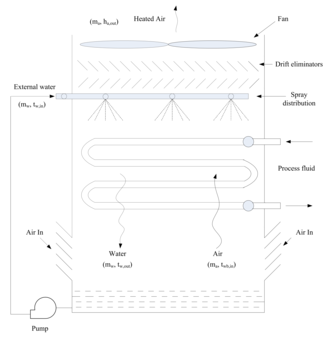
\includegraphics[width=0.9\textwidth, height=0.9\textheight, keepaspectratio=true]{media/image201.png}
\caption{Schematic diagram for evaporative fluid cooler \protect \label{fig:schematic-diagram-for-evaporative-fluid}}
\end{figure}

Where,

\begin{itemize}
\item
  h = Enthalpy (j/kg-K)
\item
  m = mass flow rate (kg/s)
\item
  Subscripts
\item
  a = air
\item
  w = water
\item
  wb = wet-bulb
\item
  in = inlet
\item
  out = outlet
\end{itemize}

\subsubsection{Inputs}\label{inputs-6-004}

\paragraph{Field: Name}\label{field-name-5-005}

This alpha field contains the identifying name for the fluid cooler.

\paragraph{Field: Water Inlet Node Name}\label{field-water-inlet-node-name-4}

This alpha field contains the identifying name for the fluid cooler's water inlet node.

\paragraph{Field: Water Outlet Node Name}\label{field-water-outlet-node-name-4}

This alpha field contains the identifying name for the fluid cooler's water outlet node.

\paragraph{Field: Design Air Flow Rate}\label{field-design-air-flow-rate-3}

This numeric field contains the design air flow rate induced by the fluid cooler fan in m\(^{3}\)/s. The field must contain a value greater than zero regardless of the fluid cooler performance input method. Alternately, this field can be autosized. See Engineering Reference document for autosizing calculations.

\paragraph{Field: Design Air Flow Rate Fan Power}\label{field-design-air-flow-rate-fan-power}

This numeric field contains the fan power (in watts) at the design air flow rate specified in the previous field. The field must contain a value greater than zero regardless of the fluid cooler performance input method. Alternately, this field can be autosized. See Engineering Reference document for autosizing calculations.

\paragraph{Field: Design Spray Water Flow Rate}\label{field-design-spray-water-flow-rate}

This numeric field contains the design spray water flow rate through the fluid cooler in m\(^{3}\)/s. A value greater than zero must be specified regardless of the performance input method,

\paragraph{Field: Performance Input Method}\label{field-performance-input-method-3}

This alpha field contains the method by which the user will specify fluid cooler performance: ``UFactorTimesAreaAndDesignWaterFlowRate'' or ``StandardDesignCapacity'' or ``UserSpecifiedDesignCapacity''.

\paragraph{Field: Outdoor Air Inlet Node Name}\label{field-outdoor-air-inlet-node-name-4}

This optional alpha field specifies the outdoor air node name used to define the conditions of the air entering the fluid cooler. If this field is left blank, the outdoor air conditions entering the fluid cooler are taken directly from the weather data. If this field is not blank, the node name specified must also be specified in an \hyperref[outdoorairnode]{OutdoorAir:Node} object where the height of the node is taken into consideration when calculating outdoor air conditions from the weather data. Alternately, the node name may be specified in an \hyperref[outdoorairnodelist]{OutdoorAir:NodeList} object where the outdoor air conditions are taken directly from the weather data.

\paragraph{Field: Heat Rejection Capacity and Nominal Capacity Sizing Ratio}\label{field-heat-rejection-capacity-and-nominal-capacity-sizing-ratio-3}

This numeric field contains the value for the ratio of actual tower heat rejection to nominal capacity.~ This ratio is defined at entering water at 35C (95F), leaving water at 29.4C (85F), entering air at 25.6C (78F) wetbulb and 35C (95F) drybulb temperatures. Historically this ratio has been set at 1.25 based on the assumption that the tower must dissipate 0.25 W of compressor power for every what of heat removed at the chiller evaporator.~ The default is 1.25.

\paragraph{Field: Standard Design Capacity}\label{field-standard-design-capacity}

This numeric input field contains the heat rejection capacity of the fluid cooler in watts, with entering water at 35C (95F), leaving water at 29.4C (85F), entering air at 25.6C (78F) wetbulb and 35C (95F) drybulb temperatures. The design water flow rate is assumed to be 5.382E-8 m\(^{3}\)/s per watt of nominal capacity (3 gpm/ton). 125\% of this capacity gives the actual fluid cooler heat rejection at these operating conditions (based on historical assumption that the evaporative fluid cooler must dissipate 0.25W of compressor heat for every watt of heat removed by the evaporator). This field is only used for performance input method = ''StandardDesignCapacity''. For other input methods this field is ignored. The standard conditions mentioned above for ``standard design capacity'' are already specified in the EnergyPlus. So the input fields such as design entering water temp., design entering air wet-bulb and dry-bulb temp. and design water flow rate, if provided in the input, will be ignored for the StandardDesignCapacity performance input method. Also, the standard conditions are for water as a fluid type so this performance input method can only be used with water as a fluid type (ref. \hyperref[condenserloop]{CondenserLoop} object).

\paragraph{Field: Design Air Flow Rate U-factor Times Area Value}\label{field-design-air-flow-rate-u-factor-times-area-value-1}

This numeric field contains the heat transfer coefficient-area product (UA) in watts per Kelvin corresponding to the design air and water flow rates specified above. If the input field ``Performance Input Method'' is specified as ``UFactorTimesAreaAndDesignWaterFlowRate'', then a UA value greater than zero but less than or equal to 300,000 must be defined, or the field can be autosized. If autosized, a Plant Sizing object must be defined and the design fluid cooler UA value is derived from the design load to be rejected by the condenser loop and the design loop delta T (Ref. Sizing and Input for Design Calculations and Component Autosizing sections), the fluid cooler inlet air dry-bulb and wetbulb temperature are taken from the input. This field is only used for performance input method = '' UFactorTimesAreaAndDesignWaterFlowRate''. For other performance input methods, this field is ignored.

\paragraph{Field: Design Water Flow Rate}\label{field-design-water-flow-rate-4}

This numeric field contains the design water flow rate through the fluid cooler in m\(^{3}\)/s. This value is the flow rate of the condenser loop water being cooled by the fluid cooler. This field is ignored for the ``StandardDesignCapacity'' performance input method. If autosized, a Plant Sizing object must be defined and the design water flow rate is derived from the design load to be rejected by the condenser loop and the design loop delta T (Ref. Sizing and Input for Design Calculations and Component Autosizing sections).

\paragraph{Field: User Specified Design Capacity}\label{field-user-specified-design-capacity}

This numeric input field contains the heat rejection capacity of the fluid cooler in watts. Design conditions for this capacity i.e.~entering air dry-bulb temperature, entering air wet-bulb temperature and entering water temperature must be provided in the input. Only used for Performance Input Method = UserSpecifiedDesignCapacity; for other performance input methods this field is ignored.

\paragraph{Field:Design Entering Water Temperature}\label{fielddesign-entering-water-temperature}

This numeric field contains entering water temperature at nominal conditions in degrees Celsius. The design entering water temperature must be greater than the design entering air temperature. Only used for Performance Input Method = UserSpecifiedDesignCapacity; for other performance input methods this field is ignored.

\paragraph{Field:Design Entering Air Temperature}\label{fielddesign-entering-air-temperature}

This numeric field contains entering air dry-bulb temperature at nominal conditions in degrees Celsius. The design entering air temperature must be greater than the design entering air wet-bulb temperature. Only used for Performance Input Method = UserSpecifiedDesignCapacity; for other performance input methods this field is ignored.

\paragraph{Field:Design Entering Air Wet-bulb Temperature}\label{fielddesign-entering-air-wet-bulb-temperature}

This numeric field contains entering air wetbulb temperature at nominal conditions in degrees Celsius. The design entering air wet-bulb temperature must be less than the design entering air (dry-bulb) temperature. Only used for Performance Input Method = UserSpecifiedDesignCapacity; for other performance input methods this field is ignored.

\paragraph{Field: Capacity Control}\label{field-capacity-control}

This alpha field contains the cooling capacity control for the evaporative fluid cooler. Two choices are available: FanCycling and FluidBypass. During part-load conditions, there are two ways to maintain the exiting water temperature at the setpoint: either cycling the evaporative fluid cooler fan, or bypassing portion of the evaporative fluid cooler water with a three-way valve. For FluidBypass, the evaporative fluid cooler fan still runs at full speed for the entire timestep, but only portion of the water flow goes through the evaporative fluid cooler media to get cooled while the remaining portion of the water flow gets bypassed. Two water flows then mix at the common water sump to meet the setpoint temperature.

\paragraph{Field: Sizing Factor}\label{field-sizing-factor-3}

This optional numeric field allows the user to specify a sizing factor for this component. The sizing factor is used when the component design inputs are autosized: the autosizing calculations are performed as usual and the results are multiplied by the sizing factor. Sizing factor allows the user to size a component to meet part of the design load while continuing to use the autosizing feature. For this component the inputs that would be altered by the sizing factor are:

1.~~ Design Water Flow Rate;

2.~~ Design Air Flow Rate;

3.~~ Fan Power at Design Air Flow Rate;

4.~~ U-Factor Times Area Value at Design Air Flow Rate;

Note that the U-Factor Times Area Value at Design Air Flow Rate is not multiplied by the Sizing Factor. Instead the design evaporative fluid cooler load is multiplied by the sizing factor and the design UA then calculated as usual.

\paragraph{Field: Evaporation Loss Mode}\label{field-evaporation-loss-mode-4}

This field is used to choose which method is used to model the amount of water evaporated by the evaporative fluid cooler. There are two options: LossFactor or SaturatedExit. The default is SaturatedExit. The user-defined loss factor is entered in the following field. By assuming that the air leaving the evaporative fluid cooler is saturated, the evaporation can be directly calculated using moist air engineering calculations with data available within the evaporative fluid cooler model (and does not require additional user input).

\paragraph{Field: Evaporation Loss Factor}\label{field-evaporation-loss-factor-4}

This field is used to specify the rate of water evaporated from the evaporative fluid cooler and lost to the outside air {[}percent/K{]}. This field is only used if the Evaporation Calculation Mode is set to LossFactor. The evaporation loss is then calculated as a fraction of the circulating condenser water flow and varies with the temperature change in the condenser water. The value entered here is in units of percent-per-kelvin. The evaporation rate will equal this value times each degree Kelvin of temperature drop in the condenser water. Empirical correlation is used to calculate default loss factor if it not explicitly specified in the input file.

\paragraph{Field: Drift Loss Percent}\label{field-drift-loss-percent-4}

This field is used to specify the rate of water lost to the exiting air as entrained droplets {[}\%{]}. The drift loss is a percent of the condenser water flow. Default value is under investigation for now cooling tower's evaporation loss factor is taken as default value.

\paragraph{Field: Blowdown Calculation Mode}\label{field-blowdown-calculation-mode-4}

This field specifies which method is used to determine blowdown rates. There two options ConcentrationRatio or ScheduledRate. The choice will determine which of the two models below is used. The default is ConcentrationRatio.

\paragraph{Field: Blowdown Concentration Ratio}\label{field-blowdown-concentration-ratio-4}

This field is used to dynamically adjust the rate of blowdown in the evaporative fluid cooler as a function of the rate of evaporation. Blowdown is water intentionally drained from the evaporative fluid cooler in order to offset the build up of solids in the water that would otherwise occur because of evaporation. The value entered here is dimensionless. It can be characterized as the ratio of solids in the blowdown water to solids in the make up water. Default value is under investigation for now cooling tower's evaporation loss factor is taken as default value.

\paragraph{Field: Blowdown Makeup Water Usage Schedule Name}\label{field-blowdown-makeup-water-usage-schedule-name-4}

This alpha field contains the name of the schedule used to define the amount of water (m3/s) flushed from the basin on a periodic basis to purge the evaporative fluid cooler of mineral scale build-up and other contaminants. This schedule is only used if the Blowdown Calculation Mode is set to ScheduledRate. The amount of water use due to blowdown depends on the makeup water quality and is specific to each geographical location. Default value is under investigation for now cooling tower's evaporation loss factor is taken as default value.This water usage is in addition to the amount of water lost to the atmosphere due to evaporation and/or drift. Since blowdown occurs when the basin water contaminant concentration is high, blowdown only occurs when the evaporative fluid cooler is active and water is flowing through the evaporative fluid cooler (regardless of the water usage defined by this schedule).

\paragraph{Field: Supply Water Storage Tank Name}\label{field-supply-water-storage-tank-name-4}

This field is optional. It is used to describe where the evaporative fluid cooler obtains water used for evaporative cooling. If blank or omitted, then the evaporative fluid cooler will obtain water directly from the mains. If the name of a \hyperref[waterusestorage]{WaterUse:Storage} object is used here, then the evaporative fluid cooler will obtain its water from that tank. If a tank is specified, the evaporative fluid cooler will attempt to obtain all the water it uses from the tank. However if the tank cannot provide all the water the evaporative fluid cooler needs, then the evaporative fluid cooler will still operate and obtain the rest of the water it needs from the mains (referred to as `Starved' water).

An IDF specification for this object is shown below:

\begin{lstlisting}

EvaporativeFluidCooler:SingleSpeed,
      Big EvaporativeFluidCooler,         !- Name
      Condenser EvaporativeFluidcooler Inlet Node,  !- Water Inlet Node Name
      Condenser EvaporativeFluidcooler Outlet Node,  !- Water Outlet Node Name
      3.02,                    !- Design Air Flow Rate {m3/s}
      2250,                    !- Design Air Flow Rate Fan Power {W}
      0.002208,                !- Design Spray Water Flow Rate {m3/s}
      UserSpecifiedDesignCapacity,                        !- Performance Input Method
      ,                        !- Outdoor Air Inlet Node Name
      1.25,                    !- Heat Rejection Capacity and Nominal Capacity Sizing Ratio
      ,                        !- Standard Design Capacity {W}
      ,                        !- Design Air Flow Rate U-factor Times Area Value {W/K}
      0.001703,                !- Design Water Flow Rate {m3/s}
      87921,                   !- User Specified Design Capacity {W}
      46.11,                   !- Design Entering Water Temperature {C}
      35,                      !- Design Entering Air Temperature {C}
      25.6;                    !- Design Entering Air Wet-bulb Temperature {C}
\end{lstlisting}

\subsubsection{Outputs}\label{outputs-6-001}

\begin{itemize}
\item
  HVAC,Average,Cooling Tower Fan Electricity Rate {[}W{]}
\item
  HVAC,Sum,Cooling Tower Fan Electricity Energy {[}J{]}
\item
  HVAC,Average,Cooling Tower Heat Transfer Rate {[}W{]}
\item
  HVAC,Average,Cooling Tower Inlet Temperature {[}C{]}
\item
  HVAC,Average,Cooling Tower Outlet Temperature {[}C{]}
\item
  HVAC,Average,Cooling Tower Mass Flow Rate {[}kg/s{]}
\item
  HVAC,Average,Cooling Tower Bypass Fraction {[]}
\item
  HVAC,Average,Cooling Tower Make Up Water Volume Flow Rate {[}m3/s{]}
\item
  HVAC,Sum,Cooling Tower Make Up Water Volume {[}m3{]}
\item
  HVAC,Average,Cooling Tower Water Evaporation Volume Flow Rate {[}m3/s{]}
\item
  HVAC,Sum,Cooling Tower Water Evaporation Volume {[}m3{]}
\item
  HVAC,Average,Cooling Tower Water Drift Volume Flow Rate {[}m3/s{]}
\item
  HVAC,Sum,Evaporative Fluid Cooler Water Drift {[}m3{]}
\item
  HVAC,Average,Cooling Tower Water Blowdown Volume Flow Rate {[}m3/s{]}
\item
  HVAC,Sum,Cooling Tower Water Blowdown Volume {[}m3{]}
\item
  HVAC,Sum,Cooling Tower Make Up Mains Water Volume {[}m3{]}
\end{itemize}

If Supply Water Storage Tank Name is specified:

\begin{itemize}
\item
  HVAC,Average,Cooling Tower Storage Tank Water Volume Flow Rate {[}m3/s{]}
\item
  HVAC,Sum,Cooling Tower Storage Tank Water Volume {[}m3{]}
\item
  HVAC,Average,Cooling Tower Starved Storage Tank Water Volume Flow Rate {[}m3/s{]}
\item
  HVAC,Sum,Cooling Tower Starved Storage Tank Water Volume {[}m3{]}
\end{itemize}

\paragraph{Cooling Tower Fan Electricity Rate {[}W{]}}\label{cooling-tower-fan-electric-power-w-4}

The average electric power consumption of the fluid cooler fan in Watts for the timestep being reported.

\paragraph{Cooling Tower Fan Electricity Energy {[}J{]}}\label{cooling-tower-fan-electric-energy-j-4}

Fan energy use in Joules.~ Consumption is metered on HeatRejection:Electricity, Electricity:Plant, and Electricity:Facility.

\paragraph{Cooling Tower Heat Transfer Rate {[}W{]}}\label{cooling-tower-heat-transfer-rate-w-4}

This is the average rate, in Watts, at which heat is removed from the condenser water loop by the fluid cooler for the time step being reported.

\paragraph{Cooling Tower Inlet Temperature {[}C{]}}\label{cooling-tower-inlet-temperature-c-4}

The fluid temperature at the fluid cooler inlet in degrees Celsius.

\paragraph{Cooling Tower Outlet Temperature {[}C{]}}\label{cooling-tower-outlet-temperature-c-4}

The fluid temperature at the fluid cooler outlet in degrees Celsius.

\paragraph{Cooling Tower Mass Flow Rate {[}kg/s{]}}\label{cooling-tower-mass-flow-rate-kgs-4}

The average fluid mass flow rate through the fluid cooler in kg/s for the time step being reported.

\paragraph{Cooling Tower Bypass Fraction {[]}}\label{cooling-tower-bypass-fraction-1}

This output is the average fluid bypass fraction for the time step being reported. See Capacity Control input field.

\paragraph{Cooling Tower Make Up Water Volume Flow Rate {[}m3/s{]}}\label{cooling-tower-make-up-water-volume-flow-rate-m3s-4}

\paragraph{Cooling Tower Make Up Water Volume {[}m3{]}}\label{cooling-tower-make-up-water-volume-m3-4}

These outputs are the external spray water consumed by the evaporative fluid cooler. This is the total of evaporation, drift, and blowdown.

\paragraph{Cooling Tower Water Evaporation Volume Flow Rate {[}m3/s{]}}\label{cooling-tower-water-evaporation-volume-flow-rate-m3s-4}

\paragraph{Cooling Tower Water Evaporation Volume {[}m3{]}}\label{cooling-tower-water-evaporation-volume-m3-4}

\paragraph{Cooling Tower Water Drift Volume Flow Rate {[}m3/s{]}}\label{cooling-tower-water-drift-volume-flow-rate-m3s-4}

\paragraph{Cooling Tower Water Drift Volume~ {[}m3{]}}\label{cooling-tower-water-drift-volume-m3-4}

\paragraph{Cooling Tower Water Blowdown Volume Flow Rate {[}m3/s{]}}\label{cooling-tower-water-blowdown-volume-flow-rate-m3s-4}

\paragraph{Cooling Tower Water Blowdown Volume {[}m3{]}}\label{cooling-tower-water-blowdown-volume-m3-4}

These outputs provide the breakdown of the different components of water use during fluid cooler operation.

\paragraph{Cooling Tower Make Up Mains Water Volume {[}m3{]}}\label{cooling-tower-make-up-mains-water-volume-m3-4}

The volume of make up water provided by the mains in cubic meters. If no Supply Water Storage Tank is specified, then all fluid cooler make up water is provided by the mains (same as Cooling Tower Make Up Water Volume). If a Supply Water Storage Tank is specified, then the make up from the mains only occurs when sufficient water supply is not available from the tank (same as Evaporative Fluid Cooler Water Starved by Storage Tank). This output variable is metered on HeatRejection:MainsWater, MainsWater:Plant and MainsWater:Facility.

\paragraph{Cooling Tower Storage Tank Water Volume Flow Rate {[}m3/s{]}}\label{cooling-tower-storage-tank-water-volume-flow-rate-m3s-4}

\paragraph{Cooling Tower Storage Tank Water Volume {[}m3{]}}\label{cooling-tower-storage-tank-water-volume-m3-4}

These are the rate and volume of water provided by the Supply Water Storage Tank.

\paragraph{Cooling Tower Starved Storage Tank Water Volume Flow Rate {[}m3/s{]}}\label{cooling-tower-starved-storage-tank-water-volume-flow-rate-m3s-4}

\paragraph{Cooling Tower Starved Storage Tank Water Volume {[}m3{]}}\label{cooling-tower-starved-storage-tank-water-volume-m3-4}

These are the rate and volume of water the Supply Water Storage Tank was not able to provide. The starved water is assumed to come from the mains. The fluid cooler's operation is not affected by a lack of storage tank water.

\subsection{EvaporativeFluidCooler:TwoSpeed}\label{evaporativefluidcoolertwospeed}

The two-speed evaporative fluid cooler is modeled in a similar fashion to the single-speed evaporative fluid cooler. The evaporative fluid cooler is modeled as a counter flow heat exchanger with two-speed fan (induced draft configuration. See schematic diagram in \hyperref[evaporativefluidcoolersinglespeed]{Evaporative\hyperref[fluidcoolersinglespeed]{FluidCooler:SingleSpeed}} section). The user must define fluid cooler performance via one of the three methods: design heat transfer coefficient-area product (UA) and design water flow rate, or standard fluid cooler design capacity at a specific rating point or design capacity at non standard conditions. Regardless of which method is chosen, the design airflow rate and corresponding fan power must be specified.

The evaporative fluid cooler seeks to maintain the temperature of the water exiting the evaporative fluid cooler at (or below) a set point. The set point schedule value is defined by the field ``Condenser Loop Temperature Setpoint Node Name or Reference'' for the \hyperref[condenserloop]{CondenserLoop} object. The model first checks to see whether inlet water temperature is at or below the set point. If so, then the fluid cooler fan is not turned on and all the flow goes through bypass. If the inlet water temperature is above the set point then the fluid cooler fan is turned on at low speed to reduce the exiting water temperature to the set point. If operating the fluid cooler fan at low speed does not reduce the exiting water temperature to the set point, then the fluid cooler fan is increased to its high speed.

The model assumes that part-load operation is represented by a simple linear interpolation between two steady-state regimes (i.e., fluid cooler fan at high speed for the entire simulation timestep and fluid cooler fan at low speed for the entire simulation timestep, or fluid cooler fan at low speed for the entire simulation timestep and fluid cooler fan off for the entire simulation timestep). Cyclic losses are not taken into account.

Evaporative fluid coolers consume water through evaporation, drift, and blowdown. The model can be used to predict water consumed by the evaporative fluid coolers. For this purpose, the last seven input fields can either be provided in the input or if nothing is specified then the default values for these fields will be used. These fields provide methods of controlling details of the water consumption calculations. The user can specify connections to the rest of the buildings water system by providing the name of a water storage tanks (i.e.~\hyperref[waterusestorage]{WaterUse:Storage} objects).

\subsubsection{Inputs}\label{inputs-7-004}

\paragraph{Field: Name}\label{field-name-6-004}

This alpha field contains the identifying name for the fluid cooler.

\paragraph{Field: WaterInlet Node Name}\label{field-waterinlet-node-name}

This alpha field contains the identifying name for the fluid cooler's water inlet node.

\paragraph{Field: Water Outlet Node Name}\label{field-water-outlet-node-name-5}

This alpha field contains the identifying name for the fluid cooler's water outlet node.

\paragraph{Field: High Fan Speed Air Flow Rate}\label{field-high-fan-speed-air-flow-rate-1}

This numeric field contains the fluid cooler air flow rate at high fan speed in m\(^{3}\)/s. A value greater than zero must be defined regardless of fluid cooler performance input method. Alternately, this field can be autosized. See Engineering Reference document for fluid cooler autosizing.

\paragraph{Field: High Fan Speed Fan Power}\label{field-high-fan-speed-fan-power}

This numeric field contains the fan power (in Watts) at the high-speed air flow rate specified in the previous field. A value greater than zero must be specified regardless of fluid cooler performance input method, or this field can be autosized. See Engineering Reference document for fluid cooler autosizing.

\paragraph{Field: Low Fan Speed Air Flow Rate}\label{field-low-fan-speed-air-flow-rate-1}

This numeric field contains the fluid cooler air flow rate at low fan speed in m\(^{3}\)/s. This value must be greater than zero, less than the value specified for the field ``Air Flow Rate at High Fan Speed''. This field may be autocalculated, in which case it is set to a fraction of the ``Air Flow Rate at High Fan Speed'' determined in the following field.

\paragraph{Field: Low Fan Speed Air Flow Rate Sizing Factor}\label{field-low-fan-speed-air-flow-rate-sizing-factor-1}

This numeric field contains the sizing factor for calculating the low fan speed air flow rate as a fraction of the high fan speed air flow rate.~ The default is 0.5.

\paragraph{Field: Low Fan Speed Fan Power}\label{field-low-fan-speed-fan-power-1}

This numeric field contains the fan power (in Watts) at the low-speed air flow rate specified in the previous field. This value must be specified greater than zero or the field may be autocalculated, in which case it is set to a fraction of the ``Fan Power at High Fan Speed'' determined in the following field.

\paragraph{Field: Low Fan Speed Fan Power Sizing Factor}\label{field-low-fan-speed-fan-power-sizing-factor-1}

This numeric field contains the sizing factor for calculating the low fan speed fan power as a fraction of the high fan speed fan power. ~The default is 0.16.

\paragraph{Field: Design Spray Water Flow Rate}\label{field-design-spray-water-flow-rate-1}

This numeric field contains the design spray water flow rate through the fluid cooler in m\(^{3}\)/s. This input field must be specified for all the performance input methods.

\paragraph{Field: Performance Input Method}\label{field-performance-input-method-4}

This alpha field contains the method by which the user will specify fluid cooler performance: ``UFactorTimesAreaAndDesignWaterFlowRate'' or ``StandardDesignCapacity'' or ``UserSpecifiedDesignCapacity''.

\paragraph{Field: Outdoor Air Inlet Node Name}\label{field-outdoor-air-inlet-node-name-5}

This optional alpha field specifies the outdoor air node name used to define the conditions of the air entering the fluid cooler. If this field is left blank, the outdoor air conditions entering the fluid cooler are taken directly from the weather data. If this field is not blank, the node name specified must also be specified in an \hyperref[outdoorairnode]{OutdoorAir:Node} object where the height of the node is taken into consideration when calculating outdoor air conditions from the weather data. Alternately, the node name may be specified in an \hyperref[outdoorairnodelist]{OutdoorAir:NodeList} object where the outdoor air conditions are taken directly from the weather data.

\paragraph{Field: Heat Rejection Capacity and Nominal Capacity Sizing Ratio}\label{field-heat-rejection-capacity-and-nominal-capacity-sizing-ratio-4}

This numeric field contains the value for the ratio of actual tower heat rejection to nominal capacity.~ This ratio is defined at entering water at 35C (95F), leaving water at 29.4C (85F), entering air at 25.6C (78F) wetbulb and 35C (95F) drybulb temperatures. Historically this ratio has been set at 1.25 based on the assumption that the tower must dissipate 0.25 W of compressor power for every what of heat removed at the chiller evaporator.~ The default is 1.25.

\paragraph{Field: High Speed Standard Design Capacity}\label{field-high-speed-standard-design-capacity}

This numeric input field contains the heat rejection capacity of the fluid cooler in watts, with entering water at 35C (95F), leaving water at 29.4C (85F), entering air at 25.6C (78F) wetbulb and 35C (95F) drybulb temperatures. The design water flow rate is assumed to be 5.382E-8 m\(^{3}\)/s per watt of nominal capacity (3 gpm/ton). The Heat Rejection Capacity and Nominal Capacity Sizing Ratio set in the previous field is applied to this capacity to give the actual fluid cooler heat rejection at these operating conditions. This field is only used for performance input method = ''StandardDesignCapacity''. For other input methods this field is ignored. The standard conditions mentioned above for ``standard design capacity'' are already specified in the EnergyPlus. So the input fields such as design entering water temp., design entering air wet-bulb and dry-bulb temp. and design water flow rate, if provided in the input, will be ignored for the StandardDesignCapacity performance input method. Also, the standard conditions are for water as a fluid type so this performance input method can only be used with water as a fluid type (ref. \hyperref[condenserloop]{CondenserLoop} object).

\paragraph{Field: Low Speed Standard Design Capacity}\label{field-low-speed-standard-design-capacity}

This numeric input field contains the heat rejection capacity of the fluid cooler in watts, with entering water at 35C (95F), leaving water at 29.4C (85F), entering air at 25.6C (78F) wetbulb and 35C (95F) drybulb temperatures. The design water flow rate is assumed to be 5.382E-8 m\(^{3}\)/s per watt of nominal capacity (3 gpm/ton). The Heat Rejection Capacity and Nominal Capacity Sizing Ratio is applied to this capacity to give the actual fluid cooler heat rejection at these operating conditions. This field is only used for performance input method = ''StandardDesignCapacity''. For other input methods this field is ignored. The standard conditions mentioned above for ``standard design capacity'' are already specified in the EnergyPlus. So the input fields such as design entering water temp., design entering air wet-bulb and dry-bulb temp. and design water flow rate, if provided in the input, will be ignored for the StandardDesignCapacity performance input method. Also, the standard conditions are for water as a fluid type so this performance input method can only be used with water as a fluid type (ref. \hyperref[condenserloop]{CondenserLoop} object). The value specified for this field must be greater than zero but less than the value specified for the field ``High-Speed Standard Design Capacity''. This field may be autocalculated, in which case it is set to a fraction of the High-Speed Standard Design Capacity determined in the following field.

\paragraph{Field: Low Speed Standard Capacity Sizing Factor}\label{field-low-speed-standard-capacity-sizing-factor}

This numeric field contains the sizing factor to use when calculating the Low Speed Standard Design Capacity.~ The default is 0.5.

\paragraph{Field: High Fan Speed U-factor Times Area Value}\label{field-high-fan-speed-u-factor-times-area-value-1}

This numeric field contains the heat transfer coefficient-area product (UA) in watts per Kelvin corresponding to the high speed design air and water flow rates specified above. If the input field ``Performance Input Method'' is specified as ``UFactorTimesAreaAndDesignWaterFlowRate'', then a UA value greater than zero but less than or equal to 2,100,000 must be defined, or the field can be autosized. If autosized, a Plant Sizing object must be defined and the design fluid cooler UA value is derived from the design load to be rejected by the condenser loop and the design loop delta T (Ref. Sizing and Input for Design Calculations and Component Autosizing sections), the fluid cooler inlet air dry-bulb and wetbulb temperature are taken from the input. This field is only used for performance input method = '' UFactorTimesAreaAndDesignWaterFlowRate''. For other input methods this field is ignored.

\paragraph{Field: Low Fan Speed U-factor Times Area Value}\label{field-low-fan-speed-u-factor-times-area-value-1}

This numeric field contains the heat transfer coefficient-area product (UA) in watts per degree Kelvin corresponding to the low speed design air and water flow rates specified above. If the input field ``Performance Input Method'' is specified as ``UFactorTimesAreaAndDesignWaterFlowRate'', then a UA value greater than zero but less than or equal to 300,000 and less than the value specified for the field ``U-Factor Times Area Value at High Fan Speed'' must be defined. This field may be autocalculated, in which case it is set to a factor of the ``U-Factor Times Area Value at High Fan Speed'' determined in the following field. This field is only used for performance input method = '' UFactorTimesAreaAndDesignWaterFlowRate''. For other input methods this field is ignored.

\paragraph{Field: Low Fan Speed U-Factor Times Area Sizing Factor}\label{field-low-fan-speed-u-factor-times-area-sizing-factor-1}

This field contains the sizing factor to use when calculating the Low Fan Speed U-Factor Times Area Value.~ The default is 0.6.

\paragraph{Field: Design Water Flow Rate}\label{field-design-water-flow-rate-5}

This numeric field contains the design water flow rate through the fluid cooler in m\(^{3}\)/s. This value is the flow rate of the condenser loop water being cooled by the fluid cooler. This field is ignored for the ``StandardDesignCapacity'' performance input method. If autosized, a Plant Sizing object must be defined and the design water flow rate is derived from the design load to be rejected by the condenser loop and the design loop delta T (Ref. Sizing and Input for Design Calculations and Component Autosizing sections).

\paragraph{Field: High Speed User Specified Design Capacity}\label{field-high-speed-user-specified-design-capacity}

This numeric input field contains the heat rejection capacity of the fluid cooler in watts. Design conditions for this capacity i.e.~entering air dry-bulb temperature, entering air wet-bulb temperature and entering water temperature must be provided in the input. Only used for Performance Input Method = UserSpecifiedDesignCapacity; for other performance input methods this field is ignored.

\paragraph{Field: Low Speed User Specified Design Capacity}\label{field-low-speed-user-specified-design-capacity}

This numeric input field contains the heat rejection capacity of the fluid cooler in watts. Design conditions for this capacity i.e.~entering air dry-bulb temperature, entering air wet-bulb temperature and entering water temperature must be provided in the input. Only used for Performance Input Method = UserSpecifiedDesignCapacity; for other performance input methods this field is ignored. This field may be autocalculated, in which case it is set to a fraction of the ``High Speed User Specified Design Capacity'' determined in the following field.

\paragraph{Field: Low Speed User Specified Design Capacity Sizing Factor}\label{field-low-speed-user-specified-design-capacity-sizing-factor}

This field contains the sizing factor to use when calculating the Low-Speed User Specified Design Capacity.~ The default is 0.5.

\paragraph{Field:Design Entering Water Temperature}\label{fielddesign-entering-water-temperature-1}

This numeric field contains entering water temperature at nominal conditions in degrees Celsius. The design entering water temperature must be greater than the design entering air temperature. Only used for Performance Input Method = UserSpecifiedDesignCapacity; for other performance input methods this field is ignored.

\paragraph{Field:Design Entering Air Temperature}\label{fielddesign-entering-air-temperature-1}

This numeric field contains entering air dry-bulb temperature at nominal conditions in degrees Celsius. The design entering air temperature must be greater than the design entering air wet-bulb temperature. Only used for Performance Input Method = UserSpecifiedDesignCapacity; for other performance input methods this field is ignored.

\paragraph{Field:Design Entering Air Wet-bulb Temperature}\label{fielddesign-entering-air-wet-bulb-temperature-1}

This numeric field contains entering air wetbulb temperature at nominal conditions in degrees Celsius. The design entering air wet-bulb temperature must be less than the design entering air (dry-bulb) temperature. Only used for Performance Input Method = UserSpecifiedDesignCapacity; for other performance input methods this field is ignored.

\paragraph{Field: High Speed Sizing Factor}\label{field-high-speed-sizing-factor}

This optional numeric field allows the user to specify a sizing factor for this component. The sizing factor is used when the component design inputs are autosized: the autosizing calculations are performed as usual and the results are multiplied by the sizing factor. Sizing factor allows the user to size a component to meet part of the design load while continuing to use the autosizing feature. For this component the inputs that would be altered by the sizing factor are:

1.~~~~Design Water Flow Rate;

2.~~~~Air Flow Rate at High Fan Speed;

3.~~~~Fan Power at High Fan Speed;

4.~~~~U-Factor Times Area Value at High Fan Speed;

5.~~~~Air Flow Rate at Low Fan Speed;

6.~~~~Fan Power at Low Fan Speed;

7.~~~~U-Factor Times Area Value at Low Fan Speed;

Note that the U-Factor Times Area Value at High Fan Speed is not multiplied by the Sizing Factor. Instead the design evaporative fluid cooler load is multiplied by the sizing factor and the design UA then calculated as usual. The U-Factor Times Area Value at Low Fan Speed is set to Low Fan Speed U-Factor Times Area Sizing Factor times the full load design UA.

\paragraph{Field: Evaporation Loss Mode}\label{field-evaporation-loss-mode-5}

This field is used to choose which method is used to model the amount of water evaporated by the evaporative fluid cooler. There are two options: LossFactor or SaturatedExit. The default is SaturatedExit. The user-defined loss factor is entered in the following field. By assuming that the air leaving the evaporative fluid cooler is saturated, the evaporation can be directly calculated using moist air engineering calculations with data available within the evaporative fluid cooler model (and does not require additional user input).

\paragraph{Field: Evaporation Loss Factor}\label{field-evaporation-loss-factor-5}

This field is used to specify the rate of water evaporated from the evaporative fluid cooler and lost to the outside air {[}percent/K{]}. This field is only used if the Evaporation Calculation Mode is set to LossFactor. The evaporation loss is then calculated as a fraction of the circulating condenser water flow and varies with the temperature change in the condenser water. The value entered here is in units of percent-per-kelvin. The evaporation rate will equal this value times each degree Kelvin of temperature drop in the condenser water. Empirical correlation is used to calculate default loss factor if it not explicitly specified in the input file.

\paragraph{Field: Drift Loss Percent}\label{field-drift-loss-percent-5}

This field is used to specify the rate of water lost to the exiting air as entrained droplets {[}\%{]}. The drift loss is a percent of the condenser water flow. Default value is under investigation for now cooling tower's evaporation loss factor is taken as default value.

\paragraph{Field: Blowdown Calculation Mode}\label{field-blowdown-calculation-mode-5}

This field specifies which method is used to determine blowdown rates. There two options ConcentrationRatio or ScheduledRate. The choice will determine which of the two models below is used. The default is ConcentrationRatio.

\paragraph{Field: Blowdown Concentration Ratio}\label{field-blowdown-concentration-ratio-5}

This field is used to dynamically adjust the rate of blowdown in the evaporative fluid cooler as a function of the rate of evaporation. Blowdown is water intentionally drained from the evaporative fluid cooler in order to offset the build up of solids in the water that would otherwise occur because of evaporation. The value entered here is dimensionless. It can be characterized as the ratio of solids in the blowdown water to solids in the make up water. Default value is under investigation for now cooling tower's evaporation loss factor is taken as default value.

\paragraph{Field: Blowdown Makeup Water Usage Schedule Name}\label{field-blowdown-makeup-water-usage-schedule-name-5}

This alpha field contains the name of the schedule used to define the amount of water (m3/s) flushed from the basin on a periodic basis to purge the evaporative fluid cooler of mineral scale build-up and other contaminants. This schedule is only used if the Blowdown Calculation Mode is set to ScheduledRate. The amount of water use due to blowdown depends on the makeup water quality and is specific to each geographical location. Default value is under investigation for now cooling tower's evaporation loss factor is taken as default value.This water usage is in addition to the amount of water lost to the atmosphere due to evaporation and/or drift. Since blowdown occurs when the basin water contaminant concentration is high, blowdown only occurs when the evaporative fluid cooler is active and water is flowing through the evaporative fluid cooler (regardless of the water usage defined by this schedule).

\paragraph{Field: Supply Water Storage Tank Name}\label{field-supply-water-storage-tank-name-5}

This field is optional. It is used to describe where the evaporative fluid cooler obtains water used for evaporative cooling. If blank or omitted, then the evaporative fluid cooler will obtain water directly from the mains. If the name of a \hyperref[waterusestorage]{WaterUse:Storage} object is used here, then the evaporative fluid cooler will obtain its water from that tank. If a tank is specified, the evaporative fluid cooler will attempt to obtain all the water it uses from the tank. However if the tank cannot provide all the water the evaporative fluid cooler needs, then the evaporative fluid cooler will still operate and obtain the rest of the water it needs from the mains (referred to as `Starved' water).

Examples of an IDF specification for this object are shown below:

\begin{lstlisting}

EvaporativeFluidCooler:TwoSpeed,
      Big EvaporativeFluidCooler,         !- Name
      Condenser EvaporativeFluidcooler Inlet Node,  !- Water Inlet Node Name
      Condenser EvaporativeFluidcooler Outlet Node,  !- Water Outlet Node Name
      9.911,                   !- High Fan Speed Air Flow Rate {m3/s}
      autosize,                !- High Fan Speed Fan Power {W}
      4.911,                   !- Low Fan Speed Air Flow Rate {m3/s}
      0.5,                     !- Low Fan Speed Air Flow Rate Sizing Factor
      autosize,                !- Low Fan Speed Fan Power {W}
      0.16,                    !- Low Fan Speed Fan Power Sizing Factor
      0.002208,                !- Design Spray Water Flow Rate {m3/s}
      UserSpecifiedDesignCapacity,    !- Performance Input Method
      ,                        !- Outdoor Air Inlet Node Name
      1.25,                    !- Heat Rejection Capacity and Nominal Capacity Sizing Ratio
      ,                        !- High Speed Standard Design Capacity {W}
      ,                        !- Low Speed Standard Design Capacity {W}
      0.5,                     !- Low Speed Standard Capacity Sizing Factor
      ,                        !- High Fan Speed U-factor Times Area Value  {W/K}
      ,                        !- Low Fan Speed U-factor Times Area Value  {W/K}
      0.6,                     !- Low Fan Speed U-Factor Times Area Sizing Factor
      0.001703,                !- Design Water Flow Rate {m3/s}
      87921,                   !- High Speed User Specified Design Capacity {W}
      47921,                   !- Low Speed User Specified Design Capacity {W}
      0.5,                     !- Low Speed User Specified Design Capacity Sizing Factor
      46.11,                   !- Design Entering Water Temperature {C}
      35,                      !- Design Entering Air Temperature {C}
      25.6;                    !- Design Entering Air Wet-bulb Temperature {C}
\end{lstlisting}

\subsubsection{Outputs}\label{outputs-7-001}

\begin{itemize}
\item
  HVAC,Average,Cooling Tower Fan Electricity Rate {[}W{]}
\item
  HVAC,Sum,Cooling Tower Fan Electricity Energy {[}J{]}
\item
  HVAC,Average,Cooling Tower Heat Transfer Rate {[}W{]}
\item
  HVAC,Average,Cooling Tower Inlet Temperature {[}C{]}
\item
  HVAC,Average,Cooling Tower Outlet Temperature {[}C{]}
\item
  HVAC,Average,Cooling Tower Mass Flow Rate {[}kg/s{]}
\item
  HVAC,Average,Cooling Tower Make Up Water Volume Flow Rate {[}m3/s{]}
\item
  HVAC,Sum,Cooling Tower Make Up Water Volume {[}m3{]}
\item
  HVAC,Average,Cooling Tower Water Evaporation Volume Flow Rate {[}m3/s{]}
\item
  HVAC,Sum,Cooling Tower Water Evaporation Volume {[}m3{]}
\item
  HVAC,Average,Cooling Tower Water Drift Volume Flow Rate {[}m3/s{]}
\item
  HVAC,Sum,Cooling Tower Water Drift Volume {[}m3{]}
\item
  HVAC,Average,Cooling Tower Water Blowdown Volume Flow Rate {[}m3/s{]}
\item
  HVAC,Sum,Cooling Tower Water Blowdown Volume {[}m3{]}
\item
  HVAC,Sum,Cooling Tower Make Up Mains Water Volume {[}m3{]}
\end{itemize}

If Supply Water Storage Tank Name is specified:

\begin{itemize}
\item
  HVAC,Average,Cooling Tower Storage Tank Water Volume Flow Rate {[}m3/s{]}
\item
  HVAC,Sum,Cooling Tower Storage Tank Water Volume {[}m3{]}
\item
  HVAC,Average,Cooling Tower Starved Storage Tank Water Volume Flow Rate {[}m3/s{]}
\item
  HVAC,Sum,Cooling Tower Starved Storage Tank Water Volume {[}m3{]}
\end{itemize}

\paragraph{Cooling Tower Fan Electricity Rate {[}W{]}}\label{cooling-tower-fan-electric-power-w-5}

The average electric power consumption of the fluid cooler fan in Watts for the timestep being reported.

\paragraph{Cooling Tower Fan Electricity Energy {[}J{]}}\label{cooling-tower-fan-electric-energy-j-5}

Fan energy use in Joules.~ Consumption is metered on HeatRejection:Electricity, Electricity:Plant, and Electricity:Facility.

\paragraph{Cooling Tower Heat Transfer Rate {[}W{]}}\label{cooling-tower-heat-transfer-rate-w-5}

This is the average rate, in Watts, at which heat is removed from the condenser water loop by the fluid cooler for the time step being reported.

\paragraph{Cooling Tower Inlet Temperature {[}C{]}}\label{cooling-tower-inlet-temperature-c-5}

The fluid temperature at the fluid cooler inlet in degrees Celsius.

\paragraph{Cooling Tower Outlet Temperature {[}C{]}}\label{cooling-tower-outlet-temperature-c-5}

The fluid temperature at the fluid cooler outlet in degrees Celsius.

\paragraph{Cooling Tower Mass Flow Rate {[}kg/s{]}}\label{cooling-tower-mass-flow-rate-kgs-5}

The average fluid mass flow rate through the fluid cooler in kg/s for the time step being reported.

\paragraph{Cooling Tower Make Up Water Volume Flow Rate {[}m3/s{]}}\label{cooling-tower-make-up-water-volume-flow-rate-m3s-5}

\paragraph{Cooling Tower Make Up Water Volume {[}m3{]}}\label{cooling-tower-make-up-water-volume-m3-5}

These outputs are the external spray water consumed by the evaporative fluid cooler. This is the total of evaporation, drift, and blowdown.

\paragraph{Cooling Tower Water Evaporation Volume Flow Rate {[}m3/s{]}}\label{cooling-tower-water-evaporation-volume-flow-rate-m3s-5}

\paragraph{Cooling Tower Water Evaporation Volume {[}m3{]}}\label{cooling-tower-water-evaporation-volume-m3-5}

\paragraph{Cooling Tower Water Drift Volume Flow Rate {[}m3/s{]}}\label{cooling-tower-water-drift-volume-flow-rate-m3s-5}

\paragraph{Cooling Tower Water Drift Volume {[}m3{]}}\label{cooling-tower-water-drift-volume-m3-5}

\paragraph{Cooling Tower Water Blowdown Volume Flow Rate {[}m3/s{]}}\label{cooling-tower-water-blowdown-volume-flow-rate-m3s-5}

\paragraph{Cooling Tower Water Blowdown Volume {[}m3{]}}\label{cooling-tower-water-blowdown-volume-m3-5}

These outputs provide the breakdown of the different components of water use during fluid cooler operation.

\paragraph{Cooling Tower Make Up Mains Water Volume {[}m3{]}}\label{cooling-tower-make-up-mains-water-volume-m3-5}

The volume of make up water provided by the mains in cubic meters. If no Supply Water Storage Tank is specified, then all fluid cooler make up water is provided by the mains (same as Cooling Tower Make Up Water Volume). If a Supply Water Storage Tank is specified, then the make up from the mains only occurs when sufficient water supply is not available from the tank (same as Cooling Tower Starved Storage Tank Water Volume). This output variable is metered on HeatRejection:MainsWater, MainsWater:Plant and MainsWater:Facility.

\paragraph{Cooling Tower Storage Tank Water Volume Flow Rate {[}m3/s{]}}\label{cooling-tower-storage-tank-water-volume-flow-rate-m3s-5}

\paragraph{Cooling Tower Storage Tank Water Volume {[}m3{]}}\label{cooling-tower-storage-tank-water-volume-m3-5}

These are the rate and volume of water provided by the Supply Water Storage Tank.

\paragraph{Cooling Tower Starved Storage Tank Water Volume Flow Rate {[}m3/s{]}}\label{cooling-tower-starved-storage-tank-water-volume-flow-rate-m3s-5}

\paragraph{Cooling Tower Starved Storage Tank Water Volume {[}m3{]}}\label{cooling-tower-starved-storage-tank-water-volume-m3-5}

These are the rate and volume of water the Supply Water Storage Tank was not able to provide. The starved water is assumed to come from the mains. The fluid cooler's operation is not affected by a lack of storage tank water.

\subsection{FluidCooler:SingleSpeed}\label{fluidcoolersinglespeed}

Fluid coolers are components that may be assigned to condenser loops. The Fluid cooler is modeled as a cross flow heat exchanger (both streams unmixed) with single-speed fans (induced draft configuration). The user must define fluid cooler performance via one of the two methods: design heat transfer coefficient-area product (UA) and design water flow rate, or nominal fluid cooler capacity at a specific rating point. Regardless of which method is chosen, the design airflow rate and corresponding fan power must be specified.

The fluid cooler seeks to maintain the temperature of the water exiting the fluid cooler at (or below) a set point. The set point schedule value is defined by the field ``Condenser Loop Temperature Setpoint Node Name or Reference'' for the \hyperref[condenserloop]{CondenserLoop} object. The model assumes that part-load operation is represented by a simple linear interpolation between two steady-state regimes (i.e., fluid cooler fan on for the entire simulation timestep and fluid cooler fan off for the entire simulation timestep). Cyclic losses are not taken into account.

\subsubsection{Inputs}\label{inputs-8-003}

\paragraph{Field: Name}\label{field-name-7-003}

This alpha field contains the identifying name for the Fluid Cooler.

\paragraph{Field: Water Inlet Node Name}\label{field-water-inlet-node-name-5}

This alpha field contains the identifying name for the Fluid Cooler's water inlet node.

\paragraph{Field: Water Outlet Node Name}\label{field-water-outlet-node-name-6}

This alpha field contains the identifying name for the Fluid Cooler's water outlet node.

\paragraph{Field: Performance Input Method}\label{field-performance-input-method-5}

This alpha field contains the method by which the user will specify fluid cooler performance: ``UFactorTimesAreaAndDesignWaterFlowRate'' or ``NominalCapacity''.

\paragraph{Field: Design Air Flow Rate U-factor Times Area Value}\label{field-design-air-flow-rate-u-factor-times-area-value-2}

This numeric field contains the heat transfer coefficient-area product (UA) in watts per Kelvin corresponding to the design air and water flow rates specified above. If the input field ``Performance Input Method'' is specified as ``UFactorTimesAreaAndDesignWaterFlowRate'', then a UA value greater than zero but less than or equal to 300,000 must be defined, or the field can be autosized. If autosized, a Plant Sizing object must be defined and the design fluid cooler UA value is derived from the design load to be rejected by the condenser loop and the design loop delta T (Ref. Sizing and Input for Design Calculations and Component Autosizing sections), the fluid cooler inlet air dry-bulb and wetbulb temperature are taken from the input. If ``Performance Input Method'' is specified as ``NominalCapacity'', then this field must be left blank since the model automatically calculates the fluid cooler UA based on the fluid cooler capacity and nominal conditions specified in input file.

\paragraph{Field: Nominal Capacity}\label{field-nominal-capacity-2}

This numeric input field contains the ``nominal'' heat rejection capacity of the fluid cooler in watts, Nominal conditions i.e.~entering air dry-bulb temperature, entering air wet-bulb temperature and Entering water temperature should be provided in the input.

\paragraph{Field:Design Entering Water Temperature}\label{fielddesign-entering-water-temperature-2}

This numeric field contains entering water temperature at nominal conditions in degrees Celsius. This field must be specified for both the performance input methods. The design entering water temperature must be greater than the design entering air temperature.

\paragraph{Field:Design Entering Air Temperature}\label{fielddesign-entering-air-temperature-2}

This numeric field contains entering air dry-bulb temperature at nominal conditions in degrees Celsius. This field must be specified for both the performance input methods. The design entering air temperature must be greater than the design entering air wet-bulb temperature.

\paragraph{Field:Design Entering Air Wet-bulb Temperature}\label{fielddesign-entering-air-wet-bulb-temperature-2}

This numeric field contains entering air wetbulb temperature at nominal conditions in degrees Celsius. This field must be specified for both the performance input methods. The design entering air wet-bulb temperature must be less than the design entering air (dry-bulb) temperature.

\paragraph{Field: Design Water Flow Rate}\label{field-design-water-flow-rate-6}

This numeric field contains the design water flow rate through the fluid cooler in m\(^{3}\)/s. This value is the flow rate of the condenser loop water being cooled by the fluid cooler. A water flow rate greater than zero must be defined or the field can be autosized. If autosized, a Plant Sizing object must be defined and the design water flow rate is derived from the design load to be rejected by the condenser loop and the design loop delta T (Ref. Sizing and Input for Design Calculations and Component Autosizing sections).

\paragraph{Field: Design Air Flow Rate}\label{field-design-air-flow-rate-4}

This numeric field contains the design air flow rate induced by the fluid cooler fan in m\(^{3}\)/s. A value greater than zero must be defined regardless of the fluid cooler performance input method. Alternately, this field can be autosized. See Engineering Reference document for fluid cooler autosizing.

\paragraph{Field: Design Air Flow Rate Fan Power}\label{field-design-air-flow-rate-fan-power-1}

This numeric field contains the fan power (in watts) at the design air flow rate specified in the previous field. A value greater than zero must be specified regardless of the performance input method, or this field can be autosized. See Engineering ref. for fluid cooler autosizing.

\paragraph{Field: Outdoor Air Inlet Node Name}\label{field-outdoor-air-inlet-node-name-6}

This optional alpha field specifies the outdoor air node name used to define the conditions of the air entering the fluid cooler. If this field is left blank, the outdoor air conditions entering the fluid cooler are taken directly from the weather data. If this field is not blank, the node name specified must also be specified in an \hyperref[outdoorairnode]{OutdoorAir:Node} object where the height of the node is taken into consideration when calculating outdoor air conditions from the weather data. Alternately, the node name may be specified in an \hyperref[outdoorairnodelist]{OutdoorAir:NodeList} object where the outdoor air conditions are taken directly from the weather data.

An IDF specification for this object is shown below:

\begin{lstlisting}

FluidCooler:SingleSpeed,
      Big FLUIDCOOLER1,              !- Name
      Condenser FLUIDCOOLER 1 Inlet Node,  !- Water Inlet Node Name
      Condenser FLUIDCOOLER 1 Outlet Node, !- Water Outlet Node Name
      NominalCapacity,        !- Performance Input Method
      ,                       !- Design Air Flow Rate U-factor Times Area Value {W/K}
      58601.,                 !- Nominal Capacity {W}
      51.67,                  !- Design Entering Water Temperature {C}
      35,                     !- Design Entering Air Temperature {C}
      25.6,                   !- Design Entering Air Wetbulb Temperature {C}
      0.001388,               !- Design Water Flow Rate{m3/s}
      9.911,                  !- Design Air Flow Rate {m3/s}
      Autosize;               !- Design Air Flow Rate Fan Power {W}
\end{lstlisting}

\subsubsection{Outputs}\label{outputs-8-000}

\begin{itemize}
\item
  HVAC,Average,Cooling Tower Fan Electricity Rate {[}W{]}
\item
  HVAC,Sum,Cooling Tower Fan Electricity Energy {[}J{]}
\item
  Zone,Meter,HeatRejection:Electricity {[}J{]}
\item
  HVAC,Average,Cooling Tower Heat Transfer Rate {[}W{]}
\item
  HVAC,Average, Cooling Tower Inlet Temperature {[}C{]}
\item
  HVAC,Average, Cooling Tower Outlet Temperature {[}C{]}
\item
  HVAC,Average,Cooling Tower Mass Flow Rate {[}kg/s{]}
\end{itemize}

\paragraph{Cooling Tower Fan Electricity Rate {[}W{]}}\label{cooling-tower-fan-electric-power-w-6}

The electric power consumption of the fluid cooler fans.

\paragraph{Cooling Tower Fan Electricity Energy {[}J{]}}\label{cooling-tower-fan-electric-energy-j-6}

Fan energy use.~ Consumption is metered on HeatRejection:Electricity, Electricity:Plant, and Electricity:Facility.

\paragraph{Cooling Tower Heat Transfer Rate {[}W{]}}\label{cooling-tower-heat-transfer-rate-w-6}

This is the rate at which heat is removed from the condenser water loop by the fluid cooler.

\paragraph{Cooling Tower Inlet Temperature {[}C{]}}\label{cooling-tower-inlet-temperature-c-6}

The loop temperature at the fluid cooler inlet.

\paragraph{Cooling Tower Outlet Temperature {[}C{]}}\label{cooling-tower-outlet-temperature-c-6}

The loop temperature at the fluid cooler outlet.

\paragraph{Cooling Tower Mass Flow Rate {[}kg/s{]}}\label{cooling-tower-mass-flow-rate-kgs-6}

The loop mass flow rate of the circulating condenser water loop.

\subsection{FluidCooler:TwoSpeed}\label{fluidcoolertwospeed}

The two-speed fluid cooler is modeled in a similar fashion to the single-speed fluid cooler. The fluid cooler is modeled as a cross flow heat exchanger (both stream unmixed) with~ two-speed fans (induced draft configuration). The user must define fluid cooler performance via one of two methods: heat transfer coefficient-area product (UA) and design water flow rate, or nominal fluid cooler capacity at a specific rating point. Regardless of which method is chosen, the airflow rate and corresponding fan power at both high and low fan speed must be specified. The Fluid Cooler seeks to maintain the temperature of the water exiting the Fluid Cooler at (or below) a set point. The set point schedule is defined by the field ``Condenser Loop Temperature Setpoint Node Name or Reference'' for the \hyperref[condenserloop]{CondenserLoop} object. The model first runs at low speed and calculates the fluid cooler exiting water temperature. If the exiting water temperature based on ``low speed'' is at or below the set point, then the fluid cooler fan runs at this speed or below this speed. If the exiting water temperature remains above the set point after ``low speed'' is modeled, then the fluid cooler fan runs at high speed to reduce the exiting water temperature.

The model assumes that part-load operation is represented by a simple linear interpolation between two steady-state regimes (i.e., fluid cooler fan at high speed for the entire simulation timestep and fluid cooler fan at low speed for the entire simulation timestep,). Cyclic losses are not taken into account.

\subsubsection{Inputs}\label{inputs-9-003}

\paragraph{Field: Name}\label{field-name-8-003}

This alpha field contains the identifying name for the fluid cooler.

\paragraph{Field: Water Inlet Node Name}\label{field-water-inlet-node-name-6}

This alpha field contains the identifying name for the fluid cooler's water inlet node.

\paragraph{Field: Water Outlet Node Name}\label{field-water-outlet-node-name-7}

This alpha field contains the identifying name for the fluid cooler's water outlet node.

\paragraph{Field: Performance Input Method}\label{field-performance-input-method-6}

This alpha field contains the method by which the user will specify fluid cooler performance: ``UFactorTimesAreaAndDesignWaterFlowRate'' or ``NominalCapacity''.

\paragraph{Field: High Fan Speed U-factor Times Area Value}\label{field-high-fan-speed-u-factor-times-area-value-2}

This numeric field contains the heat transfer coefficient-area product (UA) in watts per degree Celsius corresponding to the high-speed air flow rate and design water flow rate specified above. If the input field ``Performance Input Method'' is specified as ``UFactorTimesAreaAndDesignWaterFlowRate'', then a UA value greater than zero but less than or equal to 300,000 must be defined, or the field can be autosized. If autosized, a Plant Sizing object must be defined and the fluid cooler UA value at high fan speed is derived from the design load to be rejected by the condenser loop and the design loop delta T (Ref. Sizing and Input for Design Calculations and Component Autosizing sections), fluid cooler water inlet temperature, fluid cooler inlet air drybulb and wetbulb are provided in the input. If ``Performance Input Method'' is specified as ``NominalCapacity'', then this field must be left blank since the model automatically calculates the fluid cooler UA based on the capacity specified in the field ``High Speed Nominal Capacity'' and nominal conditions.

\paragraph{Field: Low Fan Speed U-factor Times Area Value}\label{field-low-fan-speed-u-factor-times-area-value-2}

This numeric field contains the heat transfer coefficient-area product (UA) in watts per Kelvin corresponding to the design water flow rate and low-speed air flow rate specified above. If the input field ``Performance Input Method'' is specified as ``UFactorTimesAreaAndDesignWaterFlowRate'', this value must be greater than zero but less than or equal to 300,000, less than the value specified for the field ``U-factor Times Area Value at High Fan Speed''. This field may be autocalculated, in which case it is set to a factor of the ``U-factor Times Area Value at High Fan Speed'' determined in the following field. If ``Performance Input Method'' is specified as ``NominalCapacity'', then this field must be left blank since the model automatically calculates the fluid cooler UA based on the fluid cooler capacity specified in the field ``Low Speed Nominal Capacity''.

\paragraph{Field: Low Fan Speed U-Factor Times Area Sizing Factor}\label{field-low-fan-speed-u-factor-times-area-sizing-factor-2}

This numeric field contains the sizing factor to use when calculating the Low Fan Speed U-factor Times Area Value.~ The default is 0.6.

\paragraph{Field: High Speed Nominal Capacity}\label{field-high-speed-nominal-capacity-1}

This numeric input field contains the ``nominal'' heat rejection capacity of the fluid cooler in watts under high-speed fan operation, with nominal (design) inputs entering water temperature, entering air temperature and entering air wet-bulb temperature. The design water flow rate is also provided in the input.

\paragraph{Field: Low Speed Nominal Capacity}\label{field-low-speed-nominal-capacity-1}

This numeric input field contains the ``nominal'' heat rejection capacity of the Fluid Cooler in watts under low-speed fan operation, with nominal (design) inputs entering water temperature, entering air temperature and entering air wet-bulb temperature. The design water flow rate is also provided in the input. The value specified for this field must be greater than zero but less than the value specified for the field ``High Speed Nominal Capacity''. This field may be autocalculated, in which case it is set to a fraction of the ``High Speed Nominal Capacity'' determined in the following field.

\paragraph{Field: Low Speed Nominal Capacity Sizing Factor}\label{field-low-speed-nominal-capacity-sizing-factor-1}

This numeric field contains the sizing factor to use when calculating the Low Speed Nominal Capacity.~ The default is 0.5.

\paragraph{Field:Design Entering Water Temperature}\label{fielddesign-entering-water-temperature-3}

This numeric field contains entering water temperature at nominal conditions in degrees Celsius. This field must be specified for both the performance input methods. The design entering water temperature must be greater than the design entering air temperature.

\paragraph{Field:Design Entering Air Temperature}\label{fielddesign-entering-air-temperature-3}

This numeric field contains entering air dry-bulb temperature at nominal conditions in degrees Celsius. This field must be specified for both the performance input methods. The design entering air temperature must be greater than the design entering air wet-bulb temperature.

\paragraph{Field:Design Entering Air Wet-bulb Temperature}\label{fielddesign-entering-air-wet-bulb-temperature-3}

This numeric field contains entering air wet-bulb temperature at nominal conditions in degrees Celsius. This field must be specified for both the performance input methods. The design entering air wet-bulb temperature must be less than the design entering air (dry-bulb) temperature.

\paragraph{Field: Design Water Flow Rate}\label{field-design-water-flow-rate-7}

This numeric field contains the design water flow rate through the fluid cooler in m\(^{3}\)/s. This value is the flow rate of the condenser loop water being cooled by the fluid cooler. A water flow rate greater than zero must be defined or the field can be autosized. If autosized, a Plant Sizing object must be defined and the design water flow rate is derived from the design load to be rejected by the condenser loop and the design loop delta T (Ref. Sizing and Input for Design Calculations and Component Autosizing sections).

\paragraph{Field: High Fan Speed Air Flow Rate}\label{field-high-fan-speed-air-flow-rate-2}

This numeric field contains the fluid cooler air flow rate at high fan speed in m\(^{3}\)/s. A value greater than zero must be defined regardless of the fluid cooler performance input method. Alternately, this field can be autosized. See Engineering ref. for fluid cooler autosizing.

\paragraph{Field: High Fan Speed Fan Power}\label{field-high-fan-speed-fan-power-1}

This numeric field contains the fan power (in Watts) at the high-speed air flow rate specified in the previous field. A value greater than zero must be specified regardless of the fluid cooler performance input method, or this field can be autosized. See Engineering ref. for fluid cooler autosizing.

\paragraph{Field: Low Fan Speed Air Flow Rate}\label{field-low-fan-speed-air-flow-rate-2}

This numeric field contains the fluid cooler air flow rate at low fan speed in m\(^{3}\)/s. This value must be greater than zero, less than the value specified for the field ``Air Flow Rate at High Fan Speed''. This field may be autocalculated, in which case it is set to a fraction of the ``Air Flow Rate at High Fan Speed'' determined in the following field.

\paragraph{Field: Low Fan Speed Air Flow Rate Sizing Factor}\label{field-low-fan-speed-air-flow-rate-sizing-factor-2}

This numeric field contains the sizing factor to use when calculating the Low Fan Speed Air Flow Rate. The default is 0.5.

\paragraph{Field: Low Fan Speed Fan Power}\label{field-low-fan-speed-fan-power-2}

This numeric field contains the fan power (in Watts) at the low-speed air flow rate specified in the previous field. This value must be specified greater than zero or the field may be autocalculated, in which case it is set to set to a fraction of the ``Fan Power at High Fan Speed'' determined in the following field.

\paragraph{Field: Low Fan Speed Fan Power Sizing Factor}\label{field-low-fan-speed-fan-power-sizing-factor-2}

This numeric field contains the sizing factor to use when calculating the Low Fan Speed Fan Power.~ The default is 0.16.

\paragraph{Field: Outdoor Air Inlet Node Name}\label{field-outdoor-air-inlet-node-name-7}

This optional alpha field specifies the outdoor air node name used to define the conditions of the air entering the Fluid Cooler. If this field is left blank, the outdoor air conditions entering the Fluid Cooler are taken directly from the weather data. If this field is not blank, the node name specified must also be specified in an \hyperref[outdoorairnode]{OutdoorAir:Node} object where the height of the node is taken into consideration when calculating outdoor air conditions from the weather data. Alternately, the node name may be specified in an \hyperref[outdoorairnodelist]{OutdoorAir:NodeList} object where the outdoor air conditions are taken directly from the weather data.

Examples of an IDF specification for this object are shown below:

\begin{lstlisting}

FluidCooler:TwoSpeed,
      Big FLUIDCOOLER1,              !- Name
      Condenser FLUIDCOOLER 1 inlet Node,  !- Water Inlet Node Name
      Condenser FLUIDCOOLER 1 Outlet Node,  !- Water Outlet Node Name
      NominalCapacity,         !- Performance Input Method
      ,                        !- High Fan Speed U-factor Times Area Value {W/K}
      ,                        !- Low Fan Speed U-factor Times Area Value {W/K}
      ,                        !- Low Fan Speed U-Factor Times Area Sizing Factor
      58601.,                  !- High Speed Nominal Capacity {W}
      28601.,                  !- Low Speed Nominal Capacity {W}
  .   0.6,                     !- Low Speed Nominal Capacity Sizing Factor
      51.67,                   !- Design Entering Water temperature {C}
      35,                      !- Design Entering Air temperature {C}
      25.6,                    !- Design Entering Air Wet-bulb temperature {C}
      0.001388,                !- Design Water Flow Rate {m3/s}
      9.911,                   !- High Fan Speed Air Flow Rate {m3/s}
      autosize,                !- High Fan Speed Fan Power {W}
      autosize,                !- Low Fan Speed Air Flow Rate {m3/s}
      0.5,                     !- Low Fan Speed Air Flow Rate Sizing Factor
      autosize,                !- Low Fan Speed Fan Power {W}
      0.16;                    !- Low Fan Speed Fan Power Sizing Factor
\end{lstlisting}

\subsubsection{Outputs}\label{outputs-9-000}

\begin{itemize}
\item
  HVAC,Average,Cooling Tower Fan Electricity Rate {[}W{]}
\item
  HVAC,Sum,Cooling Tower Fan Electricity Energy {[}J{]}
\item
  HVAC,Average,Cooling Tower Heat Transfer Rate {[}W{]}
\item
  HVAC,Average, Cooling Tower Inlet Temperature {[}C{]}
\item
  HVAC,Average, Cooling Tower Outlet Temperature {[}C{]}
\item
  HVAC,Average,Cooling Tower Mass Flow Rate {[}kg/s{]}
\end{itemize}

\paragraph{Cooling Tower Fan Electricity Rate {[}W{]}}\label{cooling-tower-fan-electric-power-w-7}

Average fan electric power consumed.

\paragraph{Cooling Tower Fan Electricity Energy {[}J{]}}\label{cooling-tower-fan-electric-energy-j-7}

Total energy used by the fan. Consumption is metered on HeatRejection:Electricity, Electricity:Plant, and Electricity:Facility.

\paragraph{Cooling Tower Heat Transfer Rate {[}W{]}}\label{cooling-tower-heat-transfer-rate-w-7}

This is the rate at which heat is removed from the condenser water loop by the fluid cooler.

\paragraph{Cooling Tower Inlet Temperature {[}C{]}}\label{cooling-tower-inlet-temperature-c-7}

Loop temperature at the fluid cooler inlet.

\paragraph{Cooling Tower Outlet Temperature {[}C{]}}\label{cooling-tower-outlet-temperature-c-7}

Loop temperature at the fluid cooler outlet.

\paragraph{Cooling Tower Mass Flow Rate {[}kg/s{]}}\label{cooling-tower-mass-flow-rate-kgs-7}

Loop mass flow rate through the fluid cooler.

\subsection{GroundHeatExchanger:System}\label{groundheatexchangersystem}

The EnergyPlus ground loop heat exchanger is a condenser component which serves the condenser supply side in addition to the cooling towers and other condensing components. Figure \ref{fig:schematic-of-energyplus-ground-loop-heat} shows the Ground Heat Exchanger in the simulation environment.

The heat exchanger response is defined by a g-function which is a non-dimensional function that is used to calculate the response to square heat pulses of different duration. (This function is not the same as `G-factors' referred to in the ASHRAE Applications Handbook). This continuous function is specified by a series of data pairs (LNTTS\emph{i}, GFNC\emph{i}) where,

\begin{itemize}
\item
  LNTTS\emph{i} is the non-dimensional time: \emph{ln(T/T\(_{s}\))}
\item
  GFNC\emph{i} is the g-function value
\end{itemize}

The g-function is different for each borehole field configuration (i.e.~a 4 $\times$ 4 field has a different response than a 80 $\times$ 80 field). It is also dependent on the ratio of borehole spacing to depth. g-function values, for accurate simulation, have to be computed for each specific heat exchanger design. The GroundHeatExchanger:System object will accept three different types of input in order to define the g-functions necessary for the ground heat exchanger calculations.

\begin{enumerate}
    \item Use the \hyperref[groundheatexchangerverticalarray]{GroundHeatExchanger:Vertical:Array} object to define a rectangular borehole field. EnergyPlus will compute and cache the g-functions for reuse again in future simulations.
    \item Use one or more \hyperref[groundheatexchangerverticalsingle]{GroundHeatExchanger:Vertical:Single} objects to define a vertical borehole field with the boreholes located arbitrarily. EnergyPlus will compute and cache the g-functions for reuse again in future simulations.
    \item Use a third-party tool, such as GLHEPro, to compute the g-functions and pass them to EnergyPlus using the \hyperref[groundheatexchangerresponsefactors]{GroundHeatExchanger:ResponseFactors} object.
\end{enumerate}

A small number of reference datasets containing example input data for 1 $\times$ 2, 4 $\times$ 4 and 8 $\times$ 8 configurations and for both standard and thermally enhanced grout are provided as well.

\begin{figure}[hbtp] % fig 83
\centering
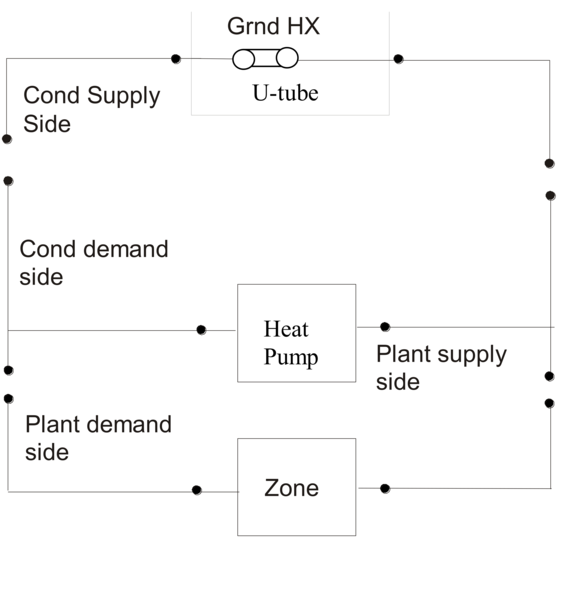
\includegraphics[width=0.9\textwidth, height=0.9\textheight, keepaspectratio=true]{media/image202.png}
\caption{Schematic of EnergyPlus Ground Loop Heat Exchanger \protect \label{fig:schematic-of-energyplus-ground-loop-heat}}
\end{figure}

Definitions for the input fields are provided below.

\subsubsection{Inputs}\label{inputs-10-002}

\paragraph{Field: Name}\label{field-name-9-003}

This alpha field contains the identifying name for the ground heat exchanger (GHE).

\paragraph{Field: Inlet Node Name}\label{field-inlet-node-name-000}

This alpha field contains the ground heat exchanger inlet node name.

\paragraph{Field: Outlet Node Name}\label{field-outlet-node-name-001}

This alpha field contains the ground heat exchanger outlet node name.

\paragraph{Field: Design Flow Rate}\label{field-design-flow-rate-000}

This numeric field contains the GHE design flow rate in cubic meters per second \{m\(^{3}\)/s\}. The flow rate specified is the total flow rate for the entire borehole field. Flow will be assumed to be evenly distributed across all boreholes.

\paragraph{Field: Type of Undisturbed Ground Temperature Object}\label{field-type-of-undisturbed-ground-temperature-object}

The type of undisturbed ground temperature object used to determine ground temperature for the farfield boundary conditions.

\paragraph{Field: Name of Undisturbed Ground Temperature Object}\label{field-name-of-undisturbed-ground-temperature-object}

The name of the undisturbed ground temperature object used to determine ground temperature for the farfield boundary conditions.

\paragraph{Field: Ground Thermal Conductivity}\label{field-ground-thermal-conductivity}

This numeric field contains the thermal conductivity of the ground in W/m-K.

\paragraph{FieldSet: Ground Thermal Heat Capacity}\label{fieldset-ground-thermal-heat-capacity}

This numeric field contains the thermal heat capacity of the ground in J/m\(^{3}\)-K.

\paragraph{Field: GHE:ResponseFactors object name}

The unique name of the \hyperref[groundheatexchangerresponsefactors]{GroundHeatExchanger:ResponseFactors} object used to define the third-party response factors. If present, the GHE:Vertical:Array and GHE:Vertical:Single objects defined will be ignored.

\paragraph{Field: g-Function Calculation Method}

If the GHE:ResponseFactors object is not provided, this input will be relevant to the calculation method used to generate the g-function values. There are two options for this input: ``UHFcalc" or ``UBHWTcalc". The default is UHFcalc, where a g-function is computed with the uniform heat flux boundary condition. The UBHWTcalc option computes the g-function with a uniform borehole wall temperature boundary condition. The g-function computed with a uniform borehole wall temperature boundary condition is expected to be a better approximation of the borehole physics and is also expected to be faster to compute.

\paragraph{Field: GHE:Vertical:Array object name}

The unique name of the \hyperref[groundheatexchangerverticalarray]{GroundHeatExchanger:Vertical:Array} object used to define a rectangular borehole field. If present, the GHE:Vertical:Single objects will be ignored.

\paragraph{Field: GHE:Vertical:Single names}

The unique names of all single, vertical GLHE objects which are used to define and arbitrarily shaped GHE array. This field is extensible.

The following is are example inputs corresponding to the input variations allowed which were described previously. The first example uses the \hyperref[groundheatexchangerverticalarray]{GroundHeatExchanger:Vertical:Array} object. The g-functions will be generated automatically by EnergyPlus and cached for later use.

\begin{lstlisting}
  GroundHeatExchanger:System,
    Vertical GHE 1x4 Std,  !- Name
    GLHE Inlet,         !- Inlet Node Name
    GLHE Outlet,        !- Outlet Node Name
    0.00100944,         !- Design Flow Rate {m3/s}
    Site:GroundTemperature:Undisturbed:KusudaAchenbach,  !- Undisturbed Ground Temperature Model Type
    KATemps,            !- Undisturbed Ground Temperature Model Name
    2.5,                !- Ground Thermal Conductivity {W/m-K}
    2.5E+06,            !- Ground Thermal Heat Capacity {J/m3-K}
    ,                   !- Response Factors Object Name
    UBHWTcalc,          !- g-Function Calculation Method
    GHE-Array;          !- GHE:Vertical:Array Object Name

  GroundHeatExchanger:Vertical:Properties,
    GHE-1 Props,        !- Name
    1,                  !- Depth of Top of Borehole {m}
    100,                !- Borehole Length {m}
    0.114,              !- Borehole Diameter {m}
    0.7443,             !- Grout Thermal Conductivity {W/m-K}
    3.90E+06,           !- Grout Thermal Heat Capacity {J/m3-K}
    0.3895,             !- Pipe Thermal Conductivity {W/m-K}
    1.77E+06,           !- Pipe Thermal Heat Capacity {J/m3-K}
    0.03341,            !- Pipe Outer Diameter {m}
    0.002984,           !- Pipe Thickness {m}
    0.04913;            !- U-Tube Distance {m}

  GroundHeatExchanger:Vertical:Array,
    GHE-Array,          !- Name
    GHE-1 Props,        !- GHE Properties
    2,                  !- Number of Boreholes in X Direction
    2,                  !- Number of Boreholes in Y Direction
    5;                  !- Borehole Spacing {m}
\end{lstlisting}

The second example uses the \hyperref[groundheatexchangerverticalsingle]{GroundHeatExchanger:Vertical:Single} object. The g-functions will be generated automatically by EnergyPlus and cached for later use.

\begin{lstlisting}
  GroundHeatExchanger:System,
    Vertical GHE 1x4 Std,  !- Name
    GLHE Inlet,         !- Inlet Node Name
    GLHE Outlet,        !- Outlet Node Name
    0.00100944,         !- Design Flow Rate {m3/s}
    Site:GroundTemperature:Undisturbed:KusudaAchenbach,  !- Undisturbed Ground Temperature Model Type
    KATemps,            !- Undisturbed Ground Temperature Model Name
    2.5,                !- Ground Thermal Conductivity {W/m-K}
    2.5E+06,            !- Ground Thermal Heat Capacity {J/m3-K}
    ,                   !- Response Factors Object Name
    UBHWTcalc,          !- g-Function Calculation Method
    ,                   !- GHE Array Object Name
    GHE-1,              !- GHE Borehole Definition 1
    GHE-2,              !- GHE Borehole Definition 2
    GHE-3,              !- GHE Borehole Definition 3
    GHE-4;              !- GHE Borehole Definition 4

  GroundHeatExchanger:Vertical:Properties,
    GHE-1 Props,        !- Name
    1,                  !- Depth of Top of Borehole {m}
    100,                !- Borehole Length {m}
    0.114,              !- Borehole Diameter {m}
    0.7443,             !- Grout Thermal Conductivity {W/m-K}
    3.90E+06,           !- Grout Thermal Heat Capacity {J/m3-K}
    0.3895,             !- Pipe Thermal Conductivity {W/m-K}
    1.77E+06,           !- Pipe Thermal Heat Capacity {J/m3-K}
    0.03341,            !- Pipe Outer Diameter {m}
    0.002984,           !- Pipe Thickness {m}
    0.04913;            !- U-Tube Distance {m}

  GroundHeatExchanger:Vertical:Single,
    GHE-1,              !- Name
    GHE-1 Props,        !- GHE Properties
    0,                  !- X Location {m}
    0;                  !- Y Location {m}

  GroundHeatExchanger:Vertical:Single,
    GHE-2,              !- Name
    GHE-1 Props,        !- GHE Properties
    5,                  !- X Location {m}
    0;                  !- Y Location {m}

  GroundHeatExchanger:Vertical:Single,
    GHE-3,              !- Name
    GHE-1 Props,        !- GHE Properties
    0,                  !- X Location {m}
    5;                  !- Y Location {m}

  GroundHeatExchanger:Vertical:Single,
    GHE-4,              !- Name
    GHE-1 Props,        !- GHE Properties
    5,                  !- X Location {m}
    5;                  !- Y Location {m}
\end{lstlisting}

The final example uses the ResponseFactors object to provide third-party g-functions.

\begin{lstlisting}
  GroundHeatExchanger:System,
    Vertical GHE 1x4 Std,  !- Name
    GLHE Inlet,         !- Inlet Node Name
    GLHE Outlet,        !- Outlet Node Name
    0.00100944,         !- Design Flow Rate {m3/s}
    Site:GroundTemperature:Undisturbed:KusudaAchenbach,  !- Undisturbed Ground Temperature Model Type
    KATemps,            !- Undisturbed Ground Temperature Model Name
    2.5,                !- Ground Thermal Conductivity {W/m-K}
    2.5E+06,            !- Ground Thermal Heat Capacity {J/m3-K}
    GHE-1 g-functions;  !- Response Factors Object Name

  GroundHeatExchanger:Vertical:Properties,
    GHE-1 Props,        !- Name
    1,                  !- Depth of Top of Borehole {m}
    100,                !- Borehole Length {m}
    0.114,              !- Borehole Diameter {m}
    0.7443,             !- Grout Thermal Conductivity {W/m-K}
    3.90E+06,           !- Grout Thermal Heat Capacity {J/m3-K}
    0.3895,             !- Pipe Thermal Conductivity {W/m-K}
    1.77E+06,           !- Pipe Thermal Heat Capacity {J/m3-K}
    0.03341,            !- Pipe Outer Diameter {m}
    0.002984,           !- Pipe Thickness {m}
    0.04913;            !- U-Tube Distance {m}

  GroundHeatExchanger:ResponseFactors,
    GHE-1 g-functions,       !- Name
    GHE-1 Props,             !- GHE Properties
    4,                       !- Number of Boreholes
    0.00043,                 !- G-Function Reference Ratio {dimensionless}
    -15.585075,              !- G-Function Ln(T/Ts) Value 1
    -2.672011,               !- G-Function G Value 1
    -15.440481,              !- G-Function Ln(T/Ts) Value 2
    -2.575897,               !- G-Function G Value 2
    -15.295888,              !- G-Function Ln(T/Ts) Value 3
    -2.476279,               !- G-Function G Value 3
    -15.151295,              !- G-Function Ln(T/Ts) Value 4
    -2.372609,               !- G-Function G Value 4
    ...,
    12.365217,               !- G-Function G Value 70
    1.112000,                !- G-Function Ln(T/Ts) Value 71
    12.469007,               !- G-Function G Value 71
    1.335000,                !- G-Function Ln(T/Ts) Value 72
    12.547123,               !- G-Function G Value 72
    1.679000;                !- G-Function Ln(T/Ts) Value 73
\end{lstlisting}

\subsubsection{Outputs}\label{outputs-10-000}

\begin{itemize}
\item
  HVAC,Average,Ground Heat Exchanger Average Borehole Temperature {[}C{]}
\item
  HVAC,Average,Ground Heat Exchanger Heat Transfer Rate {[}W{]}
\item
  HVAC,Average,Ground Heat Exchanger Inlet Temperature {[}C{]}
\item
  HVAC,Average,Ground Heat Exchanger Outlet Temperature {[}C{]}
\item
  HVAC,Average,Ground Heat Exchanger Mass Flow Rate {[}kg/s{]}
\item
  HVAC,Average,Ground Heat Exchanger Average Fluid Temperature {[}C{]}
\item
  HVAC,Average,Ground Heat Exchanger Farfield Ground Temperature {[}C{]}
\end{itemize}

\paragraph{Ground Heat Exchanger Average Borehole Temperature {[}C{]}}\label{ground-heat-exchanger-average-borehole-temperature-c}

This is the model result for the average temperature of the borehole heat exchanger.

\paragraph{Ground Heat Exchanger Heat Transfer Rate {[}W{]}}\label{ground-heat-exchanger-heat-transfer-rate-w}

This is the rate of heat transfer between the working fluid and the ground heat exchanger, in Watts.

\paragraph{Ground Heat Exchanger Inlet Temperature {[}C{]}}\label{ground-heat-exchanger-inlet-temperature-c}

This is the temperature of the working fluid entering the ground heat exchanger.

\paragraph{Ground Heat Exchanger Outlet Temperature {[}C{]}}\label{ground-heat-exchanger-outlet-temperature-c}

This is the temperature of the working fluid leaving the ground heat exchanger.

\paragraph{Ground Heat Exchanger Mass Flow Rate {[}kg/s{]}}\label{ground-heat-exchanger-mass-flow-rate-kgs}

This is the mass flow rate of the working fluid through the heat exchanger.

\paragraph{Ground Heat Exchanger Average Fluid Temperature {[}C{]}}\label{ground-heat-exchanger-average-fluid-temperature-c}

This is the average temperature of the working fluid inside the heat exchanger.

\paragraph{Ground Heat Exchanger Farfield Ground Temperature}

This is the farfield temperature used by the object which is provided by the undisturbed ground temperature object. The temperature is the average of the 5 evenly spaced points between the top of the borehole and the bottom of the borehole.

\subsection{GroundHeatExchanger:Vertical:Properties}\label{groundheatexchangerverticalproperties}

This object defines several borehole parameters.

\subsubsection{Inputs}

\paragraph{Field: Name}

This alpha field indicates the unique name of the object.

\paragraph{Field: Depth of Top of Borehole}

This numeric field indicates the depth of the top of the borehole below the ground surface, in meters. The depth measured from the ground surface downward is positive.

\paragraph{Field: Borehole Length}

This numeric field indicates the active length of the borehole, referenced from the starting location (potentially below the ground surface), to the end of the borehole, in meters.

\paragraph{Field: Borehole Diameter}

This numeric field indicates the diameter of the borehole, in meters.

\paragraph{Field: Grout Thermal Conductivity}\label{field-grout-thermal-conductivity}

This numeric field contains the thermal conductivity of the filler material in W/m-K.

\paragraph{Field: Grout Thermal Heat Capacity}

This numeric field contains the thermal heat capacity of the grout in J/m\(^{3}\)-K.

\paragraph{Field: Pipe Thermal Conductivity}\label{field-pipe-thermal-conductivity-000}

This numeric field contains the thermal conductivity of the pipe in W/m-K.

\paragraph{Field: Pipe Thermal Heat Capacity}

This numeric field contains the thermal heat capacity of the pipe in J/m\(^{3}\)-K.

\paragraph{Field: Pipe Outer Diameter}\label{field-pipe-out-diameter}

This numeric field contains the outer diameter of the U-tube (pipe) in meters \{m\}.

\paragraph{Field: Pipe Thickness}\label{field-pipe-thickness-000}

This numeric field contains the outer diameter of the U-tube (pipe) in meters.

\paragraph{Field: U-Tube Distance}\label{field-u-tube-distance}

This numeric field contains the distance between the two legs of the U-tube in meters \{m\}. Distance is measured from the u-tube pipe center.

An example object is shown below.

\begin{lstlisting}
  GroundHeatExchanger:Vertical:Properties,
    GHE-1 Props,        !- Name
    1,                  !- Depth of Top of Borehole {m}
    100,                !- Borehole Length {m}
    0.114,              !- Borehole Diameter {m}
    0.7443,             !- Grout Thermal Conductivity {W/m-K}
    3.90E+06,           !- Grout Thermal Heat Capacity {J/m3-K}
    0.3895,             !- Pipe Thermal Conductivity {W/m-K}
    1.77E+06,           !- Pipe Thermal Heat Capacity {J/m3-K}
    0.03341,            !- Pipe Outer Diameter {m}
    0.002984,           !- Pipe Thickness {m}
    0.04913;            !- U-Tube Distance {m}
\end{lstlisting}

\subsection{GroundHeatExchanger:Vertical:Array}\label{groundheatexchangerverticalarray}

This object defines the borehole locations for a rectangular array of boreholes.

\paragraph{Field: Name}

This alpha field indicates the unique name of the object.

\paragraph{Field: Properties}

This alpha field indicates the name of the \hyperref[groundheatexchangerverticalproperties]{GroundHeatExchanger:Vertical:Properties} object referenced by the boreholes in the array.

\paragraph{Field: Number of Boreholes in the X-Direction}

This numeric field indicates the number of boreholes in one axis of the rectangular borehole field.

\paragraph{Field: Number of Boreholes in the Y-Direction}

This numeric field indicates the number of boreholes in the other axis of the rectangular borehole field.

\paragraph{Field: Borehole Spacing}

This numeric field indicates the center-to-center borehole spacing, in meters, which is applied to the rectangular borehole field.

An example object is shown below.

\begin{lstlisting}
  GroundHeatExchanger:Vertical:Array,
    GHE-Array,          !- Name
    GHE-1 Props,        !- GHE Properties
    2,                  !- Number of Boreholes in X Direction
    2,                  !- Number of Boreholes in Y Direction
    5;                  !- Borehole Spacing {m}
\end{lstlisting}

\subsection{GroundHeatExchanger:Vertical:Single}\label{groundheatexchangerverticalsingle}

This object defines a single borehole heat exchanger.

\subsubsection{Inputs}

\paragraph{Field: Name}

This alpha field indicates the unique name of the object.

\paragraph{Field: Properties}

This alpha field indicates the name of the \hyperref[groundheatexchangerverticalproperties]{GroundHeatExchanger:Vertical:Properties} object referenced by the borehole.

\paragraph{Field: X-Location}

This numeric field indicates the x-location of this borehole.

\paragraph{Field: Y-Location}

This numeric field indicates the y-location of this borehole.

\begin{lstlisting}
  GroundHeatExchanger:Vertical:Single,
    GHE-1,              !- Name
    GHE-1 Props,        !- GHE Properties
    0,                  !- X Location {m}
    0;                  !- Y Location {m}
\end{lstlisting}

\subsection{GroundHeatExchanger:ResponseFactors}\label{groundheatexchangerresponsefactors}

This object is used to provide third-party g-functions which are generated by other tools.

\subsubsection{Inputs}

\paragraph{Field: Name}

This alpha field indicates the unique name of the object.

\paragraph{Field: Properties}

This alpha field indicates the name of the \hyperref[groundheatexchangerverticalproperties]{GroundHeatExchanger:Vertical:Properties} object referenced g-function response factors.

\paragraph{Field: G-Function Reference Ratio}\label{field-g-function-reference-ratio}

The G-Functions may be formulated slightly differently based on the program which generated them. The original g-functions as defined by Eskilson are based on an borehole radius to active length ratio of 0.0005. If the physical ratio is different from this, a correction must be applied. EnergyPlus will apply the correction, based on the reference ratio entered in this field. Therefore, therefore two possible input configurations.

\begin{itemize}
\item
  If the g-functions have not had a correction applied, then the g-functions are still based on a reference of 0.0005, so use a value of 0.0005 in this field. EnergyPlus will adjust the g-functions internally to create the properly referenced g-function.
\item
  If the correction has already been applied, then the input g-functions are based on a reference to the actual (physical) radius/length ratio, so enter the physical radius/length in this field. Entering the actual value will nullify any internal corrections, which will avoid re-basing the g-function set.
\end{itemize}

The software GLHEPro has been making this ``pre-correction'' to the data sets since version 3.1 of that software, so this input field should match the actual (physical) radius/length ratio.

\paragraph{Field: g-function Ln(t/ts) Value \textless{}x\textgreater{}}\label{field-g-function-lntts-value-x}

This numeric field contains the natural log of time/steady state time: \emph{ln(t/t\(_{s}\))}.

\paragraph{Field: g-function `g' Value \textless{}x\textgreater{}}\label{field-g-function-g-value-x}

This numeric field contains the g-function value of the corresponding LNTTS.

This object is extensible, so additional pairs of these last two fields can be added to the end of this object.

An example object is shown below.

\begin{lstlisting}
  GroundHeatExchanger:ResponseFactors,
    GHE-1 g-functions,       !- Name
    GHE-1 Props,             !- GHE Properties
    4,                       !- Number of Boreholes
    0.0005,                  !- G-Function Reference Ratio {dimensionless}
    -15.585075,              !- G-Function Ln(T/Ts) Value 1
    -2.672011,               !- G-Function G Value 1
    -15.440481,              !- G-Function Ln(T/Ts) Value 2
    -2.575897,               !- G-Function G Value 2
    -15.295888,              !- G-Function Ln(T/Ts) Value 3
    -2.476279,               !- G-Function G Value 3
    -15.151295,              !- G-Function Ln(T/Ts) Value 4
    -2.372609,               !- G-Function G Value 4
    ...,
    12.365217,               !- G-Function G Value 70
    1.112000,                !- G-Function Ln(T/Ts) Value 71
    12.469007,               !- G-Function G Value 71
    1.335000,                !- G-Function Ln(T/Ts) Value 72
    12.547123,               !- G-Function G Value 72
    1.679000;                !- G-Function Ln(T/Ts) Value 73
\end{lstlisting}

\subsection{GroundHeatExchanger:Slinky}\label{groundheatexchangerslinky}

The GroundHeatExchanger:Slinky use the g-functions to calculate the GHX temperature response, similar to the GroundHeatExchanger:Vertical model, however for this model g-functions are automatically calculated by EnergyPlus without the need of external software or data.

Horizontal slinky-loop ground heat exchangers (GHXs) consist of coiled tubing, with the individual rings spread out along the direction of the trench either horizontally or vertically, as shown in \protect\hyperlink{SlinkyIOFig1}{Figure}. A schematic of a slinky GHX can be seen in \protect\hyperlink{SlinkyIOFig2}{Figure}. Compared to conventional straight tube horizontal GHXs, slinky loops have a higher tube density; hence, with the same cooling/heating loads, slinky-loop GHXs require less land area and excavation work than straight tube HGHXs.

\begin{figure}[htbp]
\centering
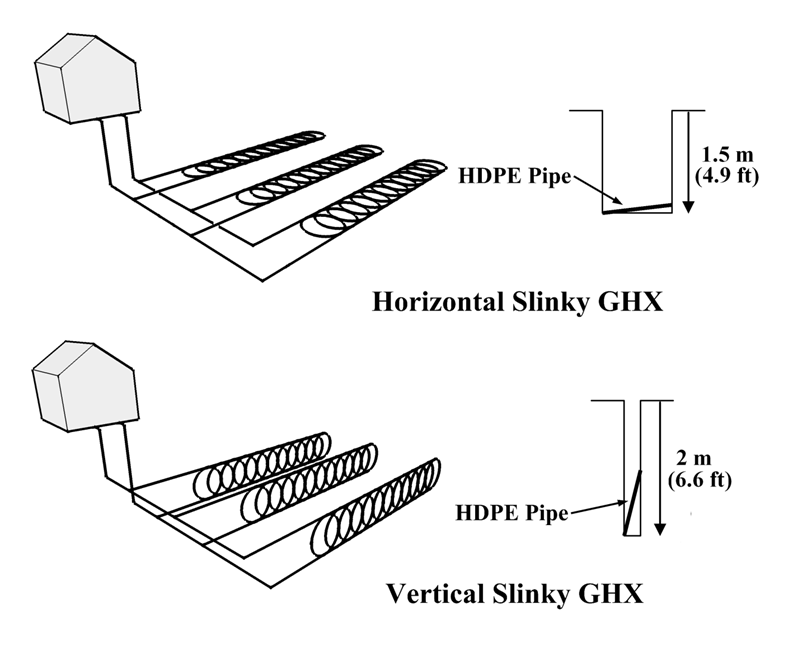
\includegraphics{media/image901.png}
\caption{slinky heat exchanger}
\end{figure}

Figure: Slinky Ground Heat Exchanger Configurations.

\begin{figure}[htbp]
\centering
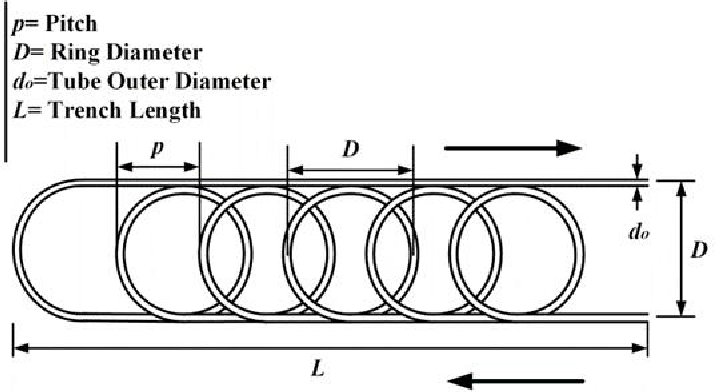
\includegraphics{media/image902.png}
\caption{slinky heat exchanger}
\end{figure}

Figure: Schematic of Slinky HX.

An example GroundHeatExchanger:Slinky object is shown below.

\begin{lstlisting}

GroundHeatExchanger:Slinky,
  Slinky GHX,       !- Name
  GHE Inlet Node,   !- Inlet Node
  GHE Outlet Node,  !- Outlet Node
  0.0033,           !- Design Flow Rate [m3/s]
  1.2,              !- Soil Thermal Conductivity [W/m-K]
  3200,             !- Soil Density [kg/m3]
  850,              !- Soil Specific Heat [J/kg-K]
  1.8,              !- Pipe Thermal Conductivity [W/m-K]
  920,              !- Pipe Density [kg/m3]
  2200,             !- Pipe Specific Heat [J/kg-K]
  0.02667,          !- Pipe Outside Diameter [m]
  0.002413,         !- Pipe Wall Thickness [m]
  Vertical,         !- Heat Exchanger Configuration (Vertical, Horizontal)
  1,                !- Coil Diameter [m]
  0.2,              !- Coil Pitch [m]
  2.5,              !- Trench Depth [m]
  40,               !- Trench Length [m]
  15,               !- Number of Parallel Trenches
  2,                !- Trench Spacing [m]
  Site:GroundTemperature:Undisturbed:KusudaAchenbach, !- Type of Undisturbed Ground Temperature Object
  KATemps,          !- Name of Undisturbed Ground Temperature Object
  10;               !- Maximum length of simulation [years]
\end{lstlisting}

\subsubsection{Inputs}\label{inputs-11-002}

\paragraph{Field: Name}\label{field-name-10-002}

Alpha field used as identifying field for heat exchanger

\paragraph{Field: Inlet Node}\label{field-inlet-node}

This alpha field is the name of the inlet node of the component on a plant loop.

\paragraph{Field: Outlet Node}\label{field-outlet-node}

This alpha field is the name of the outlet node of the component on a plant loop.

\paragraph{Field: Design Flow Rate}\label{field-design-flow-rate-1-000}

This numeric field is the design flow rate in m3/s for the heat exchanger. The plant loop will attempt to meet this request based on loop and flow conditions.

\paragraph{Field: Soil Thermal Conductivity}\label{field-soil-thermal-conductivity}

This numeric field is the thermal conductivity of the soil, in W/m-K.

\paragraph{Field: Soil Density}\label{field-soil-density}

This numeric field is the density of the soil, in kg/m3.

\paragraph{Field: Soil Specific Heat}\label{field-soil-specific-heat}

This numeric field is the specific heat of the soil, in J/kg-K.

\paragraph{Field: Pipe Thermal Conductivity}\label{field-pipe-thermal-conductivity-1}

This numeric field is the thermal conductivity of the heat exchanger pipe.

\paragraph{Field: Pipe Density}\label{field-pipe-density}

This numeric field is the density of the heat exchanger pipe, in kg/m3.

\paragraph{Field: Pipe Specific Heat}\label{field-pipe-specific-heat}

This numeric field is the specific heat of the heat exchanger pipe, in J/kg-K.

\paragraph{Field: Pipe Outside Diameter}\label{field-pipe-outside-diameter}

This numeric field is the outside pipe diameter, in meters.

\paragraph{Field: Pipe Wall Thickness}\label{field-pipe-wall-thickness}

This numeric field is the pipe wall thickness, in meters.

\paragraph{Field: Heat Exchanger Configuration}\label{field-heat-exchanger-configuration}

This alpha field is heat exchanger configuration, either Vertical or Horizontal.

\paragraph{Field: Coil Diameter}\label{field-coil-diameter}

This numeric is the diameter of the slinky coil, in meters.

\paragraph{Field: Coil Pitch}\label{field-coil-pitch}

This numeric field is the center-to-center distance between heat exchanger coils, in meters.

\paragraph{Field: Trench Depth}\label{field-trench-depth}

This numeric field is the distance from the bottom of the trench to the ground surface, in meters.

\paragraph{Field: Trench Length}\label{field-trench-length}

This numeric field is the length of the heat exchanger trench, in meters. This assumes the heat exchanger runs the full length of the trench.

\paragraph{Field: Number of Parallel Trenches}\label{field-number-of-parallel-trenches}

This numeric field is the number of parallel trenches. Design flow rate will be equally divided among all parallel trenches.

\paragraph{Field: Trench Spacing}\label{field-trench-spacing}

This numeric field is the center-to-center distance in between parallel trenches, in meters.

\paragraph{Field: Type of Undisturbed Ground Temperature Object}

The type of undisturbed ground temperature object used to determine ground temperature for the farfield boundary conditions.

\paragraph{Field: Name of Undisturbed Ground Temperature Object}

The name of the undisturbed ground temperature object used to determine ground temperature for the farfield boundary conditions.

\paragraph{Field: Maximum Length of Simulation}\label{field-maximum-length-of-simulation-1}

This numeric field contains the maximum number of years of simulation to be carried out.

\subsubsection{Outputs}\label{outputs-11-000}

The following output variables are available.

\begin{itemize}
\item
  HVAC,Average,Ground Heat Exchanger Average Borehole Temperature {[}C{]}
\item
  HVAC,Average,Ground Heat Exchanger Heat Transfer Rate {[}W{]}
\item
  HVAC,Average,Ground Heat Exchanger Inlet Temperature {[}C{]}
\item
  HVAC,Average,Ground Heat Exchanger Outlet Temperature {[}C{]}
\item
  HVAC,Average,Ground Heat Exchanger Mass Flow Rate {[}kg/s{]}
\item
  HVAC,Average,Ground Heat Exchanger Average Fluid Temperature {[}C{]}
\end{itemize}

\paragraph{Ground Heat Exchanger Average Borehole Temperature {[}C{]}}\label{ground-heat-exchanger-average-borehole-temperature-c-1}

This is the model result for the average temperature of the borehole heat exchanger.

\paragraph{Ground Heat Exchanger Heat Transfer Rate {[}W{]}}\label{ground-heat-exchanger-heat-transfer-rate-w-1}

This is the rate of heat transfer between the working fluid and the ground heat exchanger, in Watts.

\paragraph{Ground Heat Exchanger Inlet Temperature {[}C{]}}\label{ground-heat-exchanger-inlet-temperature-c-1}

This is the temperature of the working fluid entering the ground heat exchanger.

\paragraph{Ground Heat Exchanger Outlet Temperature {[}C{]}}\label{ground-heat-exchanger-outlet-temperature-c-1}

This is the temperature of the working fluid leaving the ground heat exchanger.

\paragraph{Ground Heat Exchanger Mass Flow Rate {[}kg/s{]}}\label{ground-heat-exchanger-mass-flow-rate-kgs-1}

This is the mass flow rate of the working fluid through the heat exchanger.

\paragraph{Ground Heat Exchanger Average Fluid Temperature {[}C{]}}\label{ground-heat-exchanger-average-fluid-temperature-c-1}

This is the average temperature of the working fluid inside the heat exchanger.

\subsection{GroundHeatExchanger:Pond}\label{groundheatexchangerpond}

The pond heat exchanger model represents a shallow pond with submerged hydronic tubes through which the heat transfer fluid is circulated. The model represents a `shallow' pond in that no attempt is made to model any stratification effects that may~ be present in deeper ponds.

This type of heat exchanger is intended to be connected to the supply side of a condenser loop, and can be used with any type of plant loop. The pond may be specified as the only heat exchanger on the condenser loop (as shown in Figure~\ref{fig:example-of-pond-ground-heat-exchanger-as-only}) or it may be connected in parallel with other condenser loop heat exchangers (such as cooling towers, ground surface heat exchangers) as shown in the second figure below.

\begin{figure}[hbtp] % fig 84
\centering
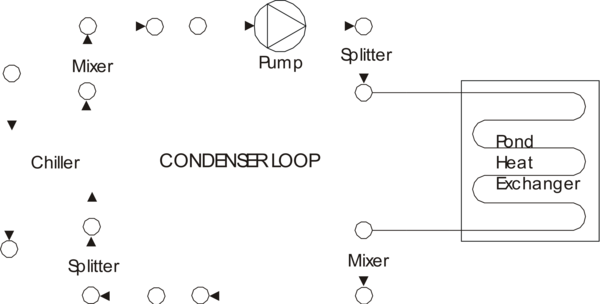
\includegraphics[width=0.9\textwidth, height=0.9\textheight, keepaspectratio=true]{media/image203.png}
\caption{Example of Pond Ground Heat Exchanger as only heat exchanger on condenser loop \protect \label{fig:example-of-pond-ground-heat-exchanger-as-only}}
\end{figure}

\begin{figure}[hbtp] % fig 85
\centering
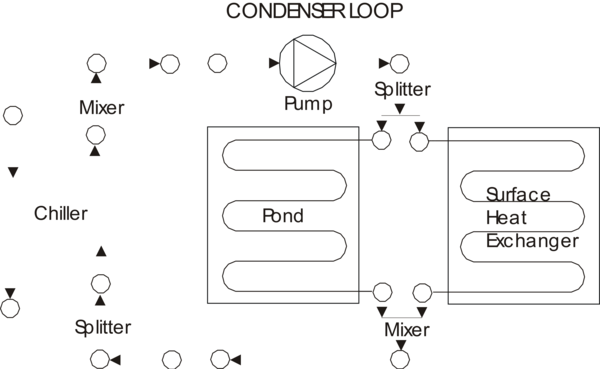
\includegraphics[width=0.9\textwidth, height=0.9\textheight, keepaspectratio=true]{media/image204.png}
\caption{Pond Ground Heat Exchanger with other heat exchangers on condenser loop \protect \label{fig:pond-ground-heat-exchanger-with-other-heat}}
\end{figure}

\subsubsection{Inputs}\label{inputs-12-002}

\paragraph{Field: Name}\label{field-name-11-002}

This alpha field contains the identifying name for the outside pond heat exchanger.

\paragraph{Field: Fluid Inlet Node Name}\label{field-fluid-inlet-node-name}

This alpha field contains the fluid inlet node name.

\paragraph{Field: Fluid Outlet Node Name}\label{field-fluid-outlet-node-name}

This alpha field contains the fluid outlet node name.

\paragraph{Field: Pond Depth}\label{field-pond-depth}

This numeric field contains the pond depth \{m\}.

\paragraph{Field: Pond Area}\label{field-pond-area}

This numeric field contains the pond area m\(^{2}\).

\paragraph{Field: Hydronic Tubing Inside Diameter}\label{field-hydronic-tubing-inside-diameter}

This numeric field contains the hydronic tubing inside diameter \{m\}.

\paragraph{Field: Hydronic Tubing Outside Diameter}\label{field-hydronic-tubing-outside-diameter}

This numeric field contains the hydronic tubing outside diameter \{m\}.

\paragraph{Field: Hydronic Tubing Thermal Conductivity}\label{field-hydronic-tubing-thermal-conductivity}

This numeric field contains the hydronic tubing thermal conductivity in W/mK.

\paragraph{Field: Ground Thermal Conductivity}\label{field-ground-thermal-conductivity-1}

This numeric field contains the ground thermal conductivity in W/m\(^{2}\)K.

\paragraph{Field: Number of Tubing Circuits}\label{field-number-of-tubing-circuits}

This numeric field contains the number of hydronic tubing circuits, total in parallel in this pond..

\paragraph{Field: Length of Each Tubing Circuit}\label{field-length-of-each-tubing-circuit}

This numeric field contains length \{m\} of each hydronic tubing circuit.

An example of the IDF is shown below.

\begin{lstlisting}

  GroundHeatExchanger:Pond,
      Pond 1,                  !- Name
      Condenser Tower 1 Inlet Node,  !- Fluid Inlet Node Name
      Condenser Tower 1 Outlet Node,  !- Fluid Outlet Node Name
      2.0,                     !- Pond Depth {m}
      1000.0,                  !- Pond Area {m2}
      0.02,                    !- Hydronic Tubing Inside Diameter {m}
      0.025,                   !- Hydronic Tubing Outside Diameter {m}
      0.4,                     !- Hydronic Tubing Thermal Conductivity {W/m-K}
      1.0,                     !- Ground Thermal Conductivity {W/m2-K}
      10,                      !- Number of Tubing Circuits
      50.0;                    !- Length of Each Tubing Circuit {m}
\end{lstlisting}

\subsubsection{Outputs}\label{outputs-12-000}

\begin{itemize}
\item
  HVAC,Average,Pond Heat Exchanger Heat Transfer Rate {[}W{]}
\item
  HVAC,Sum,Pond Heat Exchanger Heat Transfer Energy {[}J{]}
\item
  HVAC,Average,Pond Heat Exchanger Mass Flow Rate {[}kg/s{]}
\item
  HVAC,Average,Pond Heat Exchanger Inlet Temperature {[}C{]}
\item
  HVAC,Average,Pond Heat Exchanger Outlet Temperature {[}C{]}
\item
  HVAC,Average,Pond Heat Exchanger Bulk Temperature {[}C{]}
\end{itemize}

\paragraph{Pond Heat Exchanger Heat Transfer Rate {[}W{]}}\label{pond-heat-exchanger-heat-transfer-rate-w}

\paragraph{Pond Heat Exchanger Heat Transfer Energy {[}J{]}}\label{pond-heat-exchanger-heat-transfer-energy-j}

These outputs are the pond ground heat exchanger heat transfer rate and total energy exchange for the timestep.

\paragraph{Pond Heat Exchanger Mass Flow Rate {[}kg/s{]}}\label{pond-heat-exchanger-mass-flow-rate-kgs}

\paragraph{Pond Heat Exchanger Inlet Temperature {[}C{]}}\label{pond-heat-exchanger-inlet-temperature-c}

\paragraph{Pond Heat Exchanger Outlet Temperature {[}C{]}}\label{pond-heat-exchanger-outlet-temperature-c}

These outputs are the pond fluid inlet and outlet temperatures and mass flow rate.

\paragraph{Pond Heat Exchanger Bulk Temperature {[}C{]}}\label{pond-heat-exchanger-bulk-temperature-c}

This output is the pond bulk temperature.

\subsection{GroundHeatExchanger:Surface}\label{groundheatexchangersurface}

The surface heat exchanger model is to simulate hydronic surface ground heat exchangers. This includes pavement surfaces with embedded pipes for snow-melting or heat rejection from hybrid ground source heat pump systems.

The heat exchanger may be ground coupled or not. In the latter case the bottom surface is exposed to the wind but not solar gains. This type of heat exchanger is intended to be connected to the supply side of a condenser loop, and can be used with any type of plant loop. The surface heat exchanger may be specified as the only heat exchanger on the condenser loop (as shown in the first figure below) or it may be connected in parallel with other condenser loop heat exchangers (such as cooling towers, ground surface heat exchangers) as shown in the second figure below.

\begin{figure}[hbtp] % fig 86
\centering
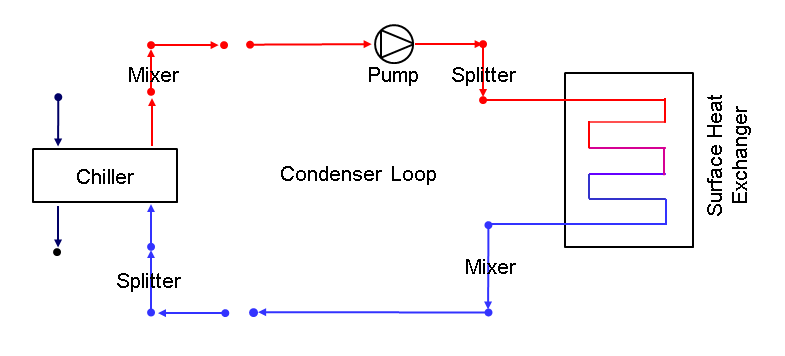
\includegraphics[width=0.9\textwidth, height=0.9\textheight, keepaspectratio=true]{media/image205.png}
\caption{Example of Surface Ground Heat Exchanger as only heat exchanger on condenser loop \protect \label{fig:example-of-surface-ground-heat-exchanger}}
\end{figure}

\begin{figure}[hbtp] % fig 87
\centering
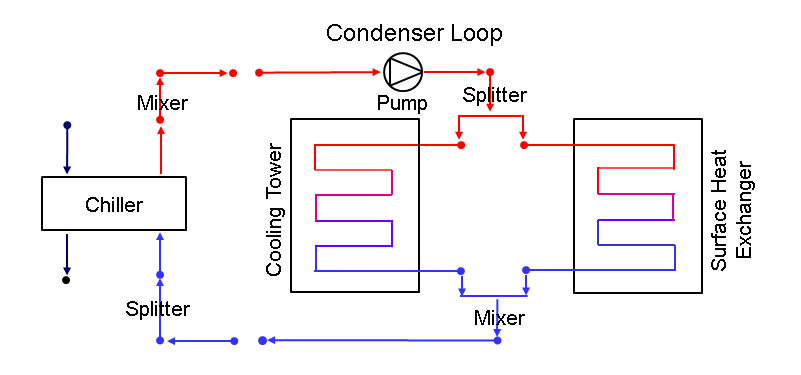
\includegraphics[width=0.9\textwidth, height=0.9\textheight, keepaspectratio=true]{media/image206.png}
\caption{Surface Ground Heat Exchanger with other heat exchangers on condenser loop \protect \label{fig:surface-ground-heat-exchanger-with-other-heat}}
\end{figure}

\subsubsection{Inputs}\label{inputs-13-002}

\paragraph{Field: Name}\label{field-name-12-001}

This alpha field contains the identifying name for the outside panel heat exchanger.

\paragraph{Field: Construction Name}\label{field-construction-name-000}

This alpha field contains the construction name. It must contain a valid ``Construction'' name that is usual for Surfaces. (Ref: Group -- Surface Construction Elements).

\paragraph{Field: Fluid Inlet Node Name}\label{field-fluid-inlet-node-name-1}

This alpha field contains the fluid inlet node name.

\paragraph{Field: Fluid Outlet Node Name}\label{field-fluid-outlet-node-name-1}

This alpha field contains the fluid outlet node name.

\paragraph{Field: Hydronic Tubing Inside Diameter}\label{field-hydronic-tubing-inside-diameter-1}

This numeric field contains the hydronic tubing inside diameter in m.

\paragraph{Field: Number of Tubing Circuits}\label{field-number-of-tubing-circuits-1}

This numeric field contains the number of hydronic tubing circuits.

\paragraph{Field: Hydronic Tube Spacing}\label{field-hydronic-tube-spacing}

This numeric field contains the hydronic tube spacing in m.

\paragraph{Field: Surface Length}\label{field-surface-length}

This numeric field contains the surface length in m.

\paragraph{Field: Surface Width}\label{field-surface-width}

This numeric field contains the surface width in m.

\paragraph{Field: Lower Surface Environment}\label{field-lower-surface-environment}

This alpha field expresses the lower surface exposure: Exposed or Ground.

An example of this statement in an IDF is shown below:

\begin{lstlisting}

  GroundHeatExchanger:Surface,
      SURFACE 1,               !- Name
      Outside Surface Construction,  !- Construction Name
      Condenser Tower 1 Inlet Node,  !- Fluid Inlet Node Name
      Condenser Tower 1 Outlet Node,  !- Fluid Outlet Node Name
      0.02,                    !- Hydronic Tubing Inside Diameter {m}
      10.0,                    !- Number of Tubing Circuits
      0.3,                     !- Hydronic Tube Spacing {m}
      100.0,                   !- Surface Length {m}
      100.0,                   !- Surface Width {m}
      GROUND;                  !- Lower Surface Environment
\end{lstlisting}

\subsubsection{Outputs}\label{outputs-13-000}

\begin{itemize}
\item
  HVAC,Average,Ground Heat Exchanger Heat Transfer Rate {[}W{]}
\item
  HVAC,Average,Ground Heat Exchanger Surface Heat Transfer Rate {[}W{]}
\item
  HVAC,Sum,Ground Heat Exchanger Heat Transfer Energy {[}J{]}
\item
  HVAC,Average,Ground Heat Exchanger Mass Flow Rate {[}kg/s{]}
\item
  HVAC,Average,Ground Heat Exchanger Inlet Temperature {[}C{]}
\item
  HVAC,Average,Ground Heat Exchanger Outlet Temperature {[}C{]}
\item
  HVAC,Average,Ground Heat Exchanger Top Surface Temperature {[}C{]}
\item
  HVAC,Average Ground Heat Exchanger Bottom Surface Temperature {[}C{]}
\item
  HVAC,Average,Ground Heat Exchanger Top Surface Heat Transfer Energy per Area {[}J/m2{]}
\item
  HVAC,Average,Ground Heat Exchanger Bottom Surface Heat Transfer Energy per Area{[}J/m2{]}
\item
  HVAC,Sum,Ground Heat Exchanger Surface Heat Transfer Energy {[}J{]}
\item
  HVAC,Average,Ground Heat Exchanger Source Temperature {[}C{]}
\end{itemize}

\paragraph{Ground Heat Exchanger Heat Transfer Rate {[}W{]}}\label{ground-heat-exchanger-heat-transfer-rate-w-2}

\paragraph{Ground Heat Exchanger Surface Heat Transfer Rate {[}W{]}}\label{ground-heat-exchanger-surface-heat-transfer-rate-w}

\paragraph{Ground Heat Exchanger Heat Transfer Energy {[}J{]}}\label{ground-heat-exchanger-heat-transfer-energy-j}

These outputs are the source heat transfer rate, surface heat transfer rate and the total source energy input for the timestep.

\paragraph{Ground Heat Exchanger Mass Flow Rate {[}kg/s{]}}\label{ground-heat-exchanger-mass-flow-rate-kgs-2}

\paragraph{Ground Heat Exchanger Inlet Temperature {[}C{]}}\label{ground-heat-exchanger-inlet-temperature-c-2}

\paragraph{Ground Heat Exchanger Outlet Temperature {[}C{]}}\label{ground-heat-exchanger-outlet-temperature-c-2}

These outputs are the surface heat exchanger fluid inlet and outlet temperatures and mass flow rate.

\paragraph{Ground Heat Exchanger Top Surface Temperature {[}C{]}}\label{ground-heat-exchanger-top-surface-temperature-c}

\paragraph{Ground Heat Exchanger Bottom Surface Temperature {[}C{]}}\label{ground-heat-exchanger-bottom-surface-temperature-c}

These outputs are the surface heat exchanger top and bottom surface temperatures.

\paragraph{Ground Heat Exchanger Top Surface Heat Transfer Energy per Area~ {[}J/m\(^{2}\){]}}\label{ground-heat-exchanger-top-surface-heat-transfer-energy-per-area-jm2}

\paragraph{Ground Heat Exchanger Bottom Surface Heat Transfer Energy per Area {[}J/m\(^{2}\){]}}\label{ground-heat-exchanger-bottom-surface-heat-transfer-energy-per-area-jm2}

These outputs are the surface heat exchanger top and bottom surface flux.

\paragraph{Ground Heat Exchanger Surface Heat Transfer Energy {[}J{]}}\label{ground-heat-exchanger-surface-heat-transfer-energy-j}

This is the total surface energy exchange for the timestep.

\paragraph{Ground Heat Exchanger Source Temperature {[}C{]}}\label{ground-heat-exchanger-source-temperature-c}

This is the surface heat exchanger source temperature.

\subsection{GroundHeatExchanger:HorizontalTrench}\label{groundheatexchangerhorizontaltrench}

The horizontal trench ground heat exchanger object provides an alternate interface to the detailed PipingSystem:Underground:* objects.~ The same underlying simulation algorithm is utilized, providing a transient numerical simulation of soil with buried pipes and a detailed surface heat balance.~ The input syntax is much smaller and useful for simple applications.~ For full flexibility, use the PipingSystem:Underground:* objects to build a detailed simulation domain and piping circuit.~ For information regarding the simulation algorithms, see the engineering reference document section covering the buried piping system objects.

\textbf{\emph{Field: Name}}

This alpha field is used as an identifying field for the ground heat exchanger.

\textbf{\emph{Field: Inlet Node Name}}

This alpha field is the name of the inlet node of this component on a plant loop, and must match other topology definitions such as branch objects.

\textbf{\emph{Field: Outlet Node Name}}

This alpha field is the name of the outlet node of this component on a plant loop, and must match other topology definitions such as branch objects.

\textbf{\emph{Field: Design Flow Rate {[}m3/s{]}}}

This numeric field is the designed flow rate for this heat exchanger; the plant loop solver will attempt to meet this request based on flow and loop conditions.

\textbf{\emph{Field: Trench Length in Pipe Axial Direction {[}m{]}}}

This numeric field represents the axial length of each pipe trench.~ Each pipe defined for this ground heat exchanger will have the same length.~ If different pipes have different lengths, they must use separate GroundHeatExchanger:HorizontalTrench objects with different lengths.

\textbf{\emph{Field: Number of Trenches}}

This integer field is the number of trenches for this heat exchanger.~ Since each trench has a single pipe, this defines the number of ``pipe segments'' for this overall heat exchanger.~ The total piping length is then calculated as the trench length times the number of trenches.

\textbf{\emph{Field: Horizontal Spacing Between Pipes {[}m{]}}}

This numeric field represents the horizontal spacing (pipe centroid to pipe centroid) between pipes/trenches.

\textbf{\emph{Field: Pipe Inner Diameter {[}m{]}}}

This numeric field is the inner diameter of the pipe.~ The same pipe properties are used for all pipes in this heat exchanger.

\textbf{\emph{Field: Pipe Outer Diameter {[}m{]}}}

This numeric field is the outer diameter of the pipe.~ The same pipe properties are used for all pipes in this heat exchanger.

\textbf{\emph{Field: Burial Depth {[}m{]}}}

This numeric field is the burial depth of each pipe, from ground surface to pipe cross section centroid. The same pipe depth is used for all pipes in this heat exchanger.

\textbf{\emph{Field: Soil Thermal Conductivity {[}W/mK{]}}}

This numeric field is the soil thermal conductivity.

\textbf{\emph{Field: Soil Density {[}kg/m3{]}}}

This numeric field is the soil density.

\textbf{\emph{Field: Soil Specific Heat {[}J/kgK{]}}}

This numeric field is the nominal soil specific heat, but is corrected for moisture content and in freezing conditions.

\textbf{\emph{Field: Pipe Thermal Conductivity {[}W/mK{]}}}

This numeric field is the pipe thermal conductivity.

\textbf{\emph{Field: Pipe Density {[}kg/m3{]}}}

This numeric field is the pipe density.

\textbf{\emph{Field: Pipe Specific Heat {[}J/kgK{]}}}

This numeric field is the pipe specific heat.

\textbf{\emph{Field: Soil Moisture Content Percent {[}\%{]}}}

This numeric field represents the volume fraction, in percent, of water content in the soil.

\textbf{\emph{Field: Soil Moisture Content Percent at Saturation {[}\%{]}}}

This numeric field represents the volume fraction, in percent, of water content in the soil which results in saturation.

\subsubsection{Inputs}\label{inputs-14-002}

\paragraph{Field: Type of Undisturbed Ground Temperature Object}\label{field-type-of-undisturbed-ground-temperature-object-1}

The type of undisturbed ground temperature object used to determine ground temperature for the farfield boundary conditions.

\paragraph{Field: Name of Undisturbed Ground Temperature Object}\label{field-name-of-undisturbed-ground-temperature-object-1}

The name of the undisturbed ground temperature object used to determine ground temperature for the farfield boundary conditions.

\textbf{\emph{Field: Evapotranspiration Ground Cover Parameter {[}-{]}}}

This numeric field specifies the ground cover effects used in the evapotranspiration model at the ground surface heat balance.~ The values range from 0 (solid, non-permeable ground surface) to 1.5 (wild growth).

An example of this statement in an IDF is shown below:

\begin{lstlisting}

GroundHeatExchanger:HorizontalTrench,
     My Pipe Circuit, !- Name
     Plant Supply Intermediate Node, !- Inlet Node Name
     Plant Supply Outlet Node, !- Outlet Node Name
     0.004,       !- Design Flow Rate
     75,          !- Trench Length in Pipe Axial Direction
     2,           !- Number of Trenches
     2.0,         !- Horizontal Spacing Between Pipes
     0.016,       !- Pipe Inner Diameter
     0.02667,     !- Pipe Outer Diameter
     1.25,        !- Burial Depth
     1.08,        !- Soil Thermal Conductivity
     962,         !- Soil Density
     2576,        !- Soil Specific Heat
     0.3895,      !- Pipe Thermal Conductivity {W/m-K}
     641,         !- Pipe Density {kg/m3}
     2405,        !- Pipe Specific Heat {J/kg-K}
     30,          !- Soil Moisture Content Volume Fraction {percent}
     50,          !- Soil Moisture Content Volume Fraction at Saturation {percent}
     Site:GroundTemperature:Undisturbed:KusudaAchenbach, !- Type of Undisturbed Ground Temperature Object
     KATemps,     !- Name of Undisturbed Ground Temperature Object
     0.408;       !- Evapotranspiration Ground Cover Parameter
\end{lstlisting}

\subsubsection{Outputs}\label{outputs-14-000}

\begin{itemize}
\item
  HVAC,Average,Ground Heat Exchanger Mass Flow Rate {[}kg/s{]}
\item
  HVAC,Average,Ground Heat Exchanger Inlet Temperature {[}C{]}
\item
  HVAC,Average,Ground Heat Exchanger Outlet Temperature {[}C{]}
\item
  HVAC,Average,Ground Heat Exchanger Fluid Heat Transfer Rate {[}W{]}
\end{itemize}

\paragraph{Ground Heat Exchanger Mass Flow Rate {[}kg/s{]}}\label{ground-heat-exchanger-mass-flow-rate-kgs-3}

The output provides the mass flow rate currently being sent through the heat exchanger.

\paragraph{Ground Heat Exchanger Inlet Temperature {[}C{]}}\label{ground-heat-exchanger-inlet-temperature-c-3}

\paragraph{Ground Heat Exchanger Outlet Temperature {[}C{]}}\label{ground-heat-exchanger-outlet-temperature-c-3}

Temperature of fluid at the inlet and outlet of the heat exchanger.

\paragraph{Ground Heat Exchanger Fluid Heat Transfer Rate {[}W{]}}\label{ground-heat-exchanger-fluid-heat-transfer-rate-w}

Heat transfer rate for the heat exchanger, defined as positive for \textbf{\emph{fluid heat loss}}.

\subsection{HeatExchanger:FluidToFluid}\label{heatexchangerfluidtofluid}

A fluid-to-fluid heat exchanger designed to couple the supply side of one plant or condenser loop to the demand side of another plant or condenser loop.
This heat exchanger is fairly general and can be configured for use in any application where any two loops need to be connected together.
The only constraints are that that one side must be connected to the supply side of one loop and the other side connected to the demand side of a different loop.

Because the heat exchanger is intended to be generic, its two sides are distinguished by the nature of loop side being connected.
One side is called \textbf{Loop Supply Side} to indicate the heat exchanger is situated on the supply side of a loop.
The other side is called \textbf{Loop Demand Side} to indicate it is on the demand side of a loop.
The heat exchanger is intended to act as a supply component for the loop connected to it as the ``Loop Supply Side''
and as a demand component for the loop connected to it as the ``Loop Demand Side.''
From the point of view of the heat exchanger model itself, the Loop Demand Side fluid serves as the source/sink to supply heating/cooling to the fluid in the Loop Supply Side.

This heat exchanger can be used for a wide variety of applications including chilled water, hot water, condenser, ground source, primary-secondary systems, etc.
Heat transfer is calculated and reported using a sign convention from chilled water applications
where \textbf{positive heat transfer indicates energy was extracted from the Loop Supply Side and added to the Loop Demand Side.}

\textbf{Note}: Only hydronic ``plant'' fluids are allowed (excepting Fluid Type "Steam"), no air-side connections are possible with this heat exchanger.

\begin{figure}[hbtp] % fig 88
\centering
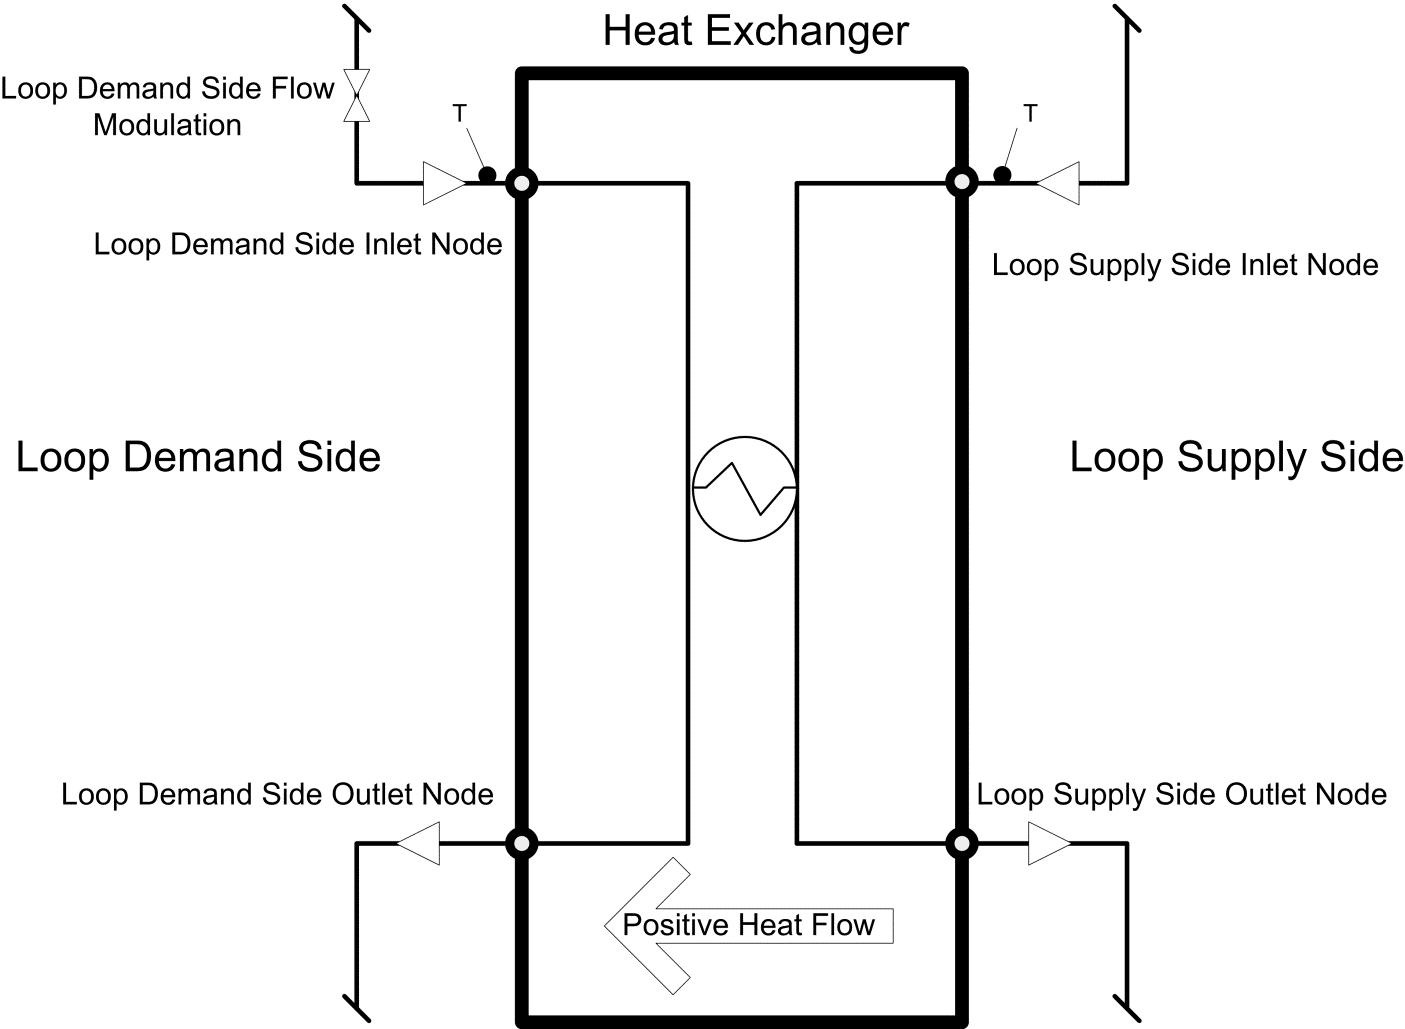
\includegraphics[width=0.9\textwidth, height=0.9\textheight, keepaspectratio=true]{media/image207.png}
\caption{Plant Fluid-to-Fluid Heat Exchanger \protect \label{fig:plant-fluid-to-fluid-heat-exchanger}}
\end{figure}

\textbf{Various options are available for the heat exchanger model.}
\begin{itemize}
\item
    The heat transfer between the two sides can be modeled using one of seven different models for different types of heat exchangers.
\item
    There are also eleven options for different ways to control the heat exchanger.
    \begin{itemize}
        \item
            One general type of control is \textbf{OnOff} where the flow through the heat exchanger is either fully on or fully off.
        \item
            Another type of control is \textbf{Modulated} where the flow through the Loop Demand Side is controlled to try and meet a target setpoint or load on the Loop Supply Side.
    \end{itemize}
\end{itemize}

As of Version 8.0, \textbf{this object replaces three separate objects that were available prior to version 8.0 of EnergyPlus}.
\begin{itemize}
\item
    The former \textbf{HeatExchanger:Hydronic} object corresponds to a situation where the Loop Demand Side is the demand side of condenser loop,
    the Loop Supply Side is a the supply side of a chilled water loop, the control type is ``CoolingSetpointOnOffWithComponentOverride'',
    and the remote override component is a chiller.
\item
    The former \textbf{HeatExchanger:WatersideEconomizer} object corresponds to a situation where the Loop Demand Side is the demand side of condenser loop,
    the Loop Supply Side is a the supply side of a chilled water loop, and the control type is ``CoolingDifferentialOnOff.''
\item
    The former \textbf{HeatExchanger:Plate} object corresponds to a situation where the Loop Demand Side is the demand side of a condenser loop,
    the Loop Supply Side is the supply side of a second condenser loop, and the control type is ``UncontrolledOn.''
\end{itemize}

\subsubsection{Inputs}\label{inputs-15-002}

\paragraph{Field: Name}\label{field-name-13-001}

This alpha field provides the unique identifying name for this heat exchanger.

\paragraph{Field: Availability Schedule Name}\label{field-availability-schedule-name-001}

This field specifies the name of an availability schedule that can be used for supervisory control of the device.~ If blank, the default is that heat exchanger is always available.~ If a scheduled is named here, then the heat exchanger is available for use whenever the schedule value is greater than zero.~ The heat exchanger is not available whenever the schedule value is zero or less.

\paragraph{Field: Loop Demand Side Inlet Node Name}\label{field-loop-demand-side-inlet-node-name}

This field specifies the name of a plant system node that connects an inlet of the heat exchanger to the demand side of a loop.~ This node must be on a branch located on the demand side of a plant or condenser loop.

\paragraph{Field: Loop Demand Side Outlet Node Name}\label{field-loop-demand-side-outlet-node-name}

This field specifies the name of a plant system node that connects an outlet of the heat exchanger to the demand side of a loop.~ This node must be on a branch located on the demand side of a plant or condenser loop.

\paragraph{Field: Loop Demand Side Design Flow Rate}\label{field-loop-demand-side-design-flow-rate}

This field specifies the design flow rate, in m\(^{3}\)/s, of the hydronic fluid passing through the heat exchanger on the Loop Demand Side. This field is autosizable. When autosized, this design flow rate is set to equal the design flow rate for the Loop Supply Side.

\paragraph{Field: Loop Supply Side Inlet Node Name}\label{field-loop-supply-side-inlet-node-name}

This field specifies the name of a plant system node that connects an inlet of the heat exchanger to the supply side of a loop.~ This node must be on a branch located on the supply side of a plant or condenser loop.

\paragraph{Field: Loop Supply Side Outlet Node Name}\label{field-loop-supply-side-outlet-node-name}

This field specifies the name of a plant system node that connects an outlet of the heat exchanger to the supply side of a loop.~ This node must be on a branch located on the supply side of a plant or condenser loop.

\paragraph{Field: Loop Supply Side Design Flow Rate}\label{field-loop-supply-side-design-flow-rate}

This field specifies the design flow rate, in m\(^{3}\)/s, of the fluid passing through the heat exchanger on the Loop Supply Side. This field is autosizable. When autosized, this design flow rate is set equal to the overall design flow rate of the loop that is connected.~ If a sizing factor is entered in the field below, then it is multiplied to modify the design flow rate.

\paragraph{Field: Heat Exchange Model Type}\label{field-heat-exchange-model-type}

This alpha field identifies the nature of heat exchanger.~ Heat exchanger model type is specified by one of the following four key word choices:

\begin{description}
\item [CrossFlowBothUnMixed] Specifies a single-pass, cross-flow heat exchanger. The effectiveness will be calculated using a cross-flow heat exchanger correlation for both streams unmixed.
\item [CrossFlowBothMixed]  Specifies a single-pass, cross-flow heat exchanger. The effectiveness will be calculated using a cross-flow heat exchanger correlation for both streams mixed.
\item [CrossFlowSupplyMixedDemandUnMixed] Specifies a single-pass, cross-flow heat exchanger. The effectiveness will be calculated using a cross-flow heat exchanger correlation for flow mixed on the Loop Supply side and flow unmixed on the Loop Demand Side.
\item [CrossFlowSupplyUnMixedDemandMixed] Specifies a single-pass, cross-flow heat exchanger. The effectiveness will be calculated using a cross-flow heat exchanger correlation for flow unmixed on the Loop Supply side and flow mixed on the Loop Demand Side.
\item [CounterFlow] Specifies a counter-flow shell and tube heat exchanger (one fluid has the opposite direction to the other fluid). The effectiveness will be calculated using a counter-flow shell and tube heat exchanger correlation.
\item [ParallelFlow] Specifies a parallel-flow shell and tube heat exchanger (both fluids have the same direction). The effectiveness will be calculated using a parallel-flow shell and tube heat exchanger correlation.
\item [Ideal] Specifies an ideal heat exchanger. The effectiveness will be set to `1.0' and the specified UA will be ignored. The heat transfer rate will be calculated as the maximum possible heat transfer rate.
\end{description}

For effectiveness of each heat exchanger model type in detail, See "Heat Exchangers: Plant Loop Fluid-to-Fluid Heat Exchanger" Section in Engineering Reference.

\paragraph{Field: Heat Exchanger U-Factor Times Area Value}\label{field-heat-exchanger-u-factor-times-area-value}

This numerical field is used to specify the overall U-Factor Times Area (UA) \{W/K\} for use in the calculation of the heat exchanger effectiveness using the appropriate D-NTU correlation.~ If \textbf{Ideal} is specified as the heat exchanger type, the effectiveness will be set to 1.0. When set to autosize Heat Exchanger U-Factor Times Area Value is calculated based on an effectiveness of 1.0 where capacity is such that the temperatures in the \hyperref[sizingplant]{Sizing:Plant} objects for the two loops can be maintained.

\paragraph{Field: Control Type}\label{field-control-type}

This field is used to specify how the heat exchanger is to be controlled during operation.~ Different applications for connecting two loops will require different control behavior and different control options are needed depending on the desired behavior.~ There are the following eleven key choice options to choose from:

\begin{itemize}
\item
  \textbf{UncontrolledOn}. This control mode is applicable to situations where the heat exchanger is passively running all the time and always transfers as much heat as possible between the fluid streams.~ However there is one aspect of control in that it will only request flow on the Loop Demand Side when there is non-zero flow into the heat exchanger on the Loop Supply Side.~ This control mode corresponds to that available in the HeatExchanger:Plate object prior to version 8.0.
\item
  \textbf{OperationSchemeModulated}.~ This control mode is applicable to situations where the heat exchanger is controlled by an operation scheme (see objects called PlantEquipmentOperationScheme or \hyperref[condenserequipmentoperationschemes]{CondenserEquipmentOperationSchemes}).~ When using this control mode the heat exchanger must be listed in \hyperref[plantequipmentlist]{PlantEquipmentList} or a \hyperref[condenserequipmentlist]{CondenserEquipmentList} and it serves as a supply component.~ The operation scheme will dispatch a load request to the heat exchanger which it will try meet by conditioning the fluid stream connected as the Loop Supply Side.~ If the heat exchanger could exceed the load request, then the flow through the fluid stream connected as the Loop Demand Side will be modulated to just meet the load request.
\item
  \textbf{OperationSchemeOnOff}. This control mode is applicable to situations where the heat exchanger is controlled by an operation scheme (see objects called PlantEquipmentOperationScheme or \hyperref[condenserequipmentoperationschemes]{CondenserEquipmentOperationSchemes}).~ When using this control mode the heat exchanger must be listed in \hyperref[plantequipmentlist]{PlantEquipmentList} or a \hyperref[condenserequipmentlist]{CondenserEquipmentList} and it serves as a supply component.~ The operation scheme will dispatch a load request to the heat exchanger which it will use as an on/off signal to decide if the heat exchange should run or not.~ If it runs, it will run at full capacity and may exceed the load request.
\item
  \textbf{HeatingSetpointModulated}.~ This control mode is applicable to situations where the Loop Demand Side can provide useful heating to the Loop Supply Side.~ A heating setpoint is obtained from a node named in the following field.~ If the setpoint and inlet temperatures are such that heat exchanger could transfer heat from the Loop Demand Side to the Loop Supply Side to meet the heating setpoint, then the heat exchanger will run.~ The inlet temperatures must differ by more than the value set in the field called Minimum Temperature Difference to Activate Heat Exchanger for the heat exchanger to operate. ~If the heat exchanger could overshoot the setpoint, then the flow through the fluid stream connected as the Loop Demand Side will be modulated to just meet the setpoint.
\item
  \textbf{HeatingSetpointOnOff}. This control mode is applicable to situations where the Loop Demand Side can provide useful heating to the Loop Supply Side.~ A heating setpoint is obtained from a node named in the following field.~ If the setpoints and inlet temperatures are such that heat exchanger could transfer heat from the Loop Demand Side to the Loop Supply Side to meet the heating setpoint, then the heat exchanger will run. The inlet temperatures must differ by more than the value set in the field called Minimum Temperature Difference to Activate Heat Exchanger for the heat exchanger to operate. ~If it runs, it will run at full capacity and may overshoot the setpoint.
\item
  \textbf{CoolingSetpointModulated}.~ This control mode is applicable to situations where the Loop Demand Side can provide useful cooling to the Loop Supply Side.~ A cooling setpoint is obtained from a node named in the following field.~ If the setpoints and inlet temperatures are such that heat exchanger could transfer heat from the Loop Supply Side to the Loop Demand Side to meet the cooling setpoint, then the heat exchanger will run. The inlet temperatures must differ by more than the value set in the field called Minimum Temperature Difference to Activate Heat Exchanger for the heat exchanger to operate. If the heat exchanger could undershoot the setpoint, then the flow through the fluid stream connected as the Loop Demand Side will be modulated to just meet the setpoint.
\item
  \textbf{CoolingSetpointOnOff}. This control mode is applicable to situations where the Loop Demand Side can provide useful cooling to the Loop Supply Side.~ A cooling setpoint is obtained from a node named in the following field.~ If the setpoints and inlet temperatures are such that heat exchanger could transfer heat from the Loop Supply Side to the Loop Demand Side to meet the cooling setpoint, then the heat exchanger will run. The inlet temperatures must differ by more than the value set in the field called Minimum Temperature Difference to Activate Heat Exchanger for the heat exchanger to operate. If it runs, it will run at full capacity and may undershoot the setpoint.~ This control mode corresponds to that available in the HeatExchanger:WatersideEconomizer object prior to version 8.0.
\item
  \textbf{DualDeadbandSetpointModulated}. This control mode is applicable to situations where the Loop Demand Side can provide either useful cooling or heating to the Loop Supply Side.~ A dual deadband setpoint is obtained from a node named in the following field.~ If the setpoints and inlet temperatures are such that heat exchanger could transfer heat from the Loop Demand Side to the Loop Supply Side to meet the lower setpoint, then the heat exchanger will run. If the setpoints and inlet temperatures are such that heat exchanger could transfer heat from the Loop Supply Side to the Loop Demand Side to meet the high setpoint, then the heat exchanger will run. The inlet temperatures must differ by more than the value set in the field called Minimum Temperature Difference to Activate Heat Exchanger for the heat exchanger to operate.~ If the heat exchanger could overshoot the lower setpoint, or undershoot the higher setpoint, then the flow through the fluid stream connected as the Loop Demand Side will be modulated to just meet the deadband setpoint.
\item
  \textbf{DualDeadbandSetpointOnOff}. This control mode is applicable to situations where the Loop Demand Side can provide either useful cooling or heating to the Loop Supply Side.~ A dual deadband setpoint is obtained from a node named in the following field.~ If the setpoints and inlet temperatures are such that heat exchanger could transfer heat from the Loop Demand Side to the Loop Supply Side to meet the lower setpoint, then the heat exchanger will run. If the setpoints and inlet temperatures are such that heat exchanger could transfer heat from the Loop Supply Side to the Loop Demand Side to meet the high setpoint, then the heat exchanger will run. The inlet temperatures must differ by more than the value set in the field called Minimum Temperature Difference to Activate Heat Exchanger for the heat exchanger to operate. If the heat exchanger runs, it will run at full capacity and may overshoot the lower setpoint or undershoot the higher setpoint.
\item
  \textbf{CoolingDifferentialOnOff}.~ This control mode is applicable to situations where the Loop Demand Side can provide useful cooling to the Loop Supply Side.~ This mode is similar to CoolingSetpointOnOff except that it ignores any cooling setpoint and its control is based only on the temperature difference between Loop Demand Side and the Loop Supply Side.~ The inlet temperatures must differ by more than the value set in the field called Minimum Temperature Difference to Activate Heat Exchanger for the heat exchanger to operate.~ ~This control mode corresponds to that available in the HeatExchanger:WatersideEconomizer object prior to version 8.0.
\item
  \textbf{CoolingSetpointOnOffWithComponentOverride}.  This control mode is applicable to situations where the heat exchanger operation is integrated with the operation of a specific chiller.  Typically the heat exchanger and chiller are in parallel on separate branches.  When conditions are favorable for the heat exchanger to provide cooling to the Loop Supply Side, the heat exchanger is run and the integrated chiller is turned off.  When conditions are not favorable, the heat exchanger is completely off and the chiller is allowed to run as usual.  A cooling setpoint is obtained from a node named in the following field.  If it runs it will run at full capacity and may undershoot the setpoint.  The chiller that is integrated with the heat exchanger is identified by entering the names of the chiller's inlet nodes in the input fields below.~ The control decision can be based on one of three different temperature signals selected in the field below called Component Override Cooling Control Temperature Mode.~ The setpoint and control signal temperatures must differ by more than the value set in the field called Minimum Temperature Difference to Activate Heat Exchanger for the heat exchanger to operate. This control mode corresponds to that available in the HeatExchanger:Hydronic object prior to version 8.0.
\end{itemize}

\paragraph{Field: Heat Exchanger Setpoint Node Name}\label{field-heat-exchanger-setpoint-node-name}

This field specifies the name of a plant system node located on loop attached to the Loop Supply Side.~ This field is used and required when the previous field is set to one of the ``Setpoint'' control types.~ The node must have a temperature setpoint placed on it by a setpoint manager (or EMS actuator).

If the previous field is set to DualDeadbandSetpointModulated or DeadbandSetpointOnOff then there must be a setpoint manager that places both a high and low setpoint on the node named in this field. (see \hyperref[setpointmanagerscheduleddualsetpoint]{SetpointManager:Scheduled:DualSetpoint}).

\paragraph{Field: Minimum Temperature Difference to Activate Heat Exchanger}\label{field-minimum-temperature-difference-to-activate-heat-exchanger}

This field specifies the value of a temperature tolerance used in control decisions, in deg. Celsius.~ Whenever the control logic needs to compare two temperatures, the value entered in this field is used as a threshold for comparisons.

\paragraph{Field: Heat Transfer Metering End Use Type}\label{field-heat-transfer-metering-end-use-type}

This field specifies how the metering for heat transfer will be accounted with respect to end uses.~ Although the heat exchanger consumes no energy that needs to be metered, there are also meters for heat transfers that apply to the model. The nature of the end use may vary depending on the application that the heat exchanger is being used for.~ The available choices are FreeCooling, HeatRecovery, HeatRejection, HeatRecoveryForCooling, HeatRecoveryForHeating, and LoopToLoop.

\paragraph{Field: Component Override Loop Supply Side Inlet Node Name}\label{field-component-override-loop-supply-side-inlet-node-name}

This field specifies the name of an inlet node for the remote component that will be integrated with this heat exchanger.~ This inlet should be on the supply side of a loop -- typically chilled water inlet or return for a chiller.~ This field and the next two are only used for the control type called CoolingSetpointOnOffWithComponentOverride.

\paragraph{Field: Component Override Loop Demand Side Inlet Node Name}\label{field-component-override-loop-demand-side-inlet-node-name}

This field specifies the name of an inlet node for the remote component that will be integrated with this heat exchanger.~ This inlet should be on the demand side of a loop -- typically condenser water inlet or return for a water-cooled chiller.~ This field is only used for the control type called CoolingSetpointOnOffWithComponentOverride.

\paragraph{Field: Component Override Cooling Control Temperature Mode}\label{field-component-override-cooling-control-temperature-mode}

This field specifies which type of temperature is used to control a heat exchanger that uses the control type called CoolingSetpointOnOffWithComponentOverride.~ There are three options: Loop, WetBulbTemperature, and DryBulbTemperature.~ The option called ``Loop'' directs the program to use the inlet fluid temperature at the Loop Demand Side connection of~ heat exchanger for the temperature used as a signal to be compared with the setpoint. The option call ``WetBulbTemperature'' uses the outdoor air wetbulb temperature as the signal.~ The option called ``DryBulbTemperature'' uses the outdoor air drybulb temperature as the signal.

\paragraph{Field: Sizing Factor}\label{field-sizing-factor-4}

This optional field can be used to modify the results of autosize calculations.~ This sizing factor is used for this heat exchanger and modifies sizing results by multiplying them by the factor entered here.~ This factor is applied to the Loop Supply Side Design Flow rate and in turn affects the heat exchanger UA and the loop demand side flow rate which are derived from that flow rate.~ This allows fine control over the size of the heat exchanger when using autosize in those fields.

\paragraph{Field: Operation Minimum Temperature Limit}\label{field-operation-minimum-temperature-limit}

This optional field can be used to provide supervisory control of the heat exchanger. If either of the inlet temperatures are below this limit (°C), the heat exchanger will not operate.

\paragraph{Field: Operation Maximum Temperature Limit}\label{field-operation-maximum-temperature-limit}

This optional field can be used to provide supervisory control of the heat exchanger. If either of the inlet temperatures are above this limit~ (°C), the heat exchanger will not operate.

Some example IDF input objects follow.

\begin{lstlisting}

  HeatExchanger:FluidToFluid,
      CondenserLoop HX,!- Name
      ALWAYS_ON,     !- Availability Schedule Name
      CondenserLoop HX HX Inlet Node, !- Loop Demand Side Inlet Node Name
      CondenserLoop HX HX Outlet Node, !- Loop Demand Side Outlet Node Name
      autosize,                     !- Loop Demand Side Design Flow Rate
      CondenserLoop Pump- HXNode,   !- Loop Supply Side Inlet Node Name
      CondenserLoop HX- ChillerNode,!- Loop Supply Side Outlet Node Name
      autosize,                !- Loop Supply Side Design Flow Rate
      CounterFlow,             !- Heat Exchange Model Type
      autosize,                !- Heat Exchanger U-Factor Times Area Value
      CoolingDifferentialOnOff,    !- Control Type
      ,   !- Heat Exchanger Setpoint Node Name
      2.0,         !- Minimum Temperature Difference to Activate Heat Exchanger
      FreeCooling;             !- Heat Transfer Metering End Use Type


  HeatExchanger:FluidToFluid,
      SOURCE to TRANSFER HX , !- Name
      AlwaysOnSchedule, !- Availability Schedule Name
      SOURCE Demand HX Inlet Node , !- Loop Demand Side Inlet Node Name
      SOURCE Demand HX Outlet Node , !- Loop Demand Side Outlet Node Name
      0.003 , !- Loop Demand Side Design Flow Rate
      TRANSFER HX Supply Inlet Node, !- Loop Supply Side Inlet Node Name
      TRANSFER HX Supply Outlet Node, !- Loop Supply Side Outlet Node Name
      0.003 , !- Loop Supply Side Design Flow Rate
      CrossFlow, !- Heat Exchange Model Type
      15000 , !- Heat Exchanger U-Factor Times Area Value
      DualDeadbandSetpointModulated , !- Control Type
      TRANSFER Supply Outlet Node, !- Heat Exchanger Setpoint Node Name
      0.2 , !- Minimum Temperature Difference to Activate Heat Exchanger
      LoopToLoop; !- Heat Transfer Metering End Use Type
\end{lstlisting}

\subsubsection{Outputs}\label{outputs-15}

\paragraph{Fluid Heat Exchanger Heat Transfer Rate {[}W{]}}\label{fluid-heat-exchanger-heat-transfer-rate-w}

\paragraph{Fluid Heat Exchanger Heat Transfer Energy {[}J{]}}\label{fluid-heat-exchanger-heat-transfer-energy-j}

These outputs are the rate and energy transferred from the Loop Supply Side to the Loop Demand Side.~ The sign convention is taken from cooling or heat rejection applications such that positive values indicate cooling of the Loop Supply Side.

\paragraph{Fluid Heat Exchanger Loop Supply Side Mass Flow Rate {[}kg/s{]}}\label{fluid-heat-exchanger-loop-supply-side-mass-flow-rate-kgs}

This is the system mass flow of fluid through the heat exchanger side connected as the Loop Supply Side, in kg/s.

\paragraph{Fluid Heat Exchanger Loop Supply Side Inlet Temperature {[}C{]}}\label{fluid-heat-exchanger-loop-supply-side-inlet-temperature-c}

This is the temperature, in degrees Celsius, of the fluid entering the heat exchanger on the side connected as the Loop Supply Side.

\paragraph{Fluid Heat Exchanger Loop Supply Side Outlet Temperature {[}C{]}}\label{fluid-heat-exchanger-loop-supply-side-outlet-temperature-c}

This is the temperature, in degrees Celsius, of the fluid leaving the heat exchanger on the side connected as the Loop Supply Side.

\paragraph{Fluid Heat Exchanger Loop Demand Side Mass Flow Rate {[}kg/s{]}}\label{fluid-heat-exchanger-loop-demand-side-mass-flow-rate-kgs}

This is the system mass flow of fluid through the heat exchanger side connected as the Loop Demand Side, in kg/s.

\paragraph{Fluid Heat Exchanger Loop Demand Side Inlet Temperature {[}C{]}}\label{fluid-heat-exchanger-loop-demand-side-inlet-temperature-c}

This is the temperature, in degrees Celsius, of the fluid entering the heat exchanger on the side connected as the Loop Demand Side.

\paragraph{Fluid Heat Exchanger Loop Demand Side Outlet Temperature {[}C{]}}\label{fluid-heat-exchanger-loop-demand-side-outlet-temperature-c}

This is the temperature, in degrees Celsius, of the fluid leaving the heat exchanger on the side connected as the Loop Demand Side.

\paragraph{Fluid Heat Exchanger Operation Status {[}0 = off, 1 = on{]}}\label{fluid-heat-exchanger-operation-status-0-off-1-on}

This output is a numeric flag that indicates whether or not the heat exchanger was operating or not.~ If the value is 0, then the heat exchanger was not operating.~ If the value is 1, then the heat was operating.

\paragraph{Fluid Heat Exchanger Effectiveness {[]}}\label{fluid-heat-exchanger-effectiveness}

This output is the calculated heat exchanger effectiveness (non-dimensional).~ It is an intermediate value in the NTU model calculations for heat flow rate.~ Values range between 0 and 1.0.~ A value of 1.0 indicates ideal heat transfer.
